
\documentclass[a4paper,english]{report}
\usepackage{subfiles}
\usepackage[utf8]{inputenc}
\usepackage{babel,duomasterforside}
\usepackage[backend=biber]{biblatex}
\bibliography{library.bib}
\usepackage{csquotes}
\usepackage{pdfpages}
\usepackage{graphicx}
\usepackage{mathtools}
\usepackage{amsmath}
\usepackage{amssymb}
\usepackage{subcaption}
\usepackage[nottoc,numbib]{tocbibind}
\usepackage{titlesec}
\usepackage{subfiles}
\usepackage{listings}
\usepackage[export]{adjustbox}[2011/08/13]
\titleformat{\chapter}{\normalfont\huge\bf}{\thechapter.}{20pt}{\huge\bf}



\title{Master Thesis}
\subtitle{Transfer learning and modularity in a Super Neural Network}
\author{Martin J. Hovin}

\begin{document}
\duoforside[dept={Institute for informatics},
program={Nanoelectronics and Robotics: Robotics and Intelligent Systems},
long]


\newenvironment{acknowledgements}%
    {\cleardoublepage\thispagestyle{empty}\null\vfill\begin{center}%
    \bfseries Acknowledgements\end{center}}%
    {\vfill\null}
        \begin{acknowledgements}
            Who is your advisor? 
            Did anyone help you? 
            Who funded this work? 
            What's the name of your favorite pet?
        \end{acknowledgements}


\begin{abstract}
    What is all this about? 
    Why should I read this thesis? 
    Is it any good? 
    What's new? 
\end{abstract}




\tableofcontents
\listoffigures
\listoftables

\chapter{Introduction}

\section{Some background etc}
\section{Some motivation}

\chapter{Theoretical Background}
Since Turing wrote about the imitation game\cite{imitationgame} and Rosenblatt about the perceptron\cite{perceptron}, learning machines have stayed in the minds of computer scientists and science fiction writers. 
Improvements in computation and algorithms have since then taken machine learning(ML) past human level performance in multiple areas such as image recognition\cite{youtubecats}\cite{deepface}, board games like chess\cite{alphazero} or go\cite{alphago}, TV game-shows like Jeopardy\cite{jeopardy} or e-sports such as DOTA2\cite{dota2}.

\section{Machine Learning}\label{background:ML}
 
In machine learning, the fields of statistics, mathematics and data analysis are combined and applied to automatic modeling of data. Its three main sub-fields, supervised, unsupervised and reinforcement learning covers a vast number of structures and techniques, but in this thesis we will focus on the flag-ship of machine learning, the artificial neural network, and set it in a supervised learning scenario where it is applied to a classification problem.

\begin{figure}[h] 
\centering
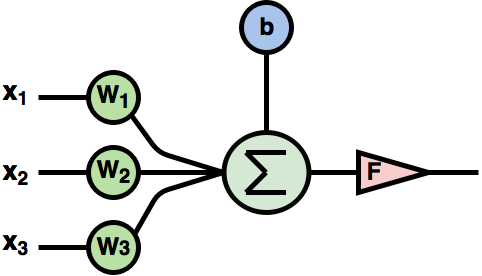
\includegraphics[width=0.7\linewidth]{Chapters/Background/figures/artificial_neuron.png}
\caption{Visualization of a artificial neuron. Each input \(x_{i}\) is multiplied with a corresponding trainable weight \(W_{i}\) before the products are all summed together with a bias \(b\). The resulting value is then passed through a activation function \(F\)}
\label{fig:artificialneuron}
\end{figure}

Supervised learning is a way to teach some machine learning system patterns in annotated data. In a data set \(\left [X, Y \right] \), each data-point \(x_{i}\) corresponds to a label or ground truth \(y_{i}\). In the context of a Artificial Neural Network, each \(x_{i}\) is fed through the network and fitted against the target \(y_{i}\) using some optimization algorithm. 

Inspired by the structure of the brain, the \textit{Artificial Neural Network} or \textit{Neural Network} (NN) consists of layers of artificial neurons like the one visualized in figure \ref{fig:artificialneuron}. Each neuron has a number \(n\) of inputs \(x_{i}\) where each input is scaled by a tunable parameter or \textit{weight} \(w_{i}\) and summed together including a bias \(b\) before it is passed through a activation function \(F\).

\begin{equation}
    F(\sum_{i=1}^{n}W_{i}x_{i} + b) = output
\end{equation}

Two of the most commonly used activation functions are the rectified linear unit function (ReLU) and the softmax function, which is the generalization of binary logistic regression to multiple classes. ReLU simply evaluates to the maximum of neuron output and 0, which sets zero if the output is negative and keeps positive outputs. Softmax on the other hand approximates a probability by scaling the output of a set of neurons to have a sum between 0 and 1 and are used in classification. These two activation functions will play a role in the later experiments (see \ref{exp1:implementation} and \ref{exp2:implementation}) in this thesis, where softmax will be used as the final activation layer to be the basis of classification. ReLU is used as activation function throughout the rest of the neural networks. 

These types of systems \textit{learn} to approximate a function based on the data provided to the network. Each data point x consist of multiple features (\(x_{i}\)'s), which is fed through one or more layers of neurons that outputs an prediction \(\hat{y}_{i}\). This prediction is then compared to the ground truth with a loss function\footnote{Also called cost function, error function or objective function} which calculates the difference between expected output \(y_{i}\) and observed output \(\hat{y}_{i}\). Here also there is a multitude of functions which will not be discussed. For the purpose of classification in this thesis, the loss function we will use is a cross-entropy function which is well suited for classification with the softmax activation output\cite{softmaxcrossentropy}.

The goal of the training is to minimize the loss function for a given data set. To accomplish this, the loss is backpropagated through the neural network and an optimization algorithm is used to calculate the gradient of the weights with regards to the layer output and then to adjust the weights. The optimizers used in the experiments \ref{exp1} and \ref{exp2} are stochastic gradient descent(SGD)\cite{sgd} and Adaptive Moment Estimation (Adam)\cite{adam}. 

Neural Networks function approximation properties can be used in regression in data analysis or reward signal estimation in reinforcement learning among other things, but are as mentioned applied to classification in this thesis. 
The final softmax layer outputs an estimated probability for each label given some input where the label given highest probability is selected as the models prediction. As long as the input features to the network is correlated to the label in some way and there is enough training data, the neural network will adapt to the patterns in input features and learn one or more classification rules. In the case of a image classification problem, the network is provided with the raw pixel values in the image. A normal, fully connected neural network\footnote{Also called affine or dense networks or layers} is badly suited for this type of classification since attributes in images often change location or scale in the images\ref{exp1:implementation}. E.g: a picture of a dog is still a image of a dog if you rotate the image upside down, zoom in on the dog or frame the image differently. To account for all these cases, the data set used would have to contain enough examples of all these variations.
\begin{figure}[h] 
    \centering
    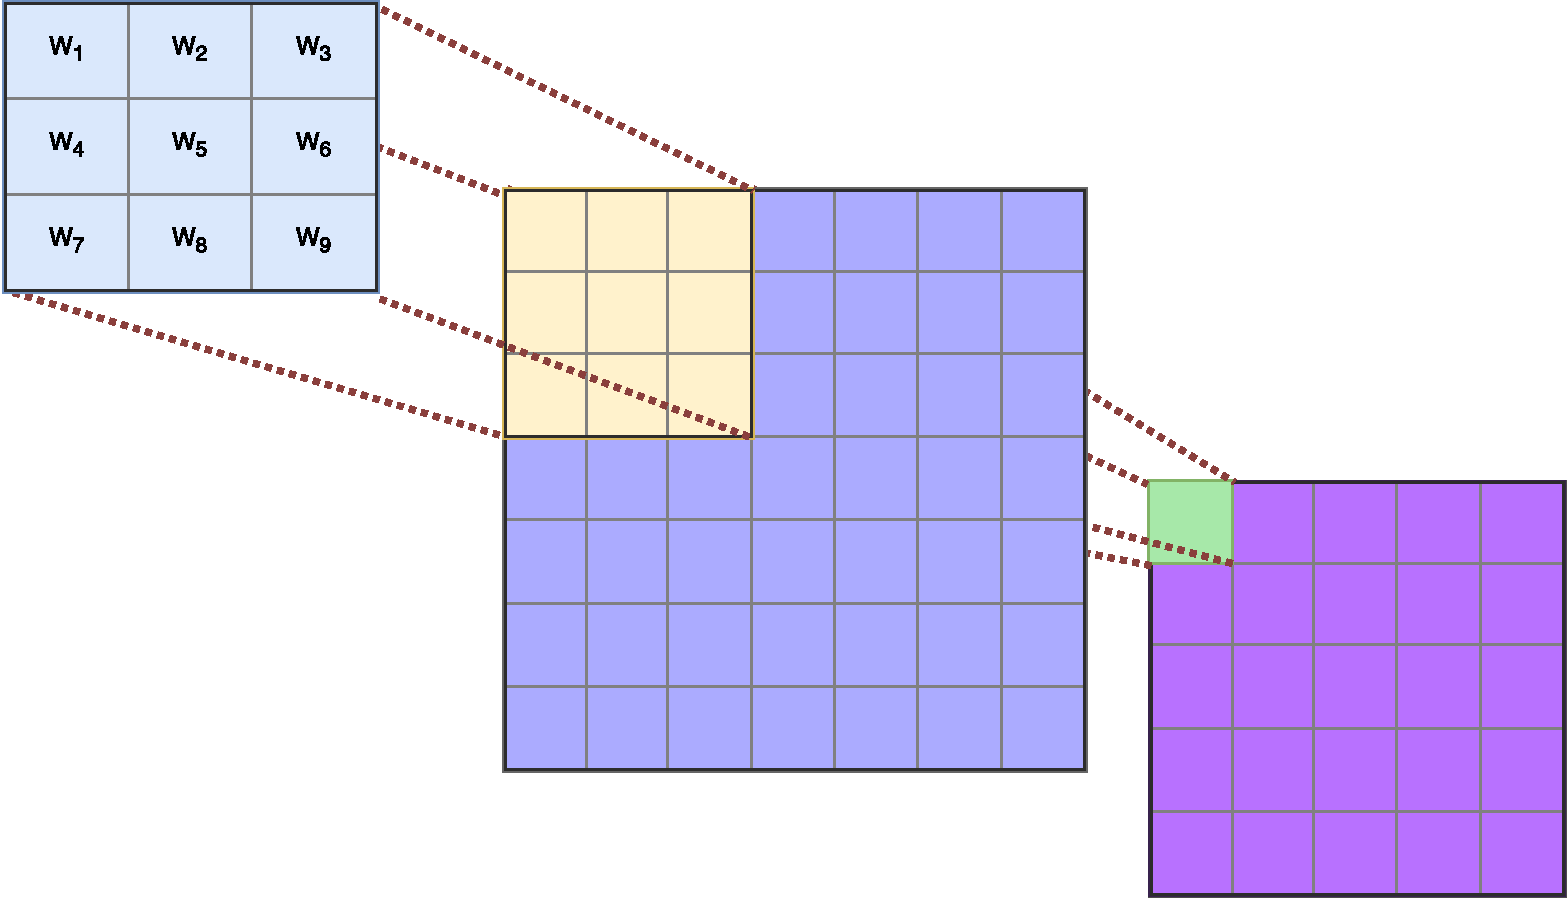
\includegraphics[width=\linewidth]{Chapters/Background/figures/convolution.pdf}
    \caption{Illustration of convolutional operation. The teal matrix contain convolutional parameters. These are element-wise multiplied by the overlapping (yellow) pixels in the image (blue) and added together. The resulting value is placed in the corresponding location in the output feature map (purple). The convolutional operation is completed by sliding or \textit{striding} the yellow window across the original image.}
    \label{fig:conv}
\end{figure}
To remedy this problem, image classification usually contain convolutional layers which are invariant to scale, rotation or translation. In a convolutional layer, a \textit{kernel} of trainable weights are convolved with the input image. This results in what is called a feature map, where the image size is reduced by some number of pixels\footnote{In some cases we would want to keep the image dimensions, in which case the input image can be padded to keep its original form.} depending on the size of the kernel, but the depth of the image (number of channels) is increased, the intent being each feature map contains more abstract information than the previous one. 

In a convolutional operation, a kernel is slid across an image, and for every overlap between the kernel and a image section, the kernel weights are multiplied with its corresponding pixel and summed (see \ref{fig:conv}). As with fully connected layers, the operations performed in each step is multiplication and summation, but here, each pixel in the output feature map contains some spatial information.
This spatial area covered by each feature can be controlled by the kernel size and how much the kernel is moved (called stride) between each kernel multiplication.
Networks consisting of multiple layers of convolution is called convolutional Neural Networks (CNNs)\footnote{These is the types of modules used in implementing the quinary MNIST classification in \ref{exp1}, and the whole of \ref{exp2}}.

\begin{figure}[h] 
    \centering
    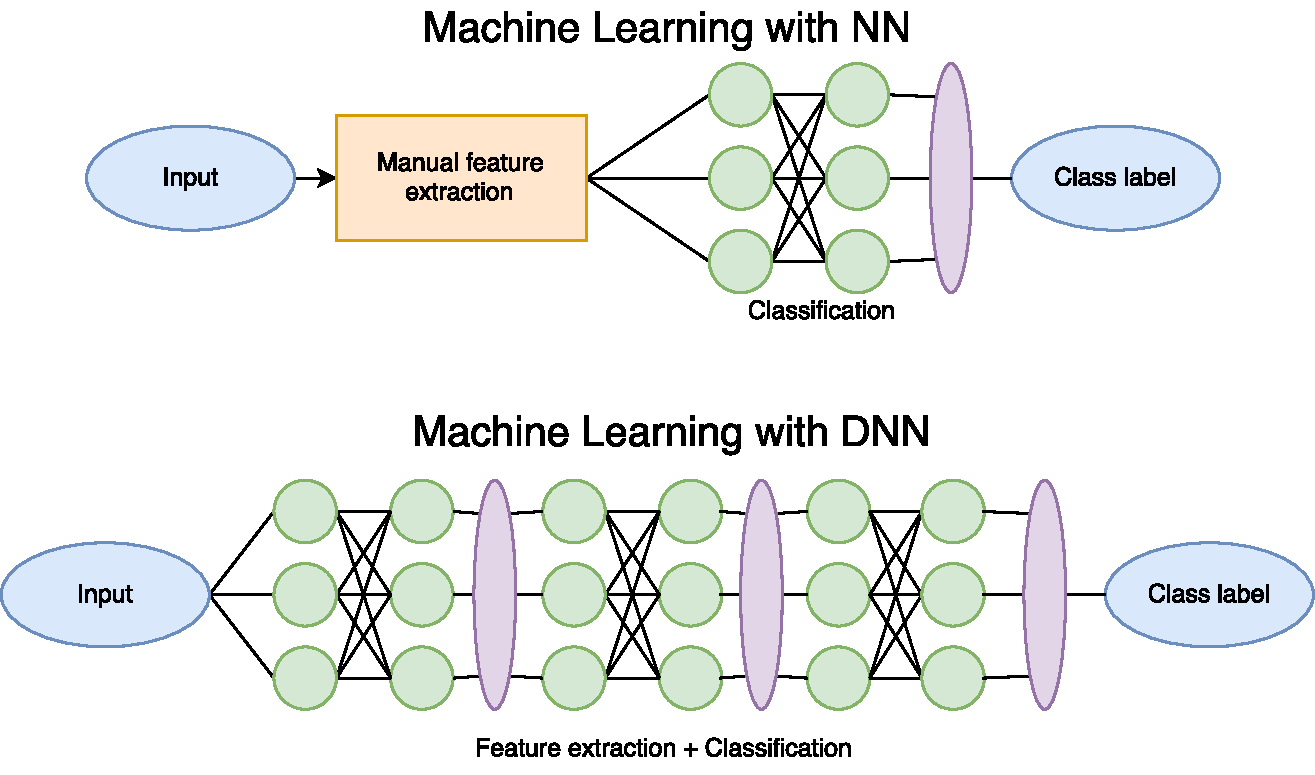
\includegraphics[width=0.8\linewidth]{Chapters/Background/figures/NNvsDNN.pdf}
    \caption{Figure visualizes the difference between traditional Neural Networks and Deep Neural Networks. Artificial neurons (\textit{green}) are fully connected in both cases, and an activation layer (\textit{purple}) is set after every two layers. Where classical NN depends on being provided with high order features, the DNN performs its own feature extraction in its first layers.}
    \label{fig:NNvsDNN}
\end{figure}

\section{Deep Learning}
Usually when talking about CNNs, the line is crossed into what is described as Deep Learning. In each layer of convolution, the spatial size is reduced while the number of channels is increased. This means the information worked on for each step gradually shifts from a spatially encoded image of sorts to a encoding in feature space. This makes a full CNN capable of turning raw image input into a higher order feature representation which can be used in classification. This is why deep Convolutional Neural Networks can be said to be Neural Networks that performs its own feature extraction from raw data.

\begin{figure}
    \begin{subfigure}[h]{0.49\linewidth}
        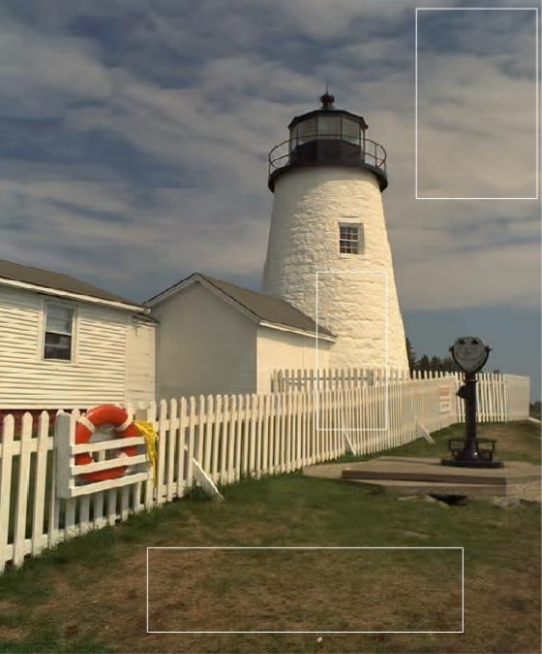
\includegraphics[width=\linewidth]{Chapters/Background/figures/original.png}
        \caption{Original image}
    \end{subfigure}
    \hfill
    \begin{subfigure}[h]{0.49\linewidth}
        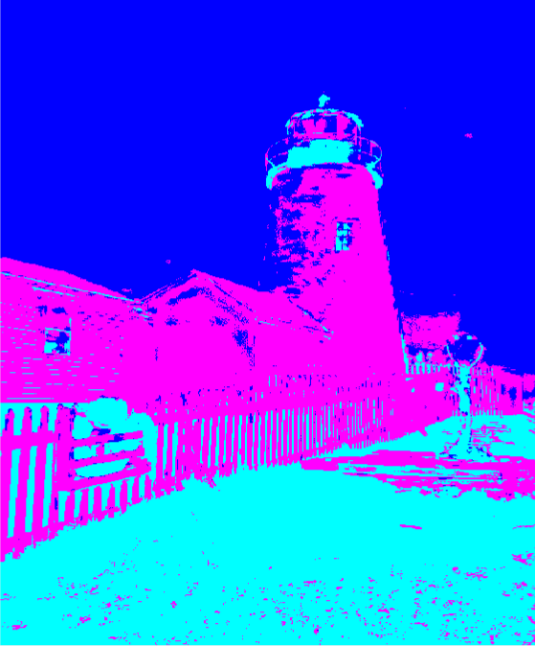
\includegraphics[width=\linewidth]{Chapters/Background/figures/segmentation.png}
        \caption{Segmented image}
    \end{subfigure}
    \caption{Example of image segmentation. Original image have been segmented into three classes: \textit{sky}, \textit{ground} and \textit{building}. The three boxes in the original image is pixels used as training data for each class.}
    \label{fig:semanticsegmentation}
\end{figure}

How \textit{deep} a DNN is made depends on the task at hand. Take for example a complex task such as \textit{semantic segmentation}. Semantic segmentation is a variation of image classification where each pixel in a input image is assigned a class label, and the whole of the image can segmented into its parts (see figure \ref{fig:semanticsegmentation}). In such a CNN, the spacial information in the original image can not be removed completely since we want to create a new image with the original dimensionality and spacial locations of objects. Such a NN would need to have enough \textit{capacity} to retain all needed knowledge to complete the task. The capacity of a NN is how much information is able to be stored in its weights, and is a measure highly correlated to the NNs number of parameters. Managing capacity needs of a NN is part of the motivation behind encouraging module reuse in experiments 1 and 2 (see \ref{exp1} and \ref{exp2}).

Intuitively, the difference between NNs and Deep neural networks (DNN) is just the number of layers in the model, but functionally we can view the DNN as a collection of \textit{shallow} learning models, defined through the use of activation functions as seen in \ref{fig:NNvsDNN}. Complex Deep Learning models have been effective at such tasks as image classification\cite{imageclassification}, natural language processing\cite{deepnlp} and Reinforcement Learning\cite{deepreinforcementlearning}. The architecture and use of each of these types of DNNs are dependent on the input type and problems they are applied to as well as resource limitations.

\textbf{Edit note: Need more about DL?}

The large number of trainable parameters in deep learning increase the data resources needed. If the amount of available labeled training data is restricted, one solution is to train on a similar task for which there is a good amount of data and apply what is learned to the original task. It is shown that this reuse of knowledge as a basis for further learning yields better results that was possible with the original data set\cite{pathnet, progressiveneuralnetworks, tradaboost}. 

\subsection{Transfer Learning}
The approach of Transfer Learning (TL) is to use generalized knowledge in one domain as a basis for future learning in another. With the goal of achieving more effective learning in the target domain or even reaching a lower convergence point for the loss, TL shares some common ground with the field of multi-task learning, where the same model is applied to multiple tasks. 

We can define transfer learning as trying to learn a target conditional probability distribution \(P(Y_{t}|X_{t})\) within a domain \(\mathcal{D}_{t}\), based on information gained from learning a source task \(\mathcal{T}_{s}\) in the source domain \(\mathcal{D}_{s}\) where \(\mathcal{D}_{s} \neq \mathcal{D}_{t}\) and \(\mathcal{T}_{s} \neq \mathcal{T}_{t}\). A domain \(\mathcal{D}\) would then, in a typical classification example, be given as \(\mathcal{D} = \{X, P(X)\}\) where \(X = x_{1},x_{2}, \dotsc ,x_{n}\) are sampled from the feature space \(\mathcal{X}\) and \(P(X)\) is a probability distribution over that space. The task \(\mathcal{T}\) in that domain would then consist of a label space \(\mathcal{Y}\) and the conditional probability distribution \(P(Y|X)\) which usually is approximated during training on a set of \(x_{i}, y_{i}\) pairs where \(x_{i} \in \mathcal{X}\) and \(y_{i} \in \mathcal{Y}\).
\newline\newline

Traditionally, transfer learning has been applied in three ways: 
\begin{enumerate}  
    \item Replacing the last layer in some trained NN. For example using the first layers of a CNN image classifier as feature extraction for some other image classification task 
    \item Fine tuning a trained NN by restarting a back propagation sequence for new data from a domain \(\mathcal{D}_{t}\)
    \item A combination of the preceding techniques where the last layers of a NN is replaced and trained from scratch, and the loss for these layers are back propagated through the rest of the already trained net.
\end{enumerate}


\begin{figure}[h] 
    \centering
    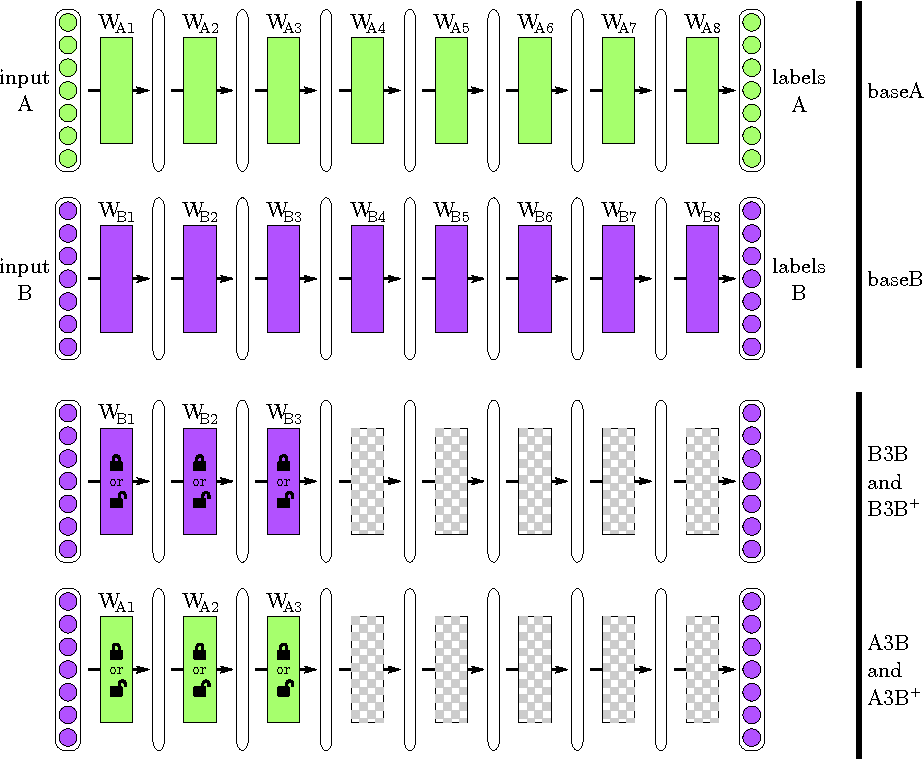
\includegraphics[width=\linewidth]{Chapters/Background/figures/transfer_experiment.png}
    \caption{Illustration provided by Yosinski et al. in their paper\cite{yosinski2014transferable} in figure 1 to visualize their experimental process. The top two models A (green) and B (purple) are trained first on data A and data B. The labeled rectangles represents each layer in the networks, i.e. \(W_{A_{1}}\) is the weights in layer 1 in model A and the ellipsoids between each layer represents activation layers. The color of the stack of circles to the left of each model shows which partition of the data set each model is trained on(again A is green and B is purple). The bottom two rows show the first three layers from A and B being transferred to new randomly initialized models. In the paper they showed they found better accuracy in model A3B than every other model in this figure, even B3B.}
    \label{fig:transferexperiment}
\end{figure}

In a study by Yosinski et al. \cite{yosinski2014transferable}, results showed transferability in the first layers of an image classifier during an experiment proposed to measure generality and specificity in the layers as transfer performance. The study divided the data set\footnote{The study used the ImageNet dataset of 2012 which contained 1,281,167 labeled training images and 50,000 test images, each labeled with one of 1000 classes.} randomly in two subsets (A and B), and trained two identical models on each of the subsets. Replacing the first n layers in two randomly initialized other models with the first \(n\) layers from the trained models (one from A, and one from B), they did an additional training step (fine-tuning by allowing back propagation through the copied layers in some cases) on data from subset B only. This is visualized in figure \ref{fig:transferexperiment} for \(n=3\). The goal was to study the effects transferring layers from one classification case to another had on accuracy. The best results reached were achieved when training a model on subset A, transferring the first three layers to a new randomly initialized model and fine-tuning these transferred layers while training the newly formed on data from subset B. This confirmed their expectation that the earlier layers in a image classifications scenario learns to approximate Gabor-filters which are highly generalized. In section \ref{exp1:results} we see tendencies to this behaviour. 

\subsection{Multi-task Learning}
Multi-task Learning and Transfer Learning both have the same ideology of sharing some parameter state between tasks to positively influence learning. Where Transfer Learning does not concern itself with performance on a seed task, multi-task learning try to optimize parameters for multiple tasks. The most common ways of achieving this is by \textit{soft parameter sharing} and \textit{hard parameter sharing}. While both techniques have some weights unique to each task, \textit{hard parameter sharing} optimize the same parameters for all tasks. This is shown to significantly reduce overfitting\cite{hardparametersharing}. As the weights change values to optimize for a changing target, they never overly adapt to the training set. \textit{Soft parameter sharing} on the other hand have separate parameters for each task, but lateral connections between each tasks layers to minimize the distance between the parameters trained for each task.

\subsection{Curriculum Learning}
Both humans and animals learn better when examples provided is ordered and gradually increasing in difficulty. With this motivation, curriculum learning is introduced as strategy for optimizing the learning process. This technique is shown to increase generalization to data\cite{curriculumlearning} and is the motivation for task ordering in the selection pressure experiments (see \ref{exp2:datasets}).

\section{Catastrophic Forgetting}
A problem that arises in systems where parameters is trained on multiple sequential tasks is what is called \textit{catastrophic forgetting}. Not discussed by Yosinski, but set in a transfer learning scenario, this effect manifests itself as moving parameters away from an area of low error for a previously trained task. This movement could for instance be because the parameters is fine tuned for a new task. While the performance for the second task increase, performance for the first task decrease because the \textit{knowledge is forgotten} when the weights are re-adapted to the new data. This is not a problem in a scenario where the source task is considered a stepping stone to reach good performance for the target task, but might be if all tasks trained on are of the same importance.

\begin{figure}[h]
    \centering
    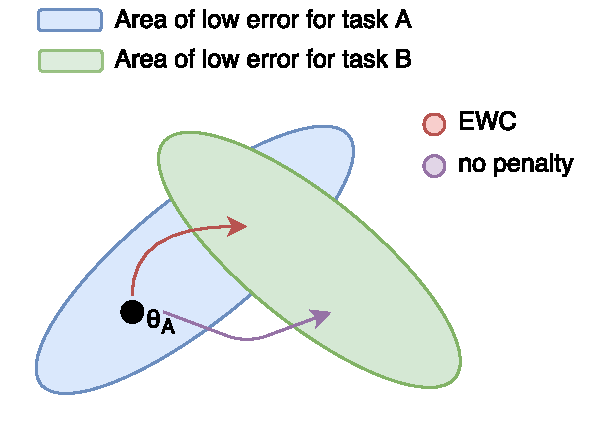
\includegraphics[width=0.7\linewidth]{Chapters/Background/figures/EWC.pdf}
    \caption{Figure from the paper on reducing catastrophic forgetting\cite{ewc}. The figure shows the parameter space \(\mathcal{P}\) and hypothetical areas of low error for two tasks A and B. The arrows indicate the direction EWC \textit{red} and normal training \textit{purple} takes the parameters.}
    \label{fig:ewc}
\end{figure}

\subsection{Elastic Weight Consolidation}
Elastic Weight Consolidation (EWC) is a novel algorithm proposed in January of 2017 by Kirkpatrick et al.\cite{ewc}. During the transfer of weights from task A to task B, over-parameterization makes it likely that a solution to problem B\footnote{A solution may be viewed as a set of parameters \(\bar{\theta}\). Training a NN consists of adjusting these parameters through the process of back propagation with the gradient descent algorithm. For multiple parameters in \(\bar{\theta}_{A}\), many configurations of those values will give the same performance for the NN.} lays close to the solution for task A in the parameter space \(\mathcal{P}\). During optimization of \(\bar{\theta}\) for task B, EWC makes sure the parameters stay within an area of low error for task A as seen in figure \ref{fig:ewc}

Using EWC, Kirkpatrick et al.\cite{ewc} was able to train the same NN on 10 different Atari games without the effects of catastrophic forgetting between training tasks. With a human-normalized score of 1 for each game, giving a total possible score\footnote{where is 0 the same as a random agent, and 10 is at least human-level performance on all games.} of 10, the EWC driven training reached a score of around 6 after 500 million training frames, while the control never reached anything higher than 1.

\subsection{Progressive Neural Networks}
Rusu et al. published a paper in September of 2016\cite{progressiveneuralnetworks} where they addressed the problem of catastrophic forgetting during transfer learning with fine-tuning. Their proposed solution, Progressive Neural Networks (PNN) were shown to be able to learn multiple tasks sequentially without overwriting the previously trained weights. This was done by horizontally scaling the DNN with a new stack of layers for each new task the structure was applied to.
\begin{figure}[h]
    \centering
    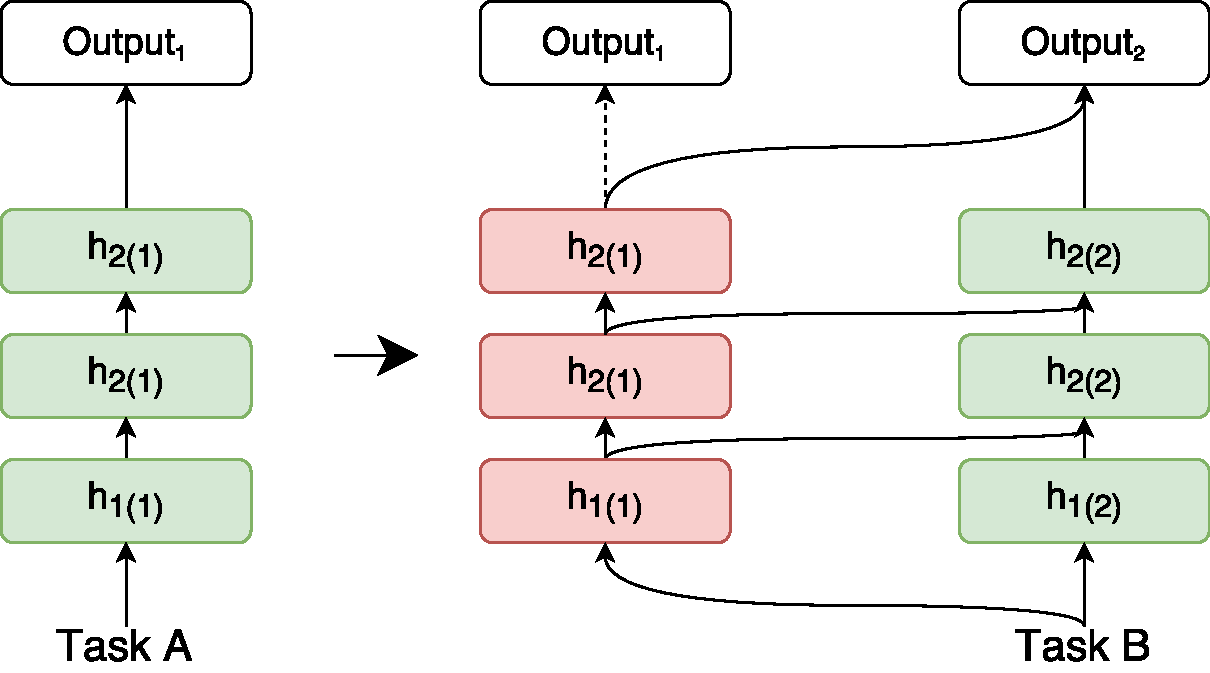
\includegraphics[width=0.8\textwidth]{Chapters/Background/figures/ProgressiveNeuralNet.pdf}
    \caption{Example of a PNN. \textit{Left}: a three-layer NN is trained on task A. \textit{Right}: Adding another stack of three hidden layers that are being trained on task B. The weights in the first stack trained on A is now locked to the back propagation from task B, but its weights may be used is shown by arrows between the layers. Green indicates layer is open to back propagation, red indicates it is locked. Note that injection of a layer from a older task is not possible as lateral connections are only \textit{to} the new layer. The figure is a simplification of multiple figures from the article\cite{progressiveneuralnetworks}}
    \label{fig:pnn}
\end{figure}
After training a DNN on a task A\footnote{In the paper, the PNN is focused as an application for Reinforcement tasks where the PNN were trained to provide probabilities over actions from a set of possible actions, from an input state.}, a new DNN were initialized with lateral connections (see fig. \ref{fig:pnn}) to the NN trained on task A and then trained on task B with back propagation only done through the newly initialized layers. This ensures that the new DNN can optimize freely on task B, but will be able to utilize the weights trained on task A, without catastrophic forgetting occurring in the first DNN. When a sufficient performance on task B is reached, the PNN is able to perform optimally on both tasks, given some selection of the output (i.e: if given data for a task within the domain A, the output from the weights trained on task B is not optimal). Multiple tasks can be trained using this method. For each new task, a new DNN is initialized and the other DNNs in the PNN is connected laterally to each new layer. 

We can compare the way each new task is learned to a transfer learning scenario where backpropagation is locked in the transferred layers (see figure \ref{fig:transferexperiment}). The difference being the layer outputs are calculated in parallel for the two models and multiple of these outputs may be introduced in the new model through what the paper calls \textit{adapters} (not visualized in \ref{fig:transferexperiment}). These \textit{adapters} performs dimensionality reduction as well as tunable scalars so the model can scale lateral connections as needed for the new task.

A problem with this scaling raised and addressed in the paper is that of quadratic growth of parameters for each new training task. Experiments show that there is a reduction in the new capacity actually utilized by the PNN for each new task added. This implies the growth of the PNN for each new task could decrease exponentially\footnote{Here the paper suggests pruning or online compression during learning.} without needing the new task to follow the same downward trend in complexity. 

\section{Genetic Algorithms}
Falling in a sub-category of evolutionary algorithms, genetic algorithms (GA) are biologically inspired algorithms that generate high-quality solutions to optimization and search problems. By mimicking natural operators like \textit{crossover} and \textit{mutation}, GAs views its possible solutions as individual genomes in a population, and applies these natural operators on the population in a simplification of how evolution works. 

An important driving force of GAs is the fitness-function, which maps a genome to a fitness value that can be used to rank solutions (genotypes) by how well they perform. In a natural example of the fitness function, a strong animal of some sort able to acquire nourishment and fend of potential predators is given a higher fitness value than a similar animal not as well suited for its environment. The famous term \textit{survival of the fittest} is valid in both this example and the \textit{in silico} representation of evolution. The strongest animal has a higher probability to survive and reproduce, and GAs are implemented to favour solutions that yield high fitness values.  
When a population is ranked by its fitness, different selection schemes can be applied to simulate the natural selection of the strongest genomes. This selection function have a direct influence on how diverse the population is in its solutions. While we intuitively would like to remove bad solutions and keep the strong, this might guide the population to only have the same strong genome, at which point we say the population have \textit{converged}. This causes the search to get stuck in a \textit{local optima}, where the space of possible solutions have not been explored as much as we possible would like to be able to say the solution we found are among the very best. In stead, the selection function varies which genomes are removed, where the more fit genotypes typically have a higher probability to survive. 

A much used way of order and discuss genetic algorithms is by the properties \textit{exploration} and \textit{exploitation}. A search with high exploration tries to keep a diverse population where many possible solution types are tried to find a area in solution space with high fitness. On the other hand, algorithms with high exploitation will usually find the locally best solution. A way of achieving this is by keeping a uniform population with only small differences in the genomes.

To keep the population size from shrinking, some recombination of the existing genomes is applied to increase the amount of solutions to achieve the \textit{crossover} from one generation to the next. This recombination algorithm is highly dependent on the search implemented, but they all combine two or more parent solutions to produce a offspring. Typically, a child is then mutated under some probability to further maintain genetic diversity. This mutation apply some small change to the genome.

\textbf{Edit note: Add section on population diversity here? Don't overlap with other descriptions}

\begin{figure}[h]
    \centering
    \begin{subfigure}[h]{0.25\linewidth}
        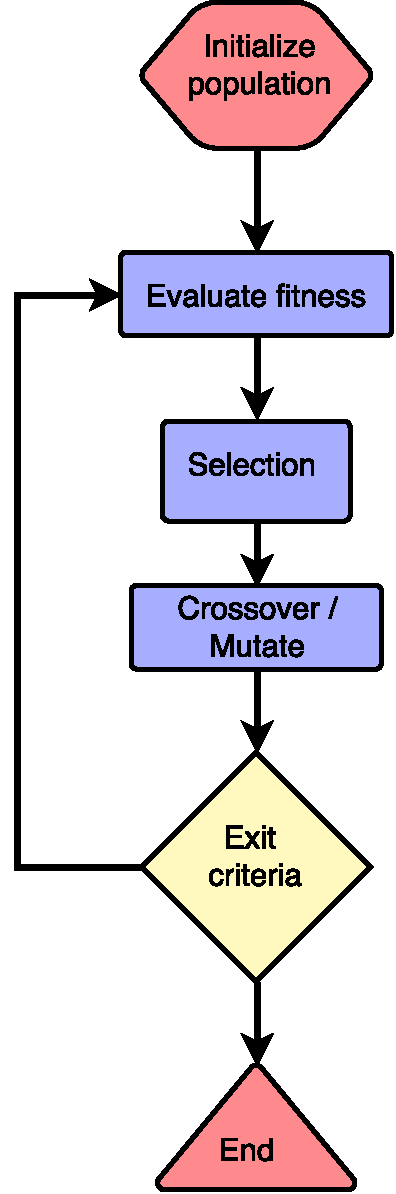
\includegraphics[width=\linewidth]{Chapters/Background/figures/ga_flowchart.pdf}
        %\caption{Genetic Algorithm}
    \end{subfigure}
    \hspace{0.25\textwidth}
    \begin{subfigure}[h]{0.25\linewidth}
        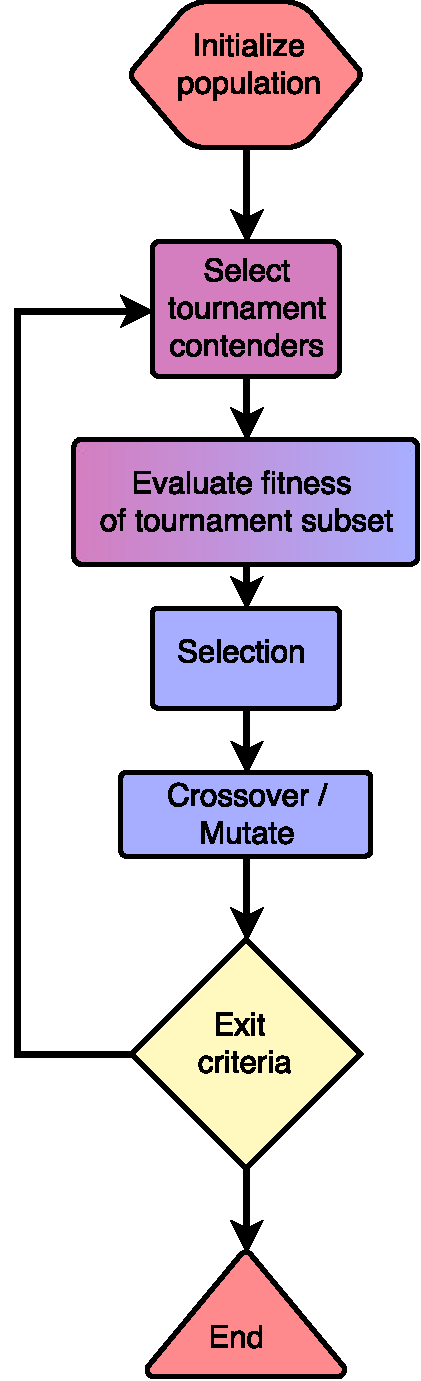
\includegraphics[width=\linewidth]{Chapters/Background/figures/tournamentsearch_flowchart.pdf}
        %\caption{Tournament Search}
    \end{subfigure}
    \caption{Flowcharts of the general Genetic Algorithm (left) and Tournament Search (right). The color blue indicates the operation is standard in a GA, while purple is special to a tournament search}
    \label{fig:algorithmflowcharts}
\end{figure}


\subsection{Tournament search}
One implementation of a genetic algorithm is the Tournament Search or Tournament selection. True to the name, every generation a subset of the population is selected for a tournament. The genotypes are evaluated with a fitness function and some selection scheme chooses genomes to be reinserted back into the population. The selection probability is given as 
\begin{equation}
    \label{eq:tournamentsearch}
    P_{i} = p(1-p)^{i-1}
\end{equation}
where i is the fitness-ranking achieved during the tournament (1 being first place and so on) and p the probability of choosing the winner to survive.  

In the search implementation used in the experiments in this thesis (see \ref{exp1:implementation} and \ref{exp2:implementation}), a version of the tournament search is used. For every generation, a selection of the total population given by the tournament size, is selected and evaluated. The winner then replaces each of the other contestants, making this implementation what is called a \textit{Deterministic Tournament Selection}, e.g: \(p=1\). Before the winner and its duplicate(s) is inserted back into the population, each copy of the winner is mutated under some probability to keep the diversity. 

A benefit of the tournament search, except for its efficiency in implementing and ability to work in parallel architectures, is that the \textit{selection pressure} of the search can easily be adjusted(see \ref{Search-experiment:Algorithms}). By increasing the tournament size, the winner of the tournament influence the future generations more.

\section{PathNet}\label{background:pn}
In 2017, DeepMind took the modular approach\footnote{Modular with respect to the traditional approaches of transfer from monolithic models} to deep transfer learning for multi-task systems one step further with their newly developed Super Neural Network structure\footnote{Super Neural Network are a meta-network where each node in the network is itself a Neural Network.}; \textit{PathNet}\cite{pathnet}. Where Progressive Neural Networks transfer knowledge between domains by adding a new uninitialized DNN for each task, the size of PathNet is not dynamic in the number of parameters. At training start, the net consists of randomly initialized weights in multiple DNNs, where each DNN is considered a module (or node) in a the larger PathNet structure. 

Using a combination of evolutionary and machine learning techniques, PathNet shares the PNNs traits of being able to optimize for multiple training tasks without catastrophic forgetting and transfer knowledge between tasks by reusing weights locked to backpropagation.  
\begin{figure}[h]
    \centering
    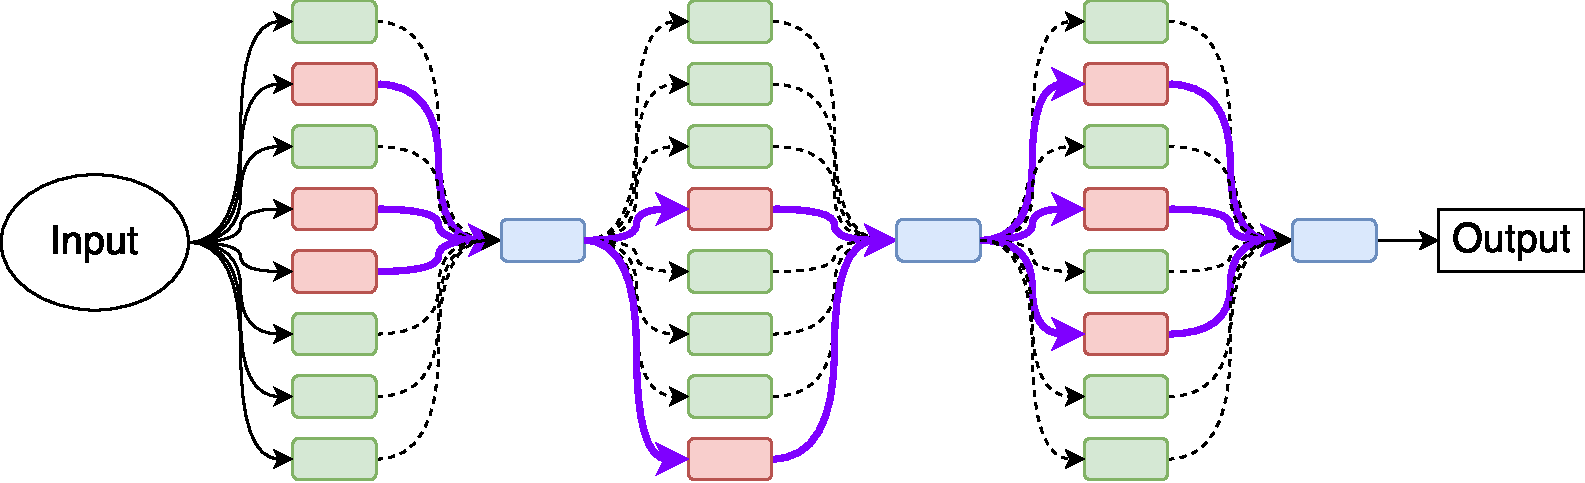
\includegraphics[width=0.8\textwidth]{Chapters/Background/figures/PathNet.pdf}
    \caption{Figure shows a PathNet implementation with 3 layers of 8 modules (NNs) in each layer. The \textit{red} color indicates the weights of this NN is locked to back propagation, while \textit{green} indicates it is open. \textit{Blue} cells are reduced-sum modules which summarizes the features between each layer. The purple connections show a path through the network. One path may use multiple modules from each layer, and may contain both locked and open modules.}
    \label{fig:pathnet}
\end{figure}

\subsection{Structure}
The PathNet consists of layers of modules, where each layer as a set number of modules as seen in figure \ref{fig:pathnet}. Each module is in itself a neural network of some sort, where the type of NN is adapted to the relevant task. Between each layer the output from each active module is passed through a reduced-sum operator that adds together each output element-wise to keep the dimensionality of the output from scaling by the number of active modules. 

Each task applied to PathNet is designated its own unique end-layer added to every path created for that task, meaning all paths in a search has the same final layer specific to that task. This layer defines the output and activation function to fit the problem at hand, be it classification, regression or something else.  

A \textit{path} is the name given a subset of the modules in a PathNet structure, where the path may contain between 1 and \(\omega\) modules from each layer, where \(\omega\) is adjusted to control the amount of capacity (number of weights) allocated to a path (solution). Each module in this path is locked after training is completed. This locking of the modules is to prevent the weights in the modules from changing if they are reused by subsequent tasks, and this preventative measure is what ensue catastrophic forgetting does not occur in this structure. After a optimal paths modules are locked, the rest of the modules that are not used in any path and does not contain optimized weights for a task is reinitialized. Fernando et al. claims\cite{pathnet} that this re-initialization is because they were not able to reach results that outperformed fine-tuning without it.

\subsection{Search}
For every new task introduced to the PathNet, a tournament search algorithm is initialized to find a optimal path through the network. A population of pathways (e.g: subsets of modules) are randomly initialized, and applied a tournament search with a tournament size of 2 and probability \(p=1\) of selecting the winner (as per equation \ref{eq:tournamentsearch}), making this tournament implementation deterministic. Every fitness evaluation of the tournament contenders is done by training them each a set amount and using the negative loss as a fitness value. The training amount is quite small at 50 batches of 16 examples each. This means that evaluating the fitness of a path changes the performance of that path, unless all modules in that path is locked to backpropagation.

When a winner is selected, the genome of the winner is duplicated to replace the looser and then mutated by each module in the path having a probability \(\frac{1}{L\omega}\) of being replaced with a neighbouring module\footnote{A module with index \(i\) is replaced with a module of index between \(i-2\) and \(i+2\)}, where L is the number of layers, and \(\omega\) is as mentioned the max number of active modules in each layer. The rather large mutation rate ensures that the average path, even if it contains the maximum number of modules, would have a genome change to separate it from the winner. Over multiple generations, however, the population converges to a lower diversity state where more and more paths contain similar modules. The search is terminated under some criteria, either a reached threshold fitness or a generation limit. 

\textbf{Edit note: More about pathnet needed? implementation details? Discussion about the experiments done in \cite{pathnet}?}

\section{Monte-Carlo probability estimation}
Given the nature of the systems used in this thesis, analytically calculating the probability of certain outcomes\footnote{In experiments \ref{exp1} and \ref{exp2}, the amount of module reuse for a random path selection is used as a comparison to experimental outcomes.} is quite hard. In such cases the probability of certain outcomes can be estimated with a Monte-Carlo approach. This is done by simulating some scenario governed by some stochastic properties for \(n\) number of trials and measuring some \(N\) number of outcomes. The probability \(p\) of these outcomes occurring can be estimated as 
\begin{equation*}
    \hat{p}=\frac{N}{n}
\end{equation*}
Since the error here is non-biased random with a mean error of zero, the standard deviation can be given as the square root of the mean squared error 
\begin{equation*}
    \sigma=\sqrt{E[(\hat{p}-p)^{2}]} =\sqrt{\frac{p(1-p)}{n}}
\end{equation*}


Selecting a sufficiently large \(n\) can be a problem with the Monte-Carlo approach since \(p\) is unknown. Still, we can for a fixed \(n\) select a maximum standard deviation we want and calculate the size of \(p\) at which point we lose accuracy. 

For a maximum ratio between the standard deviation \(\sigma\) and \(p\) of \(R\)\footnote{I.e: \(R=0.01\) means the probability of the measured outcome is 100 times larger than the standard deviation} and \(n\) being the number of trials, we can calculate maximum of \(p\) as
\begin{equation*}
    \frac{\sqrt{E[(\hat{p}-p)^{2}]}}{p} < R
\end{equation*}
\begin{equation*}
    \frac{1}{p}\sqrt{\frac{p(1-p)}{n}} < R
\end{equation*}
\begin{equation*}
    \frac{1-p}{np} < R^{2}
\end{equation*}
\begin{equation*}
    \frac{1}{p}< nR^{2}+1
\end{equation*}
\begin{equation}
    \frac{1}{nR^{2}+1}<p
    \label{eq:montecarloP}
\end{equation}
This means if we perform a Monte-Carlo simulation of \(10^{6}\) trials and we want the standard deviation to be at most \(0.01p\) the we lose certainty if the probability is smaller than \(\frac{1}{101}\).
\iffalse
    x   What is the required background knowledge? 
    x   Where can I find it? 
    x   What is the relevant prior work? 
    x   Where can I find it? 
    Why should it be done differently? 
    x   Has anyone attempted your approach previously? 
    x   Where is that work reported? 
    \Section{Nifty Gadgets my way}
    What is the outline of your way? 
    Have you published it before?  
\fi


\chapter{Implementation}
Machine Learning and especially Deep Learning systems are resource intensive algorithms that need large amounts of both training data and computations. Because of the nature of computations needed for machine learning typically is large matrix operations, it is preferable to run most of the training on GPUs.
\textbf{Edit note: Need more here}

\section{Python}
Python as a programming language choice for Machine Learning is becoming more and more common. Its strengths in rapid prototyping and large community that makes trouble-shooting easier is heavily out weighed by the slow run time, so while Python out-of-the-box is not suited for these operations, the number of good packages for machine learning and data-processing is quite good and works around Pythons native limitations. 

\subsection{TensorFlow}
TensorFlow\cite{tensorflow} is a open source symbolic math library. It is commonly used for Machine Learning and neural network implementation as it makes it possible for design of graph structures in \textit{Python}. The graphs created operate on n-dimensional matrices called tensors through graphs of mathematical operations, and is executed with low-level backend libraries such as \textit{C} or \textit{Fortran}.

TensorFlow also provides the support for different computing devices as needed, meaning the same implementation can be made to run on GPU with great benefits to computation time. The implementation in this thesis runs all model training (weight optimization) on the GPU, but because of the substantial computation performed on the CPU between each model training, the speedup from this is not as large as it could be. Future implementations could take advantage of customized graph-nodes to perform tournament searches quicker. 

\subsection{Keras}
Keras\cite{keras} is a high-level Machine Learning API that has a generalized and modular approach to neural network implementation. It depends on a specialized, well-optimized low-level backend library to perform necessary tensor operations and supports use of TensorFlow, Theano or CNTK backend. Keras provides a superior debugging feedback to a stand-alone TensorFlow implementation, while it supports micro-managing of parameters through tensors or matrices.

\begin{figure}[h]
    \centering
    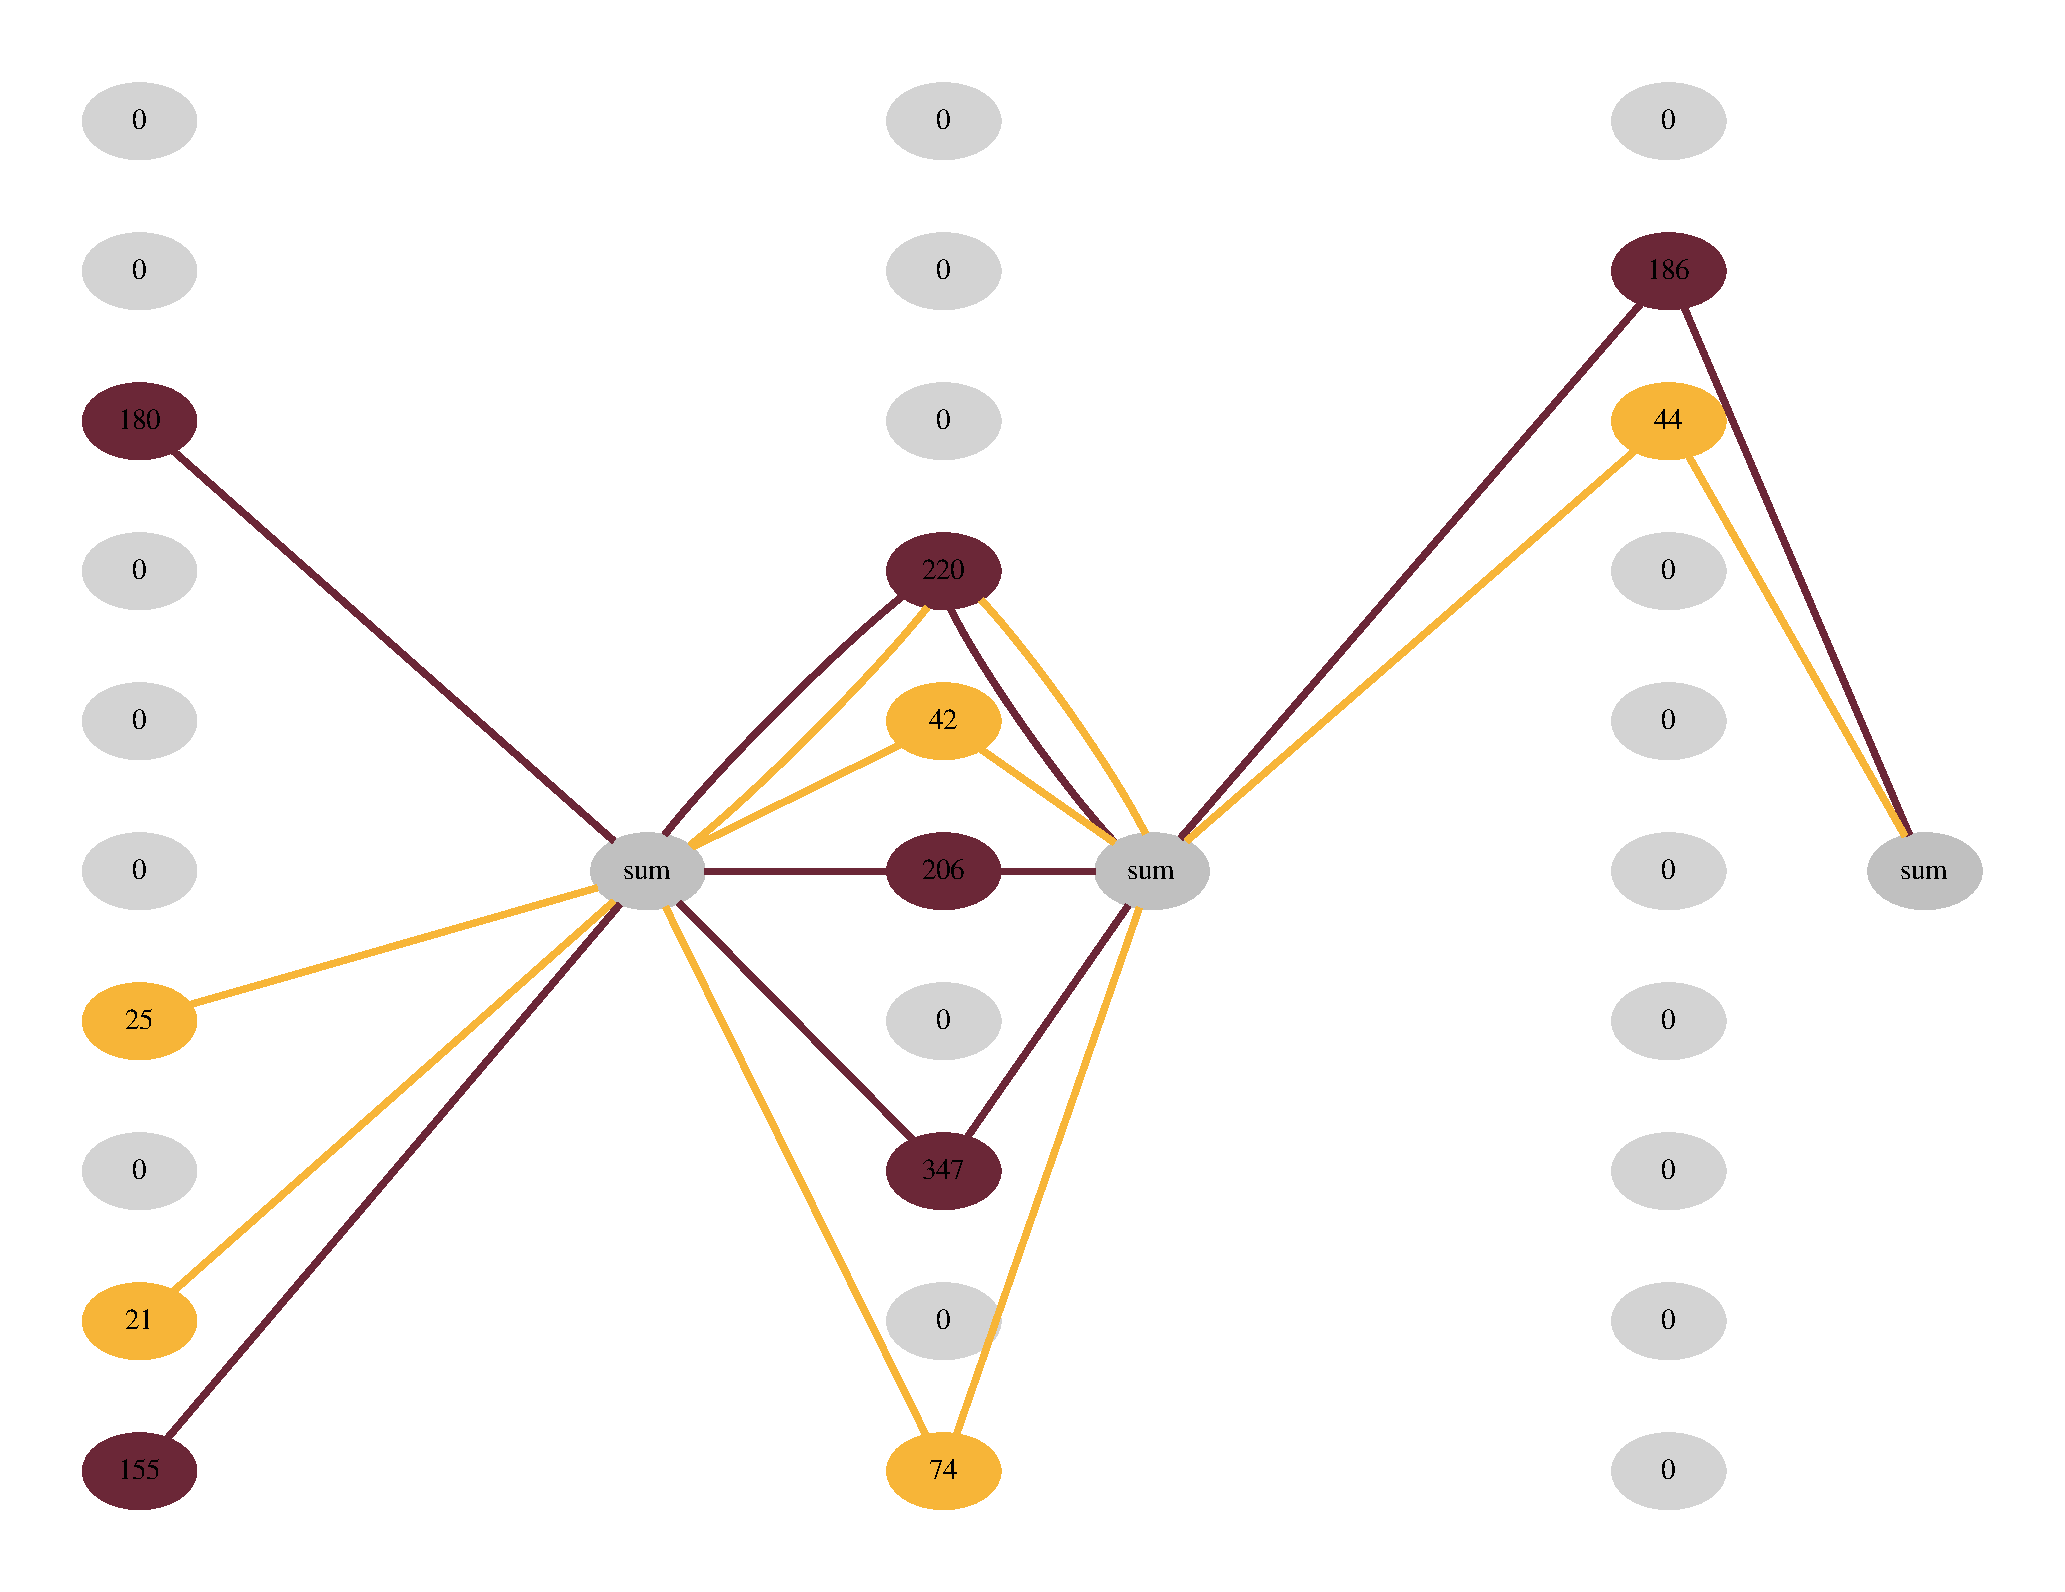
\includegraphics[width=0.8\textwidth]{Chapters/Implementation/figures/pathnet_visualization.pdf}
    \caption{Graph-visualization of a two optimal paths through a PathNet-structure created with GraphViz. This example is of a 3 layer PathNet with 10 modules in each layer. The first path (red) has a total of 6 modules and each module contain the number of training units that module have received. The second path (yellow) also use 6 modules, but reuse one module from the first path (second layer, fourth module from the top). Note that all modules not part of a path (gray) have undergone zero training because the weights have been reinitialized after finding the second path}
    \label{fig:pathnetexample}
\end{figure}

\subsection{Other packages}
Some other mentions to packages used during implementation of this thesis are
\begin{itemize}
    \item Pickle: Used during experimentation to store results and metrics.
    \item Matplotlib: Used for visualization of results.
    \item Numpy: Used for most mathematical operations not available through native Python functions 
    \item GraphViz: Used for generating graphs of PathNet structures for debugging. Multiple paths are drawn in same graph with training amount in each module as seen in figure \ref{fig:pathnetexample}
    \item Reprint: Used to manage search terminal output by refreshing multi-line output in the terminal.
\end{itemize}


\section{PathNet implementation}
As the same code is used in multiple experiments, it is built to be easily configurable and highly modular. This object-oriented design is based around Keras's already generalized approach to Machine Learning

\subsection{Code structure}
Modules are implemented through Layer-objects of two types: Dense layers to hold fully-connected modules and Conv layers to hold convolutional modules. Each module type is defined through a configuration-dictionary  describing the NN's that constitute a module. 

\begin{lstlisting}[language=Python]
    dense = [{'out': 20, 'activation': 'relu'}, 
             {'out': 5, 'activation': 'softmax'}]
    conv  = [{'channels': 10, 'kernel': (3,3), 
              'stride': (1,1), 'activation':'relu'}]
\end{lstlisting}
In the example above, the two lists yield different module-types. \textit{dense} defines a fully connected NN with two layers, where the first layer have 20 nodes with ReLU activation and the second have a softmax activation. \textit{conv} defines a one layer CNN where the two-dimensional convolution have 10 channels, use a three-by-three kernel with a stride\footnote{As mentioned in section \ref{background:ML}, stride is how far the kernel jumps in each dimension.} of 1 in each dimension and a ReLU activation.

The Layer-objects also define other operations that can be turned on or off on instantiation through parameters. These are:
\begin{itemize}
    \item BatchNormalization in Conv-modules. This normalizes the output from a layer within each batch. The reason for this is to average potential extremes/outliers in input examples to limit radical gradients during training. \textbf{Edit note: citation}
    \item MaxPooling used after last Conv-layer. This operation reduces the dimensionality of a layer output by reducing each x-by-y\footnote{Here, only MaxPooling of 2-by-2 windows are performed. This means a 10x10 feature map would be reduced to 5x5.} window of pixels to the max value within that window. \textbf{Edit note: citation}.
    \item Flatten before the first Dense-layer. This \textit{"housekeeping"} functionality takes some n-dimensional tensor input and flattens it to a vector to be input into a fully connected NN.  
\end{itemize}

As mentioned in \ref{background:pn}, each task has its own task specific final layer that defines the output from PathNet for that task. This final layer is defined through task-objects containing one layer of dully connected nodes, and a activation and size specific to each task. Here, only classification is done, so all tasks use a softmax activation. These object also contain some meta-info about the model they are a part of, such as input-dimensions, optimizer used for this task, a learning rate and loss function. 

Utilizing the layer and task objects are the PathNet object. Through hard-coded static methods a initialized PathNet structure is created for each experimental run. These methods initializes all layers, modules and configurations needed to start training. The PathNet-object also contain functionality for generating random paths and Keras-models from a given path and task object. It also contains a training counter for each module and interface for updating this value. There is also some \textit{housekeeping} functionality such as saving and locking modules after search and a TensorFlow-session backend reset (see section \ref{implementation:problems}).

\section{Search implementation}
As with PathNet the search have a modular implementation for easy adaptability and reuse in all experiments. Based around a hyper-parameter dictionary, the search method use predetermined functions for different GA operations such as selection-schemes for winner selection or path mutation. 

Every generation updates a Reprint-structure that gives terminal output of the search progress (see figure \ref{fig:searchoutput} for screen capture of a experimental run).
\begin{figure}[h]
    \centering
    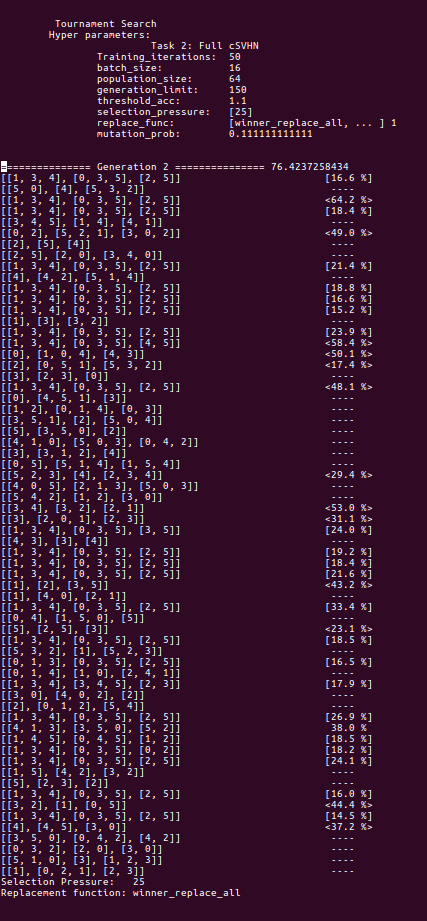
\includegraphics[width=0.6\textwidth]{Chapters/Implementation/figures/search_output.png}
    \caption{Screen shot of terminal output during a search. The top section contains hyper-parameters for this search as well as current generation number. Under neath the current population-state can be seen as well as some accuracies in the right margin. For these, \big[ \big] means the accuracy is outdated by training, \big< \big> means the value within is a training accuracy, .... means the path is not evaluated yet, and a plain percentage is the actual fitness of that path. At the bottom the current generations selection pressure as well as selection scheme is printed. }
    \label{fig:searchoutput}
\end{figure}
\textbf{Edit note: Need more?}

\section{Notable implementation differences}
\begin{itemize}
    \item Implementation is built upon the Keras API and is more modular in its object oriented structure
    \item Path fitness is not negative error but accuracy. 
    \item For the variable selection pressure experiment, the fitness calculation is performed after a separate training step. See \ref{exp2:implementation} for details and reasoning.
\end{itemize}

\section{Implementation difficulties}\label{implementation:problems}
Some implementation difficulties occurred during implementation. Most of these were due to TensorFlow effect I were unaware of. Some of the most noteworthy is listed here to help with future implementation
\begin{itemize}
    \item The TensorFlow backend session is not made for creating multiple graphs and memory leaks can happen when memory used for graphs is not freed properly. Functionality in TensorFlow makes it possible to reset a TensorFlow session, but all graph-variables has to be reinitialized afterwards. 
    \item TensorFlow's default is to use all available GPU-memory. Setting the TensorFlow-sessions GPU-options "allow-growth" parameter to 4 sets memory allocation to be done as needed.
    \item Allocated memory is not freed by TensorFlow until the Python process that initialized it is ended.
\end{itemize}

\iffalse
    X   Can you describe your implementation in detail? 
    X   Why did you use this technology? 
    X   How does the theory relate to your implementation? 
    X   What are your underlying assumptions? 
    X   What did you neglect and what simplifications have you made? 
    X   What tools and methods did you use? 
    X   Why use these tools and methods? 
\fi


\section{Data sets}
\subsection{MNIST}
One of the most commonly used data sets for image classification is the MNIST\cite{MNIST} set of hand-drawn digits. These 28 by 28 gray scale images contain one digit from 0 through 9 each. The 60 000  labeled images are distributed about evenly across all ten classes. 

\begin{figure}[p!]
    \centering
    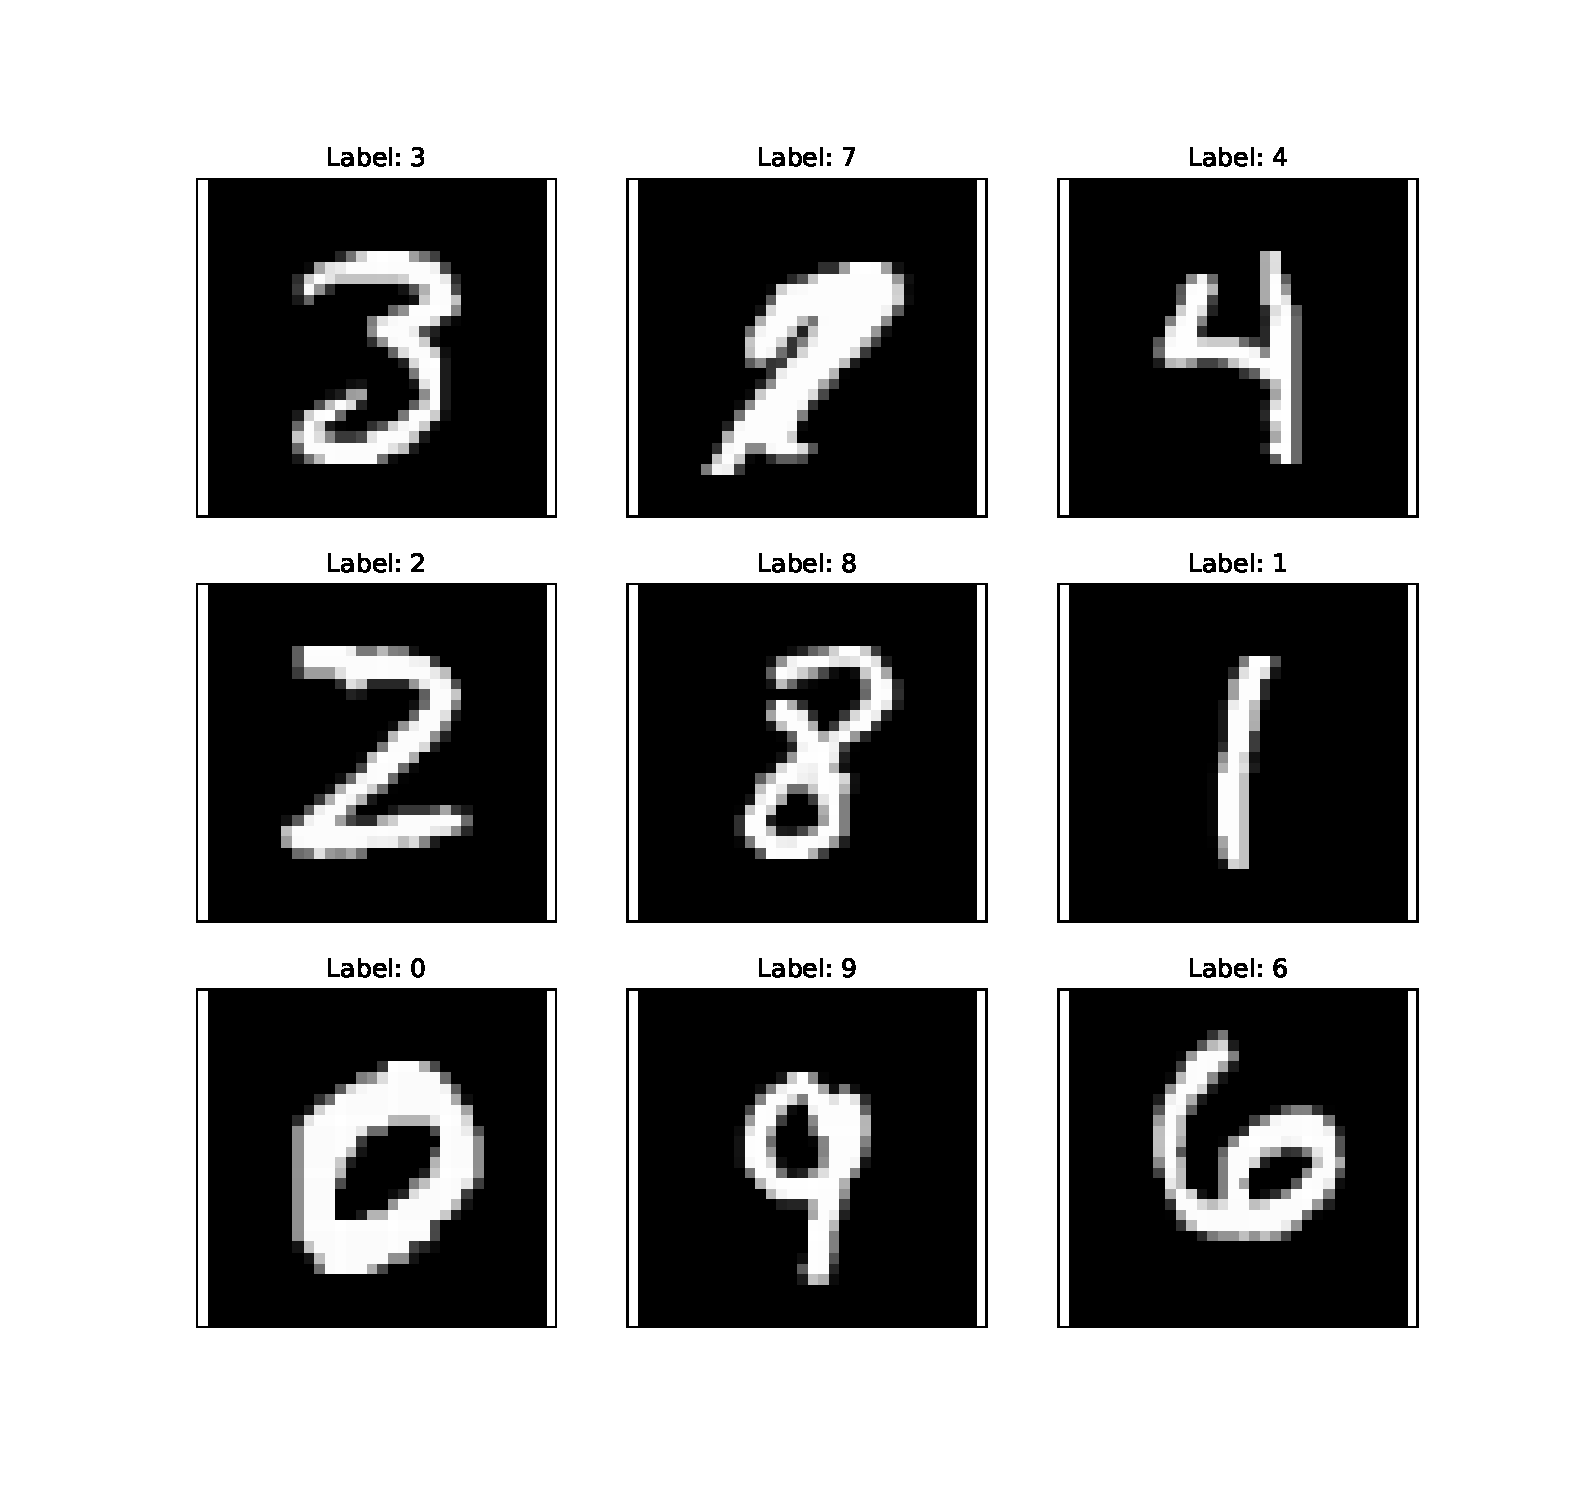
\includegraphics[width=0.8\textwidth]{Chapters/Implementation/figures/MNIST.pdf}
    \caption{Nine images from the MNIST data set.}
    \label{fig:mnist}
\end{figure}

MNIST is a simple data set as image classification goes (see section \ref{exp1:results.binary}). The gray scale small images contain only one small object in the middle of the image, and almost all pixels is either 0 (background) or 1 as seen in figure \ref{fig:mnist}. This makes the classification task rather easy. A list of reached accuracies\footnote{As of March 2018} can be found on the data sets web page where it is claimed that the lowest error rate is 0.23\cite{goodmnist}, and even a KNN-classifier without preprocessing can achieve an accuracy of 97.17. 


\subsection{SVHN}
The Street View House Number\cite{SVHN} data set is real world images from Google Street View made for machine learning development. The original data set contain over 600 000 variable resolution images of house numbers and bounding boxes around each digit with a label for each box. In this thesis, the version of SVHN used is made of cropped images (cSVHN) as seen in figure \ref{fig:csvhn}. These images are 32 by 32 colored images that are made to function in somewhat the same way MNIST does with a simple object and static size. Note however, that where MNIST images contain only the object that is the basis for classification, cSVHN contain distractions (noise) in the image such as half-cropped other digits. 

\begin{figure}[p!]
    \centering
    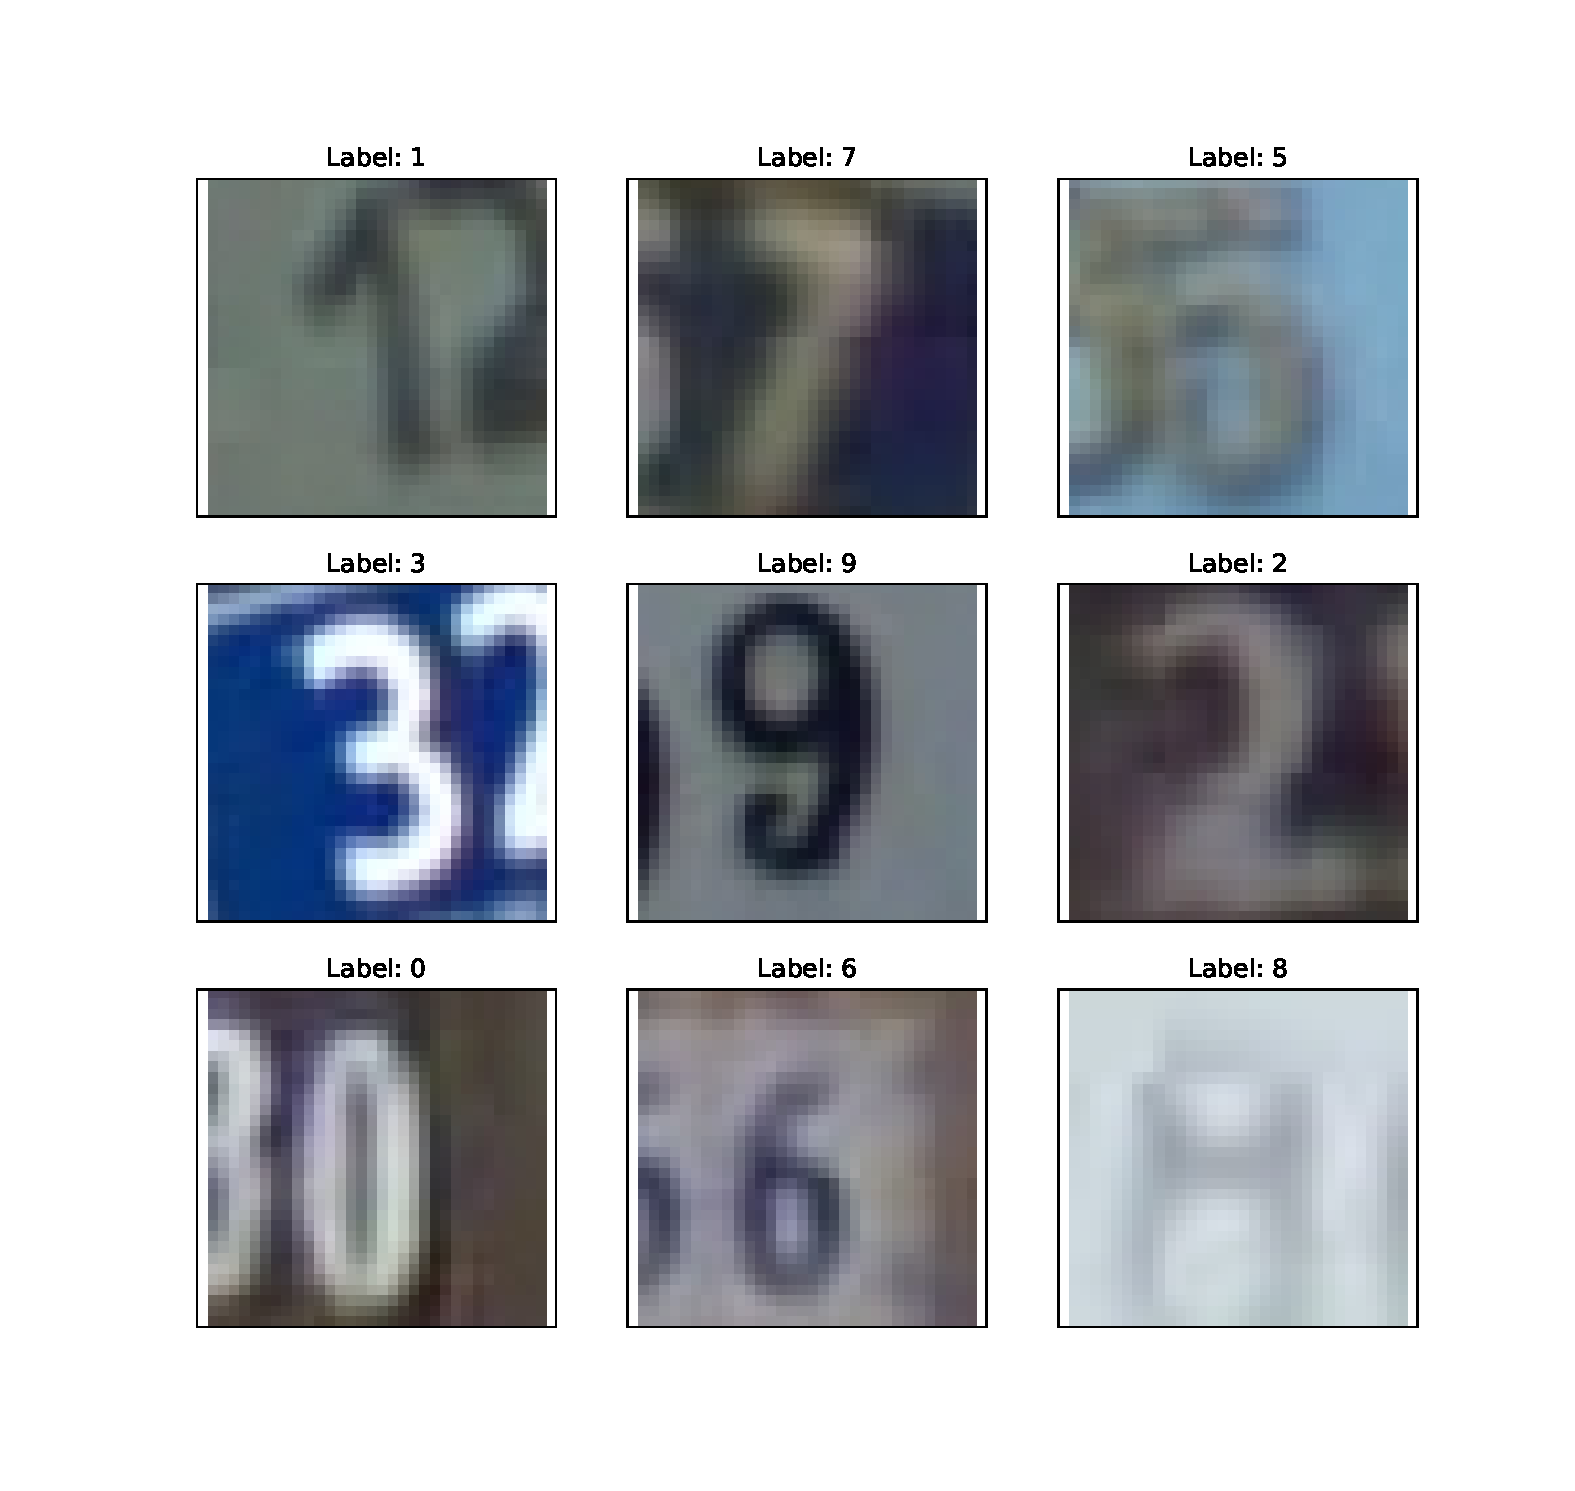
\includegraphics[width=0.8\textwidth]{Chapters/Implementation/figures/cSVHN.pdf}
    \caption{Nine images from the cSVHN data set.}
    \label{fig:csvhn}
\end{figure}

The whole image set is split in three sets, a training set containing 73257 digits, a test set of 26032 digits, and a simplified \textit{"extra"} image set of 531131 images, claimed by the creator to be "less difficult". This extra, simplified image set is the one used in experiments \ref{exp2} for task 3a, 3b and 4.

\begin{table}[h]
    \label{tab:SVHN}
    \centering
    \begin{tabular}{ccc}
    Class number (Digit) & Number of samples & \% of whole data set\\
    0                    & 45550             & 8.6\%               \\
    1                    & 90560             & 17.0\%              \\
    2                    & 74740             & 14.1\%              \\
    3                    & 60765             & 11.5\%              \\
    4                    & 50633             & 9.5\%               \\
    5                    & 53490             & 10.1\%              \\
    6                    & 41582             & 7.8\%               \\
    7                    & 43997             & 8.3\%               \\
    8                    & 35358             & 6.7\%               \\
    9                    & 34456             & 6.5\%              
    \end{tabular}
    \caption{Distribution of samples on each class in the cropped SVHN set used in this thesis, along with the portion of the whole set each class constitute. Given a random selection of samples from this set, this percentage should approximately be the probability of selection each class}
\end{table} 

Because these images are from the real world, and because of the nature of house numbers, the class distribution is not even. In table \ref{tab:SVHN} the number of digits in each class in the extra set is listed along with the portion of the whole set this constitutes.  


\chapter{Experiment 1: Selection versus search}\label{exp2}
Disregarding what algorithm is used during path searching, training multiple machine learning models are usually rather resource intensive. In the case of training subsets of a Super Neural Network, even more so. Any small reduction in the computation time here will pay off in the long run, especially during experimentation where multiple iterations of PathNet training are going to be preformed. Keeping this motivation in mind, the first experiment I preformed is one where the results either confirm a shortcut in experimentation can safely be made, or will give some insight into the layer interface of a model when applying different training schemes.

The questions I want to answer is simple: \textit{Is there anything to gain from performing a proper search for the first path versus just picking a random path and training those weights using a classic end-to-end training scheme?}

\section{Hypothesis}
It is self evident that picking a random path and training that subset of weights end-to-end will be more computationally efficient than a full search through a population of possible paths. A full search in a newly initialized PathNet means we are looking for modules with the most appropriate initial weights, which is a lot of labour for a rather small amount of reward. If proven not to affect the reuse of modules between tasks, end-to-end training of a random path means there is nothing to gain from this labour. In this case the following experiments will be done with a random selection of the first path. 
%SHOW HOW MUCH OF TRAINING DURING A SEARCH IS ACTUALLY USED BY OPTIMAL PATH VS. WEIGHTS THAT ARE REINITIALIZED
What I suspect is that end-to-end training will cause the modules in the randomly chosen path to have a highly codependent interface between modules. This might then make it harder for subsequent tasks to reuse the intertwined modules, and make the encoded knowledge in those modules more task specific than in the case of a full path-search. 

When training on two tasks, the amount of module reuse between these tasks should be lower when we end-to-end train a randomly chosen path. To prove this, the following experiment is suggested. 

\section{Description}
The experiments in this section is divided in two parts. 
\begin{itemize}
    \item Search + Search (S+S): A full search for task A is performed on a newly initialized PathNet. The optimal path is saved and locked as per the PathNet design, then another full search for task B is performed.
    \item Pick + Search (P+S): A path is selected from the PathNet modules and trained on task A with a classic end-to-end training scheme. This path is then saved and locked normally. Then a full search is done for task B.
\end{itemize}
Performing multiple runs of this experiment should show a trend in module reuse between S+S and P+S scenarios. To ensure that the first path in P+S does not have an advantage or disadvantage in total capacity,  the path found for task A in S+S is stored and used as the randomly chosen path for task A in the P+S scenario.
This ensures that when training on task B in both the S+S and P+S scenario, the only difference is the weights along the path for task A, and the way these were reached. 

As data set for task A and B, I chose the MNIST set of handwritten digits. This is because of the task simplicity and availability of the data set and it is the same initial experiment DeepMind did in their original paper on PathNet, the difference being the addition of salt and pepper noise to the data to increase the difficulty of the task.

I performed two experiments of this type. First a binary classification scenario where I selected four classes from the ten available in the MNIST set and split them into two groups of two classes as task A and task B. The second experiment was a quinary classification scenario where all 10 classes were used in two groups of five each. The reason for the second experiment is discussed in the result section of experiment one. 

\section{Implementation}\label{exp1:implementation}
The implementation of PathNet have already been described in a preceding section of this thesis, so only hyper-parameters used in the experiment will be discussed here.

\begin{table}[]
\centering
\begin{tabular}{lll}
Experiment             & Binary MNIST                                                                                 & Quinary MNIST                                                                                                                                                     \\
Number of Layers       & 3                                                                                            & 3                                                                                                                                                                 \\
Number of Modules      & 10                                                                                           & 10                                                                                                                                                                \\
Module structure       & Dense only                                                                                   & Dense and Conv                                                                                                                                                    \\
Maximum active modules & 3                                                                                            & 3                                                                                                                                                                 \\
PathNet structure      & \begin{tabular}[c]{@{}l@{}}Flatten \\ Dense\\ Dense\\ Dense\\ Unique /w softmax\end{tabular} & \begin{tabular}[c]{@{}l@{}}Conv + BatchNormalization\\ Conv + BatchNormalization\\ Conv + BatchNormalization\\ Maxpool\\ Flatten\\ Unique /w softmax\end{tabular} \\
Task optimizer         & SGD                                                                                          & Adam                                                                                                                                                              \\
Learning rate          & 0.0001                                                                                       & 0.0001                                                                                                                                                            \\
Loss function          & Binary Crossentropy                                                                          & Categorical Crossentropy                                                                                                                                         
\end{tabular}
\caption{Hyperparameters used in the first-path experiments. A Dense module here consists of 20 fully connected nodes with ReLU activation, while a convolutional module is 1 channel of a 3-by-3 kernel with 1-by-1 stride and ReLU activation.}
\label{tab:hyperparam}
\end{table}

\subsection{Binary MNIST classification}
A similar PathNet structure to the MNIST experiment in the original PathNet paper is used here. 
Three layers with a maximum of three active modules from a total of 10, each with 10 fully connected nodes followed by ReLU-activation. Since each data point in MNIST is a 28 by 28 gray scale picture, the matrix of input-values is first flattened to a 784-element vector before it is used in training. The digits 3 and 4 were selected as task A, and digits 1 and 2 as task B. 
During the search, a population of 64 paths were used, and the search halted when a training accuracy of 98\% were reached, or after 500 generations. During tests, searches that exceeded 500 generations usually persisted for more than 1000 generations because the training was stuck in a local-minima. The population had always converged to one path at that point, and excessive training on a converged path would after a while approximate end-to-end training. Because of this and limitations to available experimentation time, the limit of 500 generations were enforced. The task specific classification layer that is used alongside the PathNet weights is obviously restricted by the training scenario and its use, so it consists of two fully connected nodes followed by Softmax-activation for the purpose of classification.
A total of 600 experimental runs were performed.

\subsection{Quinary MNIST classification}
A different PathNet structure was implemented here. The first two layers consisted of 10 convolutional modules each, where a convolutional module contained two convolutional layers, the first with a 3 by 3 kernel and ReLU activation, and the second with a 5 by 5 kernel and ReLU activation. Following these convolutions, a Bach Normalization layer were added to reduce the spread in gradients. The third and last PathNet-layer were 10 modules of 20 fully connected nodes and another ReLU activation. To connect the second and third layer, a two dimensional maxpooling reduced the dimensionality of the second layers output before the 2D matrix were flattened to a vector.   

The path searches were again done with a population of 64 paths and a limitation of 500 generations, but the threshold training accuracy used here were 97.5\% to limit run time. 
Since the classification task here were quinary and all 10 classes from the MNIST set were used, for simplicity's sake, task A consisted of digits 0 through 4, and digits 5 through 9 made up task B. 

This experiment were considerably more computationally expensive to run, so it was programmed to keep running until no more time could be dedicated to this experiment. In the end, this ended up being 535 experiments. 



\section{Results}
\subsection{Binary MNIST classification}\label{exp1:results.binary}

\begin{figure}[t]
    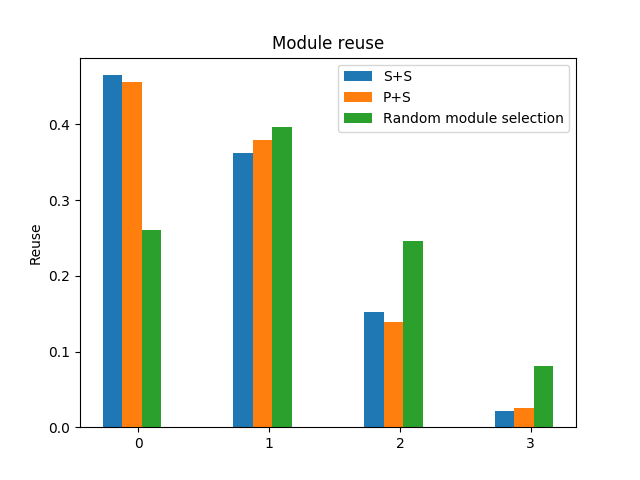
\includegraphics[width=\textwidth]{Chapters/Experiments/first_path/figures/600binMNIST_module_reuse_histogram.png}
    \caption{Distribution of module reuse in S+S and P+S searches alongside expected module reuse for random selection of modules in first and second task[green]. This plot is a result of 600 experimental runs.}
    \label{fig:binMNIST.hist}
\end{figure}

For ease of comparison, four plots are automatically generated in both experiments. These visualize the amount of module reuse alongside different metrics such as average training or frequency counts. 
The most intuitive of which is the module reuse bar graph in \ref{fig:binMNIST.hist}. The hypothesis would manifest itself in this plot as a significantly higher blue bar for higher number of reuse compared to the orange bar of P+S. Instead, no difference in reuse for the two scenarios can be seen. Another observation from the figure is that the frequency of modules with no reuse at all is around 66\% higher than the frequency of zero reuse when randomly selecting modules for two paths. This could indicate that training new modules from scratch is simpler for the model than adapting to interface of previously used weights.

These observations differ from our hypothesis that end-to-end training causes confounded interfaces between layers, but this could be caused by the task we are trying to solve being too simple. This again would cause the paths to train very little and the available capacity in the paths to be too high. When the distance in parameter space between initialize parameters and "good enough" parameters are too small, the gain from reusing modules can not be justified. In other words, learning the task \textit{de novo} is simpler than learning the interface-quirks of a preceding previously used module.

\begin{figure}[t]
    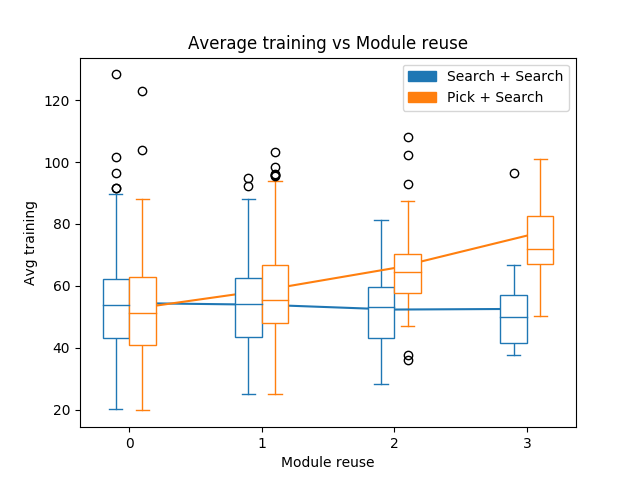
\includegraphics[width=\textwidth]{Chapters/Experiments/first_path/figures/600binMNIST_training_boxplot.png}
    \caption{Box-plot depicting average amount of training each module within a path gets for each group of module reuse for both P+S and S+S. }
    \label{fig:binMNIST.box}
\end{figure}

We find support for this claim in \ref{fig:binMNIST.box}, where a clear upwards trend in the average training can be found for P+S, while there does not seem to be a change for S+S. This could mean that in order to reach the same accuracy threshold as S+S, P+S has to undergo more training, meaning the interface between modules is more complicated i P+S than S+S. Please note that the subsets of models with module reuse of 3 is quite small. \ref{fig:binMNIST.hist} visualizes this difference in group size quite well.

The last plot in \ref{fig:binMNIST.layer_reuse} shows something unexpected. The results for search+search and pick+search indicate the same as \ref{fig:binMNIST.hist}, no significant difference in the module reuse. But here, the reuse is shown for each layer in the models. The first layer have significantly lower reuse than the second two. This is the opposite of what we would expect based on the conclusion made by Yosinski et al\cite{yosinski2014transferable}, where the first layers tended to be the most general and easily reusable. This is most likely a property of using multi-layer perceptrons as modules and would disappear if the modules in question consisted of convolutional operations. Fully connected NNs are poor at generalizing to image data because of images complex class manifolds, and as a result of the raw image processing most CNNs end up performing in their first layers, convolutional layers that approximate Gabor-filters ends up being highly transferable.

What we see instead is that most module reuse happens in later layers in the PathNet. It is hard to tell exactly why this is, but a possible explanation is that a path contains more capacity than it needs and the later layers are capable of doing all the heavy lifting. In that case the first layer does not contain use full weights, and therefore there is no incentive to reuse those modules. 

\begin{figure}[t]
    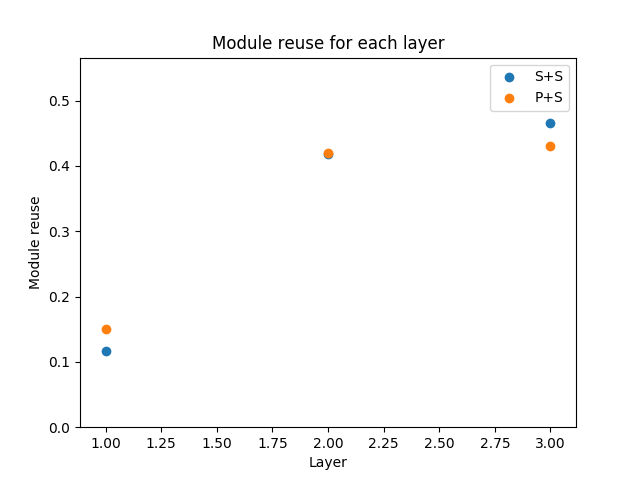
\includegraphics[width=\textwidth]{Chapters/Experiments/first_path/figures/600binMNIST_reuse_by_layer.png}
    \caption{This plot shows how the total amount of reuse in all experiments are distributed on the three layers in the PathNet structure }
    \label{fig:binMNIST.layer_reuse}
\end{figure}

Since this implementation is one of fully connected nodes, each neuron have to generalize to its corresponding image pixels, and would therefore be highly task specific. This is the motivation behind performing the quinary MNIST classification experiment in addition to this one. More classes constitute a "harder" classification task, and the change from NNs to CNNs as modules should remove some of the effects we have seen in the plots in this section. Effects we hope to see in Quinary MNIST classification is

\begin{enumerate}
    \item A separation between P+S and S+S in frequency of models with a higher module reuse.
    \item S+S should have a frequency distribution closer to the distribution by randomly choosing modules.
    \item A significantly smaller divergence between P+S and S+S in average training for each module reuse group. 
    \item A more even distribution of module reuse on each layer in a path.
\end{enumerate}


Point 4 because the modules are changed from NNs to CNNs, and 1 through 3 because we increase the task difficulty and therefore also the necessary training time. 

\subsection{Quinary MNIST classification}

\begin{figure}[t]
    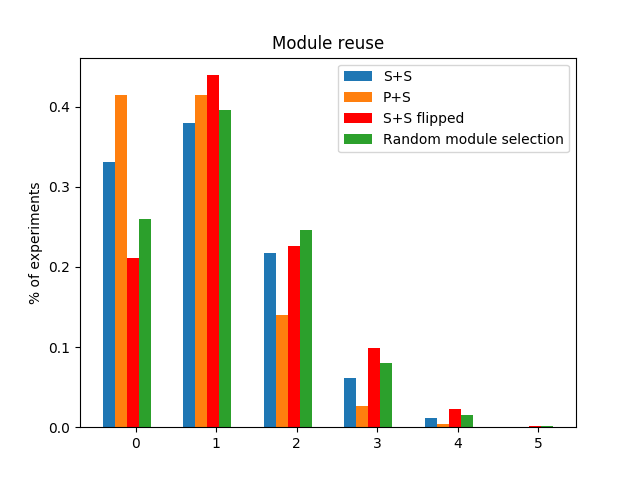
\includegraphics[width=\textwidth]{Chapters/Experiments/first_path/figures/535MNIST_module_reuse.png}
    \caption{Frequency histogram equivalent to \ref{fig:binMNIST.hist} for the Quinary MNIST classification experiment. The red bar shows reuse in a training scenario similar to S+S, but where the order of tasks is reversed.}
    \label{fig:quinMNIST.hist}
\end{figure}

\begin{figure}[t]
    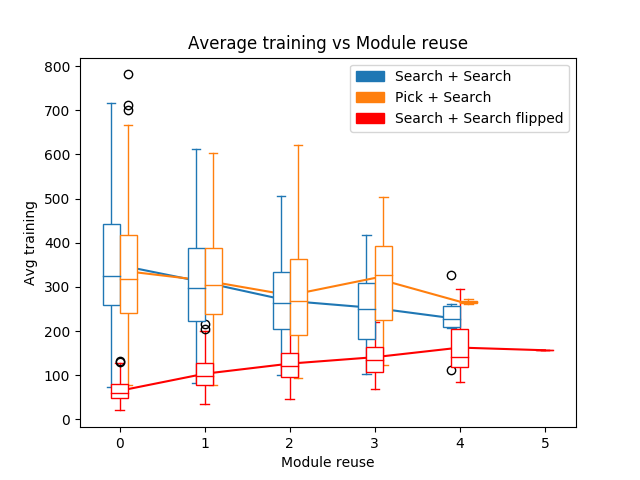
\includegraphics[width=\textwidth]{Chapters/Experiments/first_path/figures/535MNIST_training_boxplot.png}
    \caption{Average training box-plot equivalent to \ref{fig:binMNIST.box} except for the addition of a training scenario similar to S+S but where the task order is reversed}
    \label{fig:quinMNIST.box}
\end{figure}

\begin{figure}[t]
    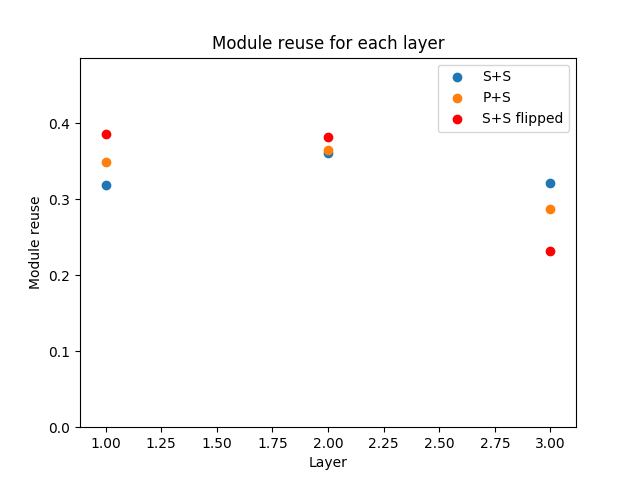
\includegraphics[width=\textwidth]{Chapters/Experiments/first_path/figures/535MNIST_reuse_by_layer.png}
    \caption{Frequency of module reuse for each layer in the paths. Equivalent to \ref{fig:binMNIST.layer_reuse} except for the addition of a training scenario similar to S+S but where the task order is reversed}
    \label{fig:quinMNIST.layer_reuse}
\end{figure}


It is quickly eminent from figures \ref{fig:quinMNIST.hist} and \ref{fig:quinMNIST.box} that the increase in task difficulty between binary MNIST and quinary MNIST have uncovered effects predicted in the original hypothesis. In the bar graph \ref{fig:quinMNIST.hist}, the amount of reuse in S+S and P+S have separated, and even though this is not conclusive evidence of the interface confounding predicted, the effect shown here is strong enough to discourage the end-to-end training of a chosen first path. We also see confirmation of point 2 in the list of predictions made in the previous section of this thesis. 

In \ref{fig:quinMNIST.box} the divergence between S+S and P+S for the higher levels of reuse have disappeared, and now a downwards trend in average training is emerging. Recall the point made earlier that the later boxes in this figure represent a significantly smaller group compared to those of less reuse (see \ref{fig:quinMNIST.hist}), but there still looks to be a decline in average training when the amount of reuse within a path increase. This effect can be explained if we suspect the task used for the first path in each experiment to be easier than the second. 

Say task A in a two task system is much simpler than task B. After optimal path for task A have been found and locked, the PathNet will consist of most modules with no training, while those along path A will have a small amount. If task B is harder and more training is done during the search for path B, more reuse of modules means a higher amount of modules in path B have been trained during task A and therefore have received less training in total. The average amount of training for task B will then be lower for higher levels of reuse. 
The opposite will be true if task A is harder than task B. More reuse of modules with more training means the average training for task B will go up for higher levels of reuse. 

The red boxes in figure \ref{fig:quinMNIST.box} confirm this. This part of the plot is from a training scenario similar to Search + Search, but where the order of tasks is reversed\footnote{In S+S, task A consisted of classifying the classes \{0, 1, 2, 3, 4\}, while task B were classes \{5, 6, 7, 8, 9\}}. We see a clear upwards trend in the groupings but also note the average training for each level of module reuse is lower in the flipped S+S scenario.
%WHY!?
In figure \ref{fig:quinMNIST.hist}, the amount of paths with no module reuse in the flipped S+S scenario is half of P+S, which means it has a all around higher module reuse. I previously discussed the fact that the probability of having no reuse is higher for these training scenarios than that of a random module selection, but this is not true for flipped S+S. 
It seems the experiment is simplified by training on the hardest task first. Another experiment should be run to see if this holds true for flipped P+S training.

In figure \ref{fig:quinMNIST.layer_reuse} the difference between S+S and P+S is more significant, and we can also see point 4 in the list of suspected changes confirmed. Reuse is more evenly distributed across the layers. For flipped S+S we can see what we originally expected from this plot, that the level of reuse is higher for the first layers and then decline as the abstraction in each layer increase. 

\section{Conclusion}
In conclusion, results in quinary MNIST classification as well as the comparison with the binary MNIST experiment show promising, if not conclusive, evidence of end-to-end training causing confounded interfaces between modules and a reduction in transferability between task in a multitask scenario. Note should also be taken of how task difficulty effect reuse, and ordering of task from low difficulty and upwards will manifest as a lower average training for paths with a high level of reuse. Results in figure \ref{fig:quinMNIST.hist} tells us there is something undiscovered and unexpected hidden in the ordering of tasks, and further experiments is called for to  uncover this. 

Motivation for these experiments were the possibility of reducing experimentation time by not searching for the first path in the PathNet structure, but the reduction in transferability is dissuading enough to not justify forgoing a full search for all paths. 


\chapter{Experiment 2: Selection pressure}\label{exp2}
In the original paper, Fernando et al. used a tournament search algorithm for path optimization. This algorithm was selected on the basis that it fills the role of simplest possible 'agent' for path-selection, one which can be considered a unit of evolution.  The tournament implementation fits this description as a 'unit' because of the tournament size used. Within one generation, the total change in the population is one genotype being replaced with another from the same population and subjected to mutation under some probability. Building on the previous set of experiments where the conclusion can take form as an argument in favour of a high exploration rate during path-search, we would expect a tournament of size two to yield modules with high transferability and a high number of reuse compared to a high tournament size. In these experiments, this will be tested by manipulating the selection pressure during the tournament search. Questions addressed in this section is: 
\begin{itemize}
    \item How would different evolutionary algorithms influence outcomes in training a PathNet structure on multiple tasks?
    \item What evolutionary strategies make the most sense in the scheme of training an SNN?
    \item How would a changing selection pressure affect learning? 
\end{itemize}

\section{Description}\label{Search-datasets}
\subsection{Data-sets} \label{exp2:datasets}
To address these questions a trial of different searches have been applied to a PathNet structure for a selection of tasks. As with the first-path experiments, the search algorithms will be applied to image classification tasks. Building on what we learned with regards to task difficulty, two different data-sets have been selected, and the different tasks will be derived from this data. The tasks will be ordered by assumed difficulty to follow a gradual learning mentality. 


\begin{enumerate}
    \item MNIST subtasks
    \begin{enumerate}
        \item Digits 0, 1, 2, 3 and 4
        \item Digits 5, 6, 7, 8 and 9 
    \end{enumerate}
    \item Full MNIST classification
    \item Cropped SVHN subtasks
    \begin{enumerate}
        \item Digits 0, 1, 2, 3 and 4
        \item Digits 5, 6, 7, 8 and 9 
    \end{enumerate}
    \item Full cSVHN classification
\end{enumerate}

It was shown during the first-path experiments that task 1a and 1b is not of the same difficulty level, however, within this context we will consider the training amount needed to reach a satisfactory accuracy level is similar enough for these tasks to be grouped together. The natural progression from a full MNIST classification to a SVHN is thought to increase the incentive for module reuse, even if the SVHN task will have to learn to ignore distractions in the images (see \ref{section:Datasets.SVHN}) that the MNIST classifiers does not have to deal with. The difference in image-dimensions have been addressed in \ref{exp2:implementation}.

As mentioned in \ref{section:Datasets.SVHN} there are two formats to the SVHN set, one of variable image resolutions, and one that mimic the MNIST set in static square size called cropped SVHN (cSVHN). cSVHN is selected for these experiments in order to use a constant input size to the PathNet. Within the larger set of cSVHN images, a subset described as containing "somewhat less difficult samples" is used. To increase the number of tasks, the rest of the data in SVHN could be used and noise could be added to the images to increase the task difficulty artificially. 

For both the MNIST and cSVHN set, the amount of training data have been limited to 10000 training samples and 4000 validation samples. Of these samples, MNIST have an fairly even distribution on each class while SVHN have an imbalance in the class distribution. Since the samples used are randomly selected before each experimental run, the probability of select one sample from a given class can be derived from the total amount of samples in that class (see \ref{section:Datasets.SVHN} for the exact number of samples in each class).

Each experimental run will apply a searching scheme to find an optimal path in a gradually increasing knowledge base within a PathNet. This means, for instance, tasks 1a always will be learned in a module set of only initialized weights and no previous knowledge. It is assumed that with a different ordering in tasks, other  accuracy and training results would have been reached, but as this tells us more about the tasks selected than it does about the search algorithms used, and as each experimental run is significantly more time consuming than in the first-path experiments, this will not be attempted here. It is considered that this reversing of subtasks within a data-set partition could be used as an simple, if time consuming and crude data analysis tool.

\subsection{Algorithms}\label{Search-experiment:Algorithms}
The different versions of tournament search explored here have been divided into three groups: 
\begin{enumerate}
    \item Constant selection pressure
    \begin{enumerate}
        \item Tournament size 2
        \item Tournament size 25
        \item Tournament size 3 + recombination
    \end{enumerate}
    \item Scaling selection pressure
    \begin{enumerate}
        \item Low to high pressure: 2, 5, 10, 15, 20, 25
        \item High to low pressure: 25, 20, 15, 10, 5, 2
    \end{enumerate}
    \item Dynamic selection pressure
    \begin{enumerate}
        \item Gradual change from 2 to 25 over all generations
        \item Gradual change from 25 to 2 over all generations
    \end{enumerate}
\end{enumerate}
In total, the seven tournament algorithms are used 10 times each within a reinitialized PathNet structure to train on all tasks discussed in \ref{Search-experiment:Datasets}. Between algorithms, the only hyper-parameter change is the tournament size and replacement method within each tournament. All algorithms except 1c use a winner-replace-all scheme where the mutation of the strongest paths genome replaces each of the loosing contenders in the tournament. In algorithm 1c, three contenders are selected randomly from the population and evaluated. The two strongest genomes are labeled as parents and (starting with the winner) takes turns copying their layers to the offspring. The offspring is then subject to some mutation under the same probability as every other algorithm, and replaces the loosing genome in the tournament.
\begin{figure}[h]
    \centering
    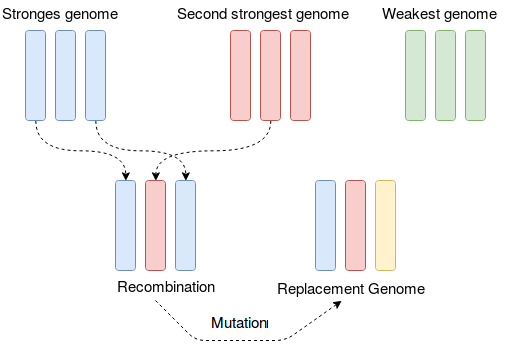
\includegraphics[width=0.8\textwidth]{Chapters/Experiments/search_algo/figures/Recombination_algorithm.png}
    \caption{Visualization of the recombination in algorithm 1c. In a three layer PathNet, the first and last layer in the recombination would be layer one and three in the winning genome, while layer two would stem from the second strongest genome. After a mutation of the recombination, the new genome replaces the loosing contender. Each color represents one genome from the tournament and yellow represents a mutation.}
    \label{fig:search.recombination_algorithm}
\end{figure}

Algorithm group 2 consists of two algorithms where the tournament size is changed between each task. This means algorithm 2a uses tournament size 2 for task 1a, task 1b uses tournament size 5 and so on until the last task of full cSVHN classification which uses tournament size 25. In algorithm 2b, this order of tournament sizes is reversed. It is expected that in visualization of metrics where a population average is calculated for each generation, such as training accuracy, an algorithm with high selection pressure will have abrupt value changes from one generation to the next. Low selection pressure would then give a more gradual change in such values. A change between these two curve types should be prominent for algorithms 2a and 2b.

Algorithms 3a and 3b have its selection pressure changed during each tournament search. This means each algorithm behave the same for each task, which algorithms 2a and 2b did not. The change in selection pressure is gradual which means between tournament sizes 2 and 25, each tournament size is used about 4 times for a search termination limit of 100 generations. It is obvious that an even distribution of tournament sizes on each generation is not possible when using a threshold accuracy as search termination, which is one reason searches in these experiments are limited by number of generations instead. 

\subsection{Metrics}\label{Search-experiment:Metrics}
Due to the experiment complexity and number of tunable hyperparameters there are a large number of search effects and attributes that could be investigated, so limitations have been introduced on which metrics are being addressed. 

As with the first-path experiments, module reuse between tasks will be an important metric. This number is highly effected by stochastic processes such as initialization of populations, mutation probability, layer sizes, path sizes and so on, but it is also the most intuitive and clear way to measure the transferability of module knowledge. An assumption used behind this metric is that modules are able to contain some form of "memetic"\footnote{Memetic is used here to describe a quantification of knowledge in the same way "meme" is used by Richard Dawkins\cite{selfishGene} to describe a unit of cultural knowledge} unit knowledge. In this multi-task scenario, reuse can occur across multiple tasks, but focus will here be put on the total number of modules reused instead of separating the reuse across tasks. This is because any effect algorithm choice has on module reuse will be compounded and easier to spot in the total amount of reuse rather than in reuse between tasks.
%ABRIDGED: This is because if the effect on reuse between each search algorithm is small, the stochastic noise in reuse on between two tasks is not as descriptive of how an algorithm affects learning as with the total number. 

This reuse can indirectly be seen by viewing the total number of modules used for all tasks. This total capacity use is both a result of the reuse of modules and the path size. Which means capacity could be used as a measure of how "effective" the learning under a search algorithm is. By using few modules in each task and reusing a high number of modules from previous tasks, little new parameter optimization have to be done. This effective parameter use would possibly reduce the overall validation accuracy so in order to visualize the effectiveness of training, total number of training units applied to each module in each path would be a useful metric. 

To confirm the ordering of algorithms on the exploration/exploitation scale, a population diversity metric will be calculated\footnote{See \ref{Populationdiversity} for more details about how this is computed} for each algorithm. The reduction in this diversity for each generation gives an indication of the convergence-rate of each algorithm. Those of high exploitation will quickly hone in on one genotype and optimize the weights along that path, while algorithms that focus on exploration will explore many more permutations of modules. 

During a search for an optimal path as solution to a given task, the total training effort spent on the task is spread across the modules available for training. This means when the search is terminated and the optimal path have been locked to future back propagation, most of the updated parameters are lost due to the re-initialization of open modules. While total computational efficiency is not something addressed in this thesis, the ratio of used training effort to the total training spent on a task is an interesting metric. This ratio is highly dependent on how quickly a population converges to one optimal path. In scenarios where this occur fairly early on in the lifetime of the search, every subsequent generation performs training where almost all is along the optimal path. We would therefore expect algorithms with a high selection pressure to be placed high in a ranking of useful training. See \ref{exp2:implementation} for description of a training unit. 

\section{Hypothesis}\label{Search-hypothesis}
The expectations for these experiments were heavily influenced by the results in the first-path experiments. When the training algorithms are viewed in a simplified context of only "exploration vs exploitation", we can place them on a scale between these extremes and discuss expected outcomes from each end of the spectrum. In this context, the Pick+Search learning scheme used in the first-path experiments would fall on the exploitation side.

During a search, a given algorithm reduces the population diversity from a initialized state of high diversity until some optimal path is found. This convergence rate, and therefore also population diversity, is determined by which end of the exploration/exploitation spectrum we select our algorithm from. Since we limit ourselves by only changing the tournament size, we would expect a lower tournament size to lead to a low convergence rate and high diversity. This is a natural assumption to make considering the maximum change that occur in the population from one generation to the next. A tournament search with size two has such a low selection pressure that from one generation to the next, only one instance of genotypic change is applied the the population\footnote{This is when the weakest genotype is replaced by the winner of the tournament}. The number of generations until the population have converged to one optimal path would therefore be higher under such a search than a search where the selection pressure is considerable higher. 

A high selection pressure means strong phenotypes are favoured during the search. The algorithm would after one generation have a significant portion of its population genetically identical, ignoring possible genotypic traits caused by mutations. In the search context of finding an optimal path in a PathNet structure, evaluating a lot of similar paths to rank their fitness would lead to training the same modules multiple times. The next generation would then have a disproportionate fitness scores for some paths which would cause them to have a higher likelihood of winning the next generations tournament, and therefore quickly take control of a population by out performing all other paths. In such a scenario, the population have converged before other paths would have had time to adapt to pretrained modules interfaces, and the advantage PathNet brings with module transferability have been reduced, if not lost.  

For the locked tournament sizes the expectations are that high selection pressure causes high convergence and low module reuse between tasks. The low reuse would again cause more of the total number of modules in the PathNet to be locked after all tasks are learned. What the pressure would mean for validation accuracy is highly dependent on what tasks are learned, and from which domains they are selected. 
The opposite is true for the searches with a small tournament size. The low convergence leads each module to be trained in multiple permutation of PathNet subsets, and therefore also more transferable than modules trained during high selection pressure. If the searches are limited by the number of generations, and not by a threshold training accuracy, it would not be a surprise if the high tournament sizes yields paths with a higher validation accuracy for each task than those searches with low selection pressure. This is because each generation contain more effective training when there are more genotypes in the tournament. Not to be forgotten is the fact that all paths in all generations have the same final task-specific layer.  Since this is shared across all paths, the high tournament sizes leads to orders of magnitude more training in the final layer for high selection pressures. For each generation, the final layer is trained once for each genotype being evaluated. Meaning after a hundred generations, it have been trained 1 order of magnitude more for a search with tournament size of 25 versus a tournament size of 2. 

% Variable tournament size between tasks: Dont know how it will affect
% Dynamic tournament size during search: Dont know

In addition to the static tournament sizes with a winner-replace-all crossover scheme, a search with recombination is tried together with tournament size three.  This should give a selection pressure even lower than that of tournament size two. From one generation to the next, there is still only one genotypic change in the population, but where the normal tournament search replace the loosing genotype with the winner, a recombination of the two strongest phenotypes replaces the weakest genome\footnote{With some additional mutation}.  Another way to view the step from algorithm 1a to algorithm 1c is one with focus on the genome in the offspring that takes the weaker paths place in the population. Given the recombination scheme, it can be seen as a copy of the tournament winner, but with a strong mutation probability that is scaled down during the search. This down scaling comes from the convergence of the population. When the diversity is reduced, more and more paths will have a similar subset of modules. When selecting two paths with the same modules, the recombination will yield a path identical to both parents. So as a population grows closer to converging to an optimal path, it will consist of similar genomes and each recombination will give offspring closer to the population median than it would in a diverse population. 


In summary, a high tournament size is expected to shift the search algorithm in the direction of high exploitation which in turn should give a high performance on the different tasks. Low tournament sizes gives a high exploration of the different paths possible, which yields modules trained in multiple permutations of PathNet subsets. It is expected that this will lead to more module reuse, and generally have a lower capacity usage than algorithms of high selection pressure. 

It is hard to tell how the validated classification accuracy on the final task will be affected by the different algorithms. As with the previous experiments, the tasks selected might prove to be to simple which would hide much of the potential in transfer learning since a path of average since should be able to learn each task \textit{tabula rasa}.

\section{Implementation}\label{exp2:implementation}
\subsection{PathNet}
The PathNet structure used for these experiments have three layers of 20 modules where each path may contain one, two or three modules in each layer. The 20 modules were selected to make sure there would be a non-zero probability of selecting only empty modules for all tasks, even if all optimal tasks contained the maximum number of modules without any module overlap between tasks.

As with the refined first-path experiments, only convolutional modules with ReLU activation were used, but with two channels each instead of the one in first-path. To verify, a random path with these hyper-parameters were created and applied to the task of full cSVHN classification and was able to reach a satisfactory performance within a reasonable training time. The Adam optimizer were used during back propagation with a learning rate of 0.0001. 

Each convolutional module also includes a batch-normalization operation and the last modules ends in a max-pooling before the output is flattened and passed through the final unique classification layer. 

\subsection{Image-sets}
As there is a resolution difference between the cSVHN set and MNIST, an additional preprocessing step were applied to the MNIST set. A 2 pixel border of zeros were added to change the dimensions from 28x28 to 32x32. cSVHN images has three-channels of RGB values so the single channel of padded MNIST images were repeated in every color-channel to reach the final dimensions of 32x32x3.  

\begin{figure}[h]
    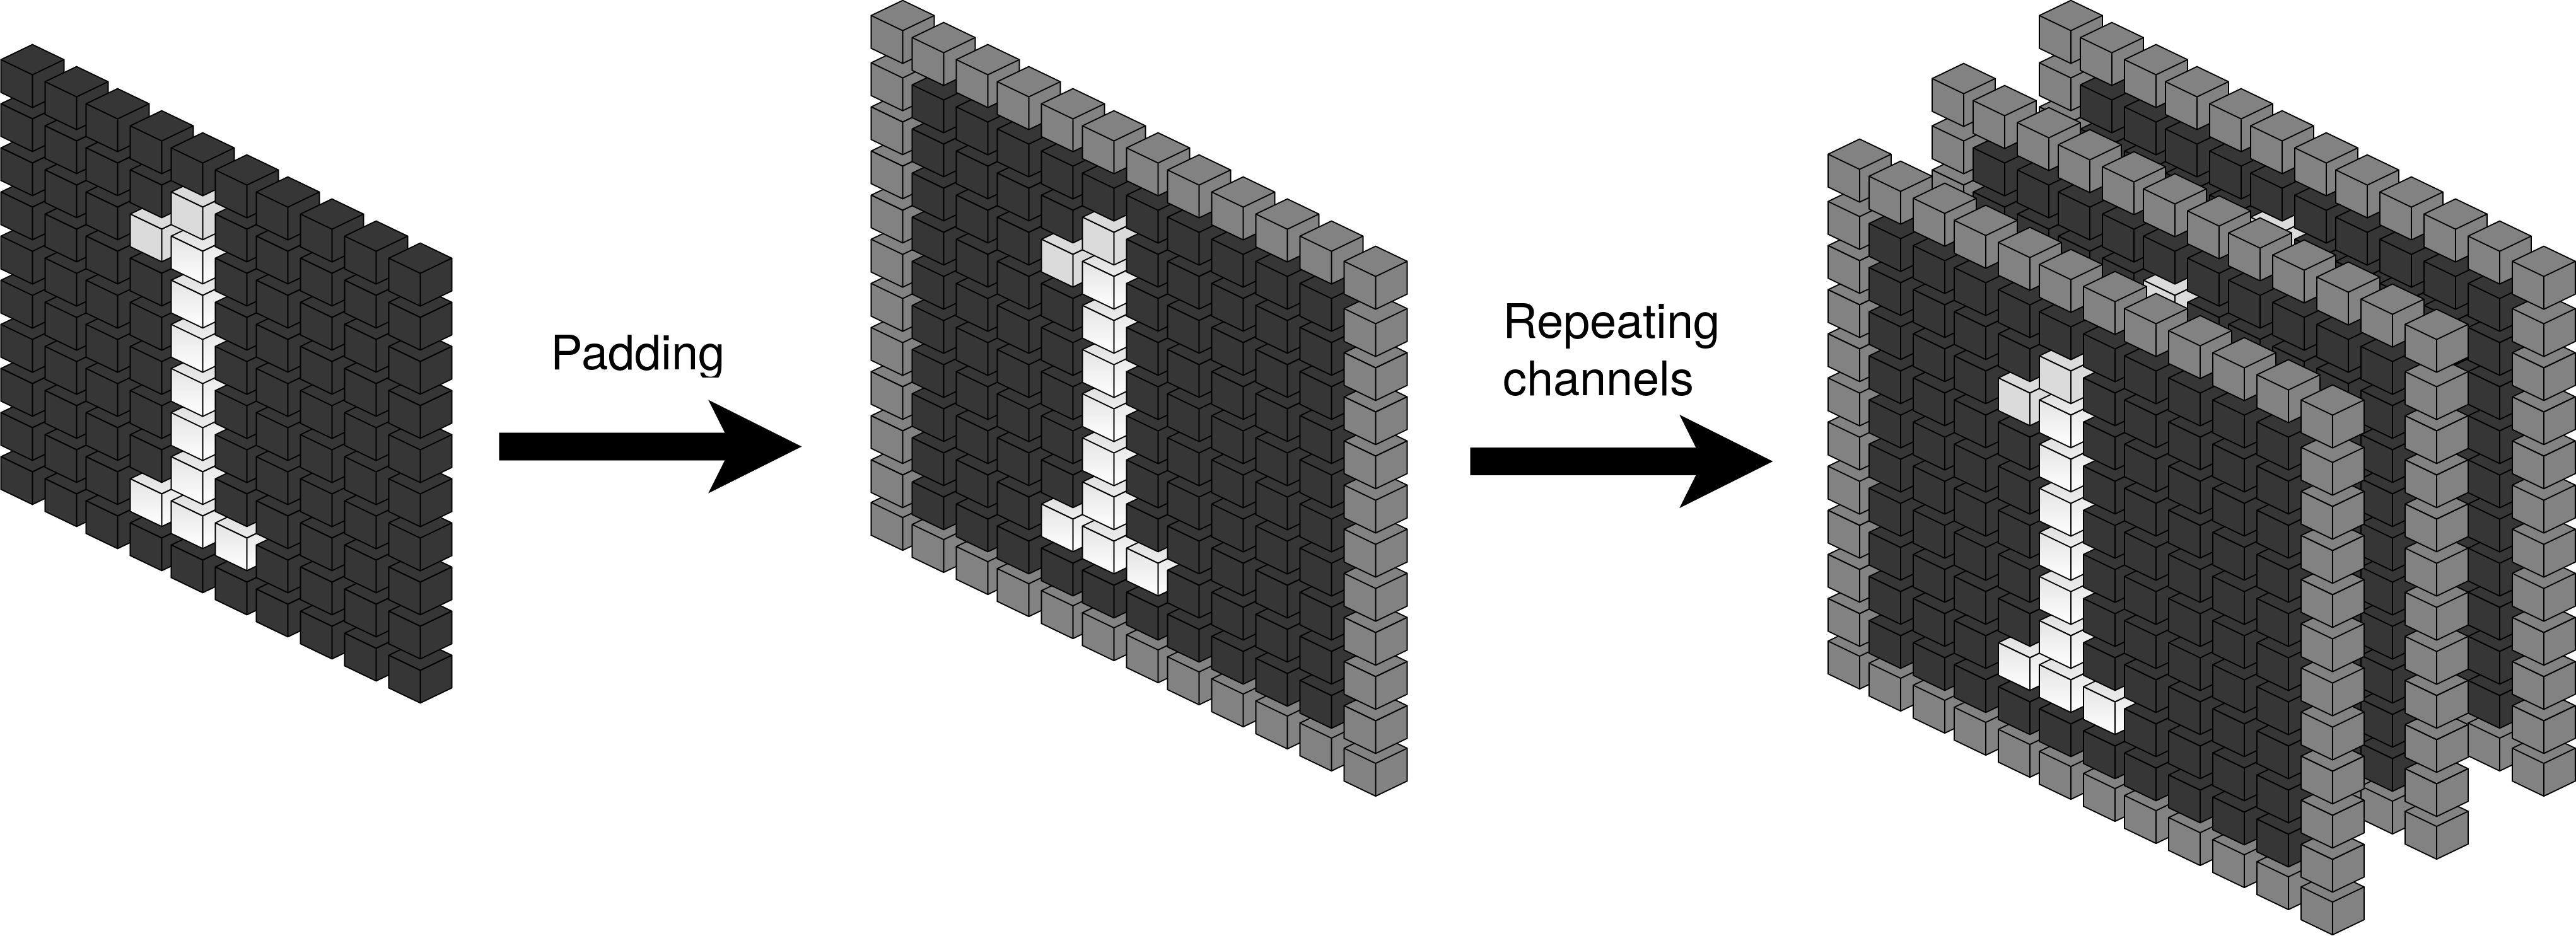
\includegraphics[width=\textwidth]{Chapters/Experiments/search_algo/figures/MNISTpadding+repeating.png}
    \caption{How MNIST is adapted to have same dimensions as cSVHN. Illustration use dimensions 12x12x3 while cSVHN and adapted MNIST use 32x32x3}
    \label{fig:MNISTpadding}
\end{figure}

\subsection{Tournament Search}
The tournament search uses a population size of 64, and as discussed, a winner-replaces-all replacement scheme between generations. Instead of using a accuracy threshold as in the previous experiments, the search terminates after 100 generations. A important feature of PathNet is the way learning is done. Since network back propagation occur during path fitness evaluation, the locked number of generations limit the amount of training that is allowed. In the original paper, fitness is set as the negative training error which is reached for each path after it have been trained for one training unit of 50 mini batches of size 16. This is an reasonable way of evaluating the fitness of a path when using a small tournament size, but as the tournament size have been increased tenfold for the algorithms with high selection pressure, fitness is calculated differently in these experiment. 

The problem of directly using the training error as fitness is that the error changes whenever weights along a path is updated. An extreme example can be used to present the underlying problem with this.

\begin{figure}[h]
    \centering
    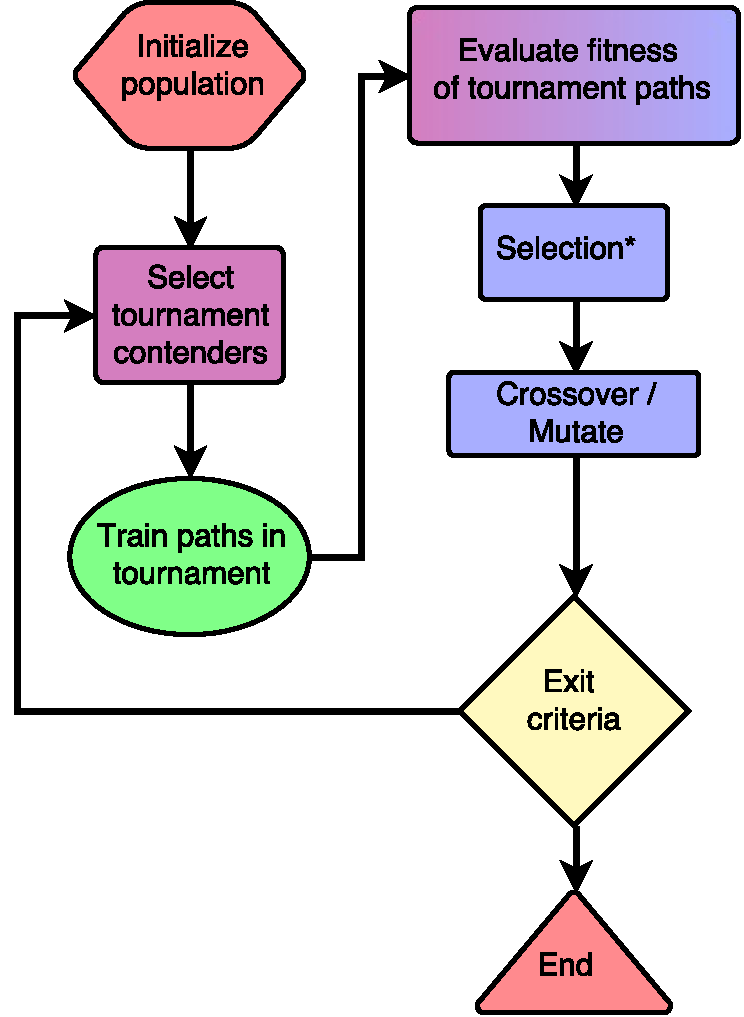
\includegraphics[width=0.5\textwidth]{Chapters/Experiments/search_algo/figures/TS_implementation.pdf}
    \caption{Flowchart of the tournament search implemented here. Compared to the flowchart of standard Tournament Search implementation in figure \ref{fig:algorithmflowcharts}, the difference is the extra step of training (green) before the fitness is evaluated. *The selection function always selects the tournament winner, except during algorithm 1c where the top two paths is selected.}
    \label{fig:ts_flowchart}
\end{figure}


Take a tournament selection of 25 genomes containing 24 identical paths and one different path with some module overlap to the others and which is evaluated first. One scenario could be that the first unique path is evaluated to a high fitness, when the next path evaluated, the weights in the modules which overlap between the two are updated. The evaluated fitness of the first path is now outdated, and for every subsequent path, this fitness might get worse and worse if the parameters in the overlapping modules move to an area of high error in the context of the first paths other modules. After all fitness evaluations, the first path now stands with a high fitness, which might be larger than that of all other paths in the tournament. Then all other paths in the tournament is replaced with the winning path even if its actual fitness might have become significantly reduced during the evaluation step. Due to this, the fitness of paths in a tournament is calculated in a separate step for these experiments as seen in figure \ref{fig:ts_flowchart}. After a subset of the population is selected for a tournament, all paths in that tournament are trained for one training unit. When training is completed, each path is evaluated by using a new subset of the training data for validation. This way, the order in which paths are validated does not affect the fitness score, which is the classification accuracy reached during the validation step. The order of paths still affect the the training but the fitness used for selecting a tournament winner is the "true"\footnote{Fitness is still calculated on the basis of the training data-set, which means it might become overly optimistic over time. Overfitting during training is discussed in the context of another experiment} fitness score.

The same reason influence the final step of the tournament search. When the limit of a hundred generations is reached, all paths in the population is evaluated again. Since the true fitness of a path might change from one generation to the next, only the paths participating in the final tournament has its true fitness score as part of the selection of the optimal path. As with the evaluation step, the final fitness of a path is the reached classification accuracy of one training unit (50 mini-batches of 16 samples). Using an actual validation set for this step might yield better, or at least more accurate, fitnesses to use as a basis for path-selection, but that would significantly increase the run-time of an already time intensive experiment. 

\section{Results}\label{Search-results}
Due to the experimentation being time-consuming, each algorithm were run 10 times and logs were saved after each experimental run of each algorithm. The following plots have been separated in three groups based on subject: paths, search and training. 

\subsection{Paths}
\begin{figure}[p!]%[h]
    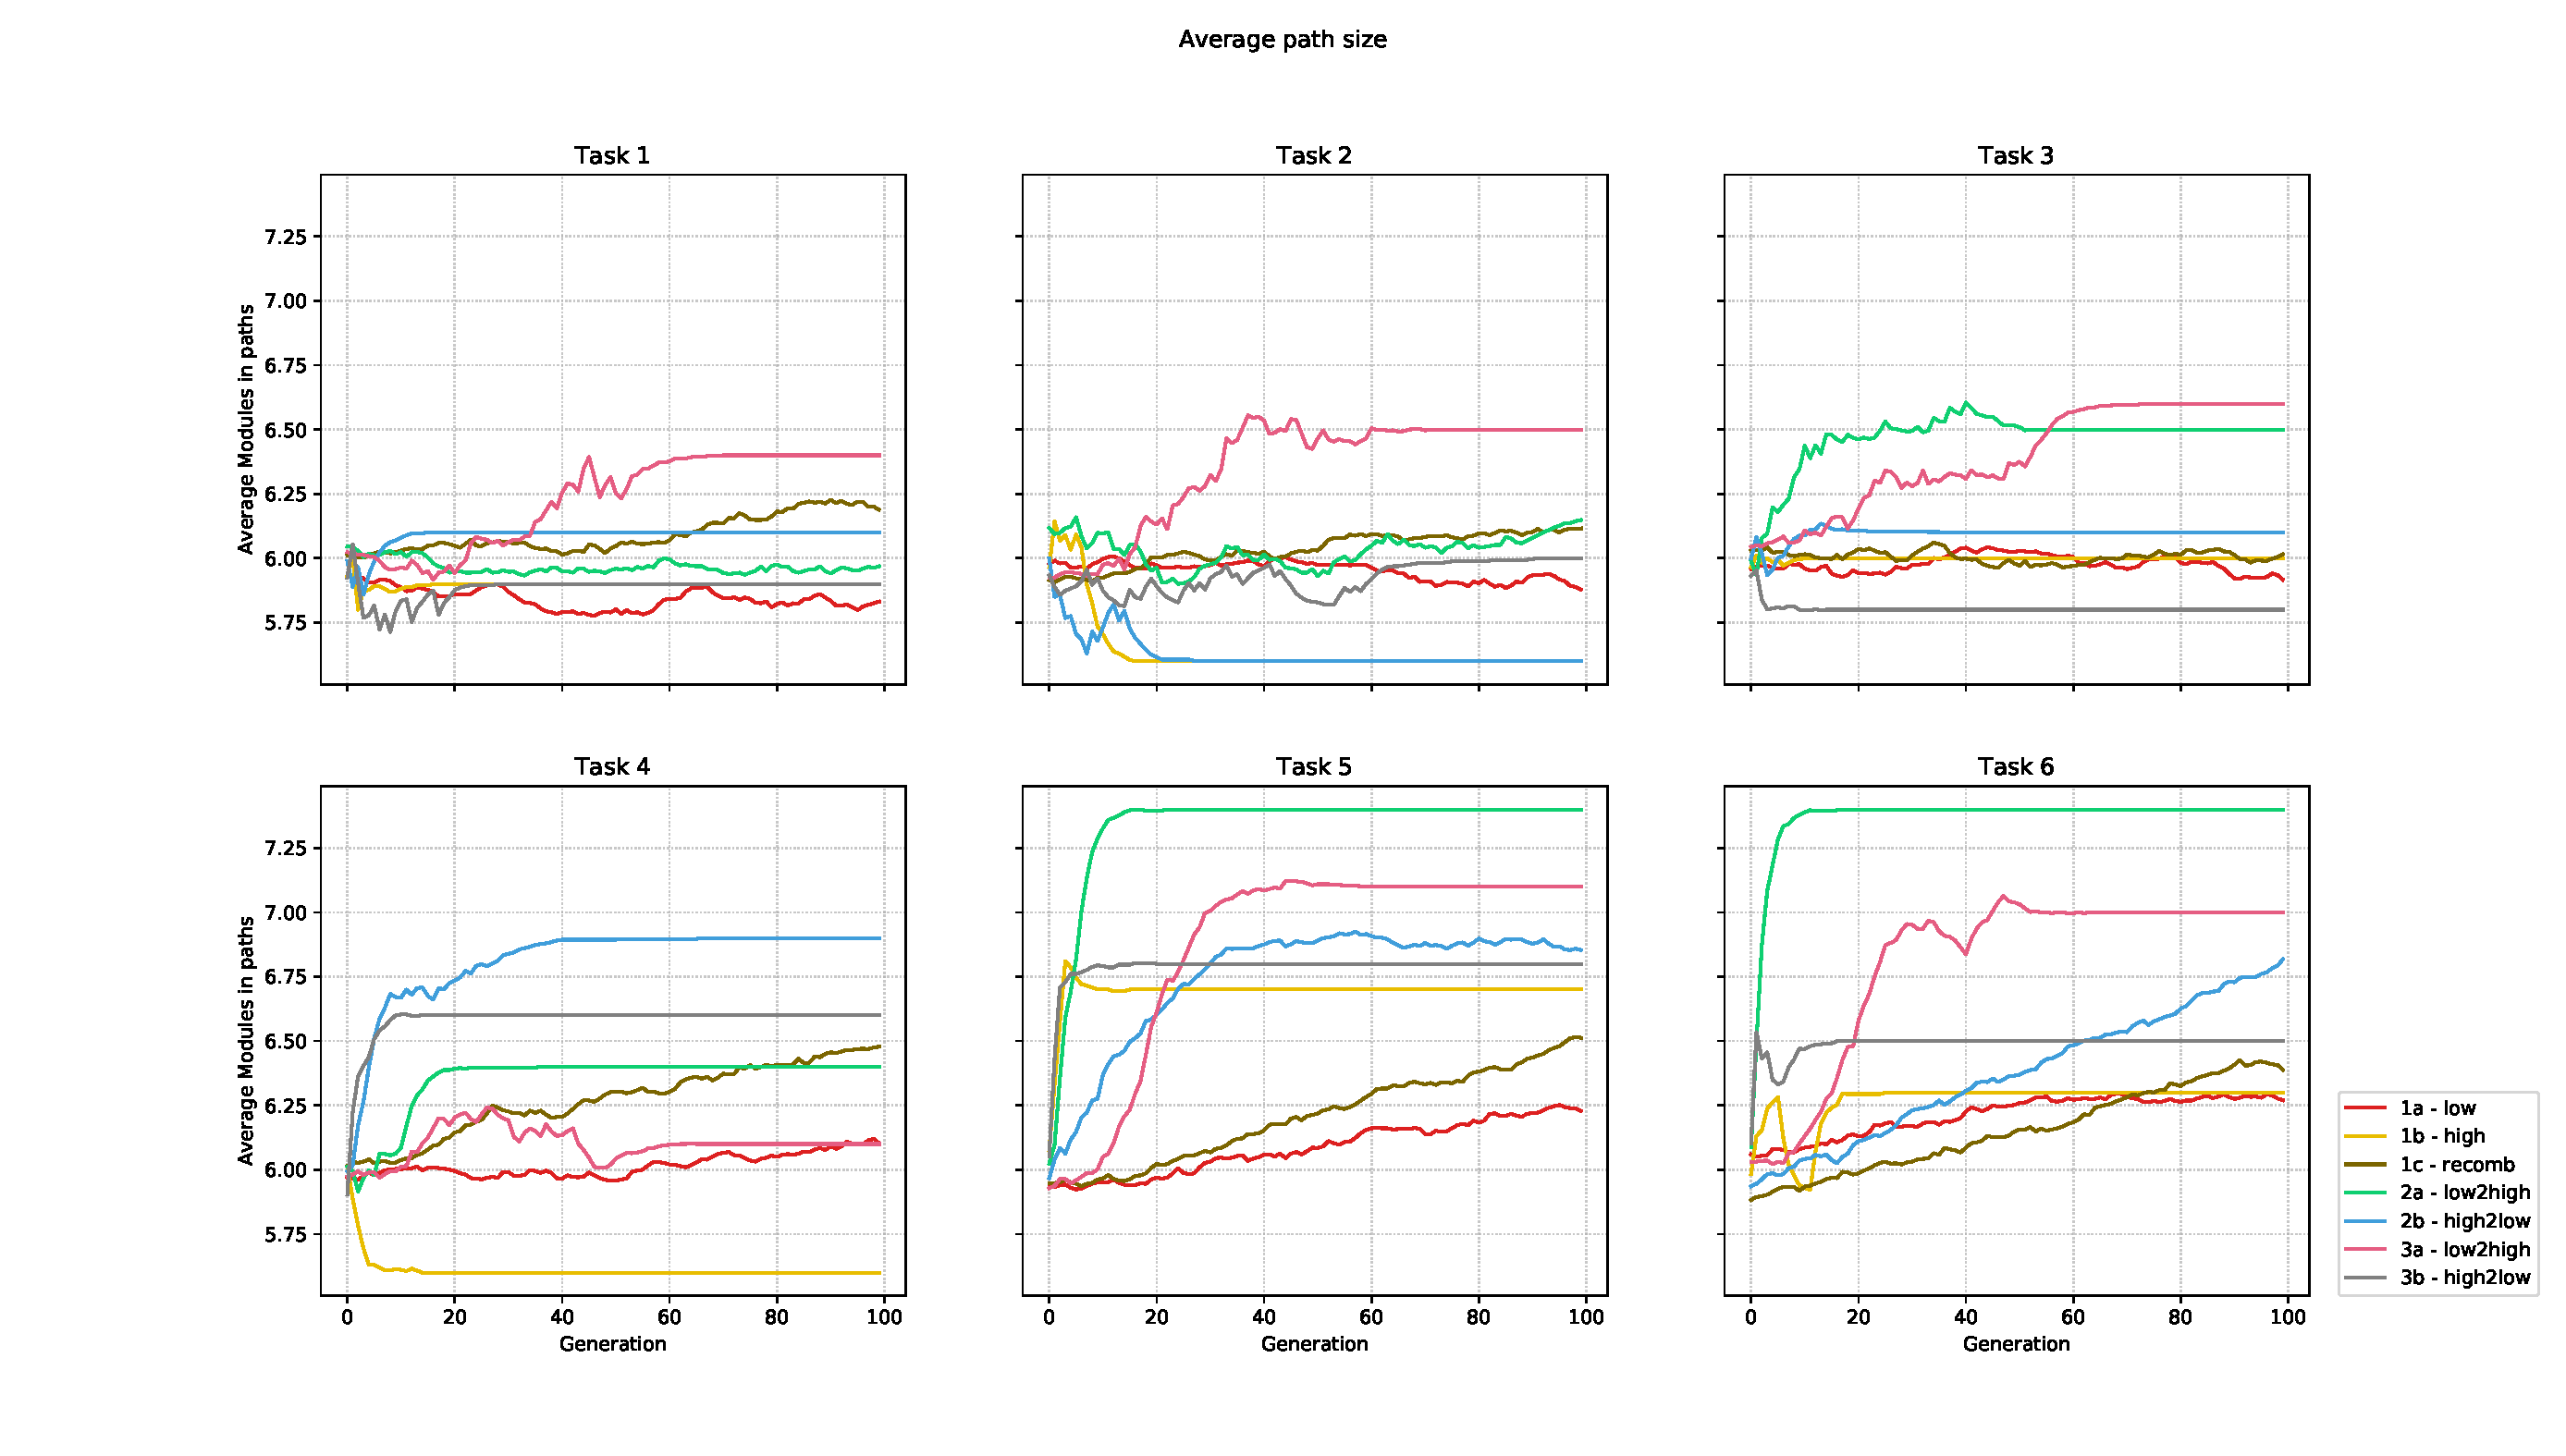
\includegraphics[width=1.2\textwidth,center]{Chapters/Experiments/search_algo/figures/Average_path_size.pdf}
    \caption{Change in average path size for each tournament scheme plotted for each task.}
    \label{fig:search.avg_path_size}
\end{figure}

Figure \ref{fig:search.avg_path_size} visualize the average path size within the average population for all generations. Each subplot is for one task and the search for that tasks optimal path. As each path contains between three and nine modules, the average path size is six and this is reflected in the plots where this is the initial value for the first generations. Each search starts with a randomly initialized population of paths. Note the span of sizes plotted reach from around 5.5 to around 7.5, which indicates the average initialized size of 6 does not contain enough capacity as more often than not, the searches converges towards larger path sizes, especially for the later three tasks based on the cSVHN set. 

A feature of this plot is the steep jump and quick convergence to a size for the searches with high selection pressure for the early generations. Since mutation only causes the index of a module to change by a value between -2 and 2, the size of a path can not change during mutation\footnote{A path can not include the same module multiple times. If a module is mutated to overlap an existing one, it is removed. This causes the path to contain fewer modules, so mutated modules are added back in until original path size is reached.}. This means when algorithms with high selection pressure converges to a size early in the search, the size of paths can never change. For searches with low selection pressure (algorithm 1a, 1c, 2a for the earlier tasks and 2b for the later tasks), the generation limit of 100 is to low to let them reach an optimal size. 

\begin{figure}[p!]%[h]
    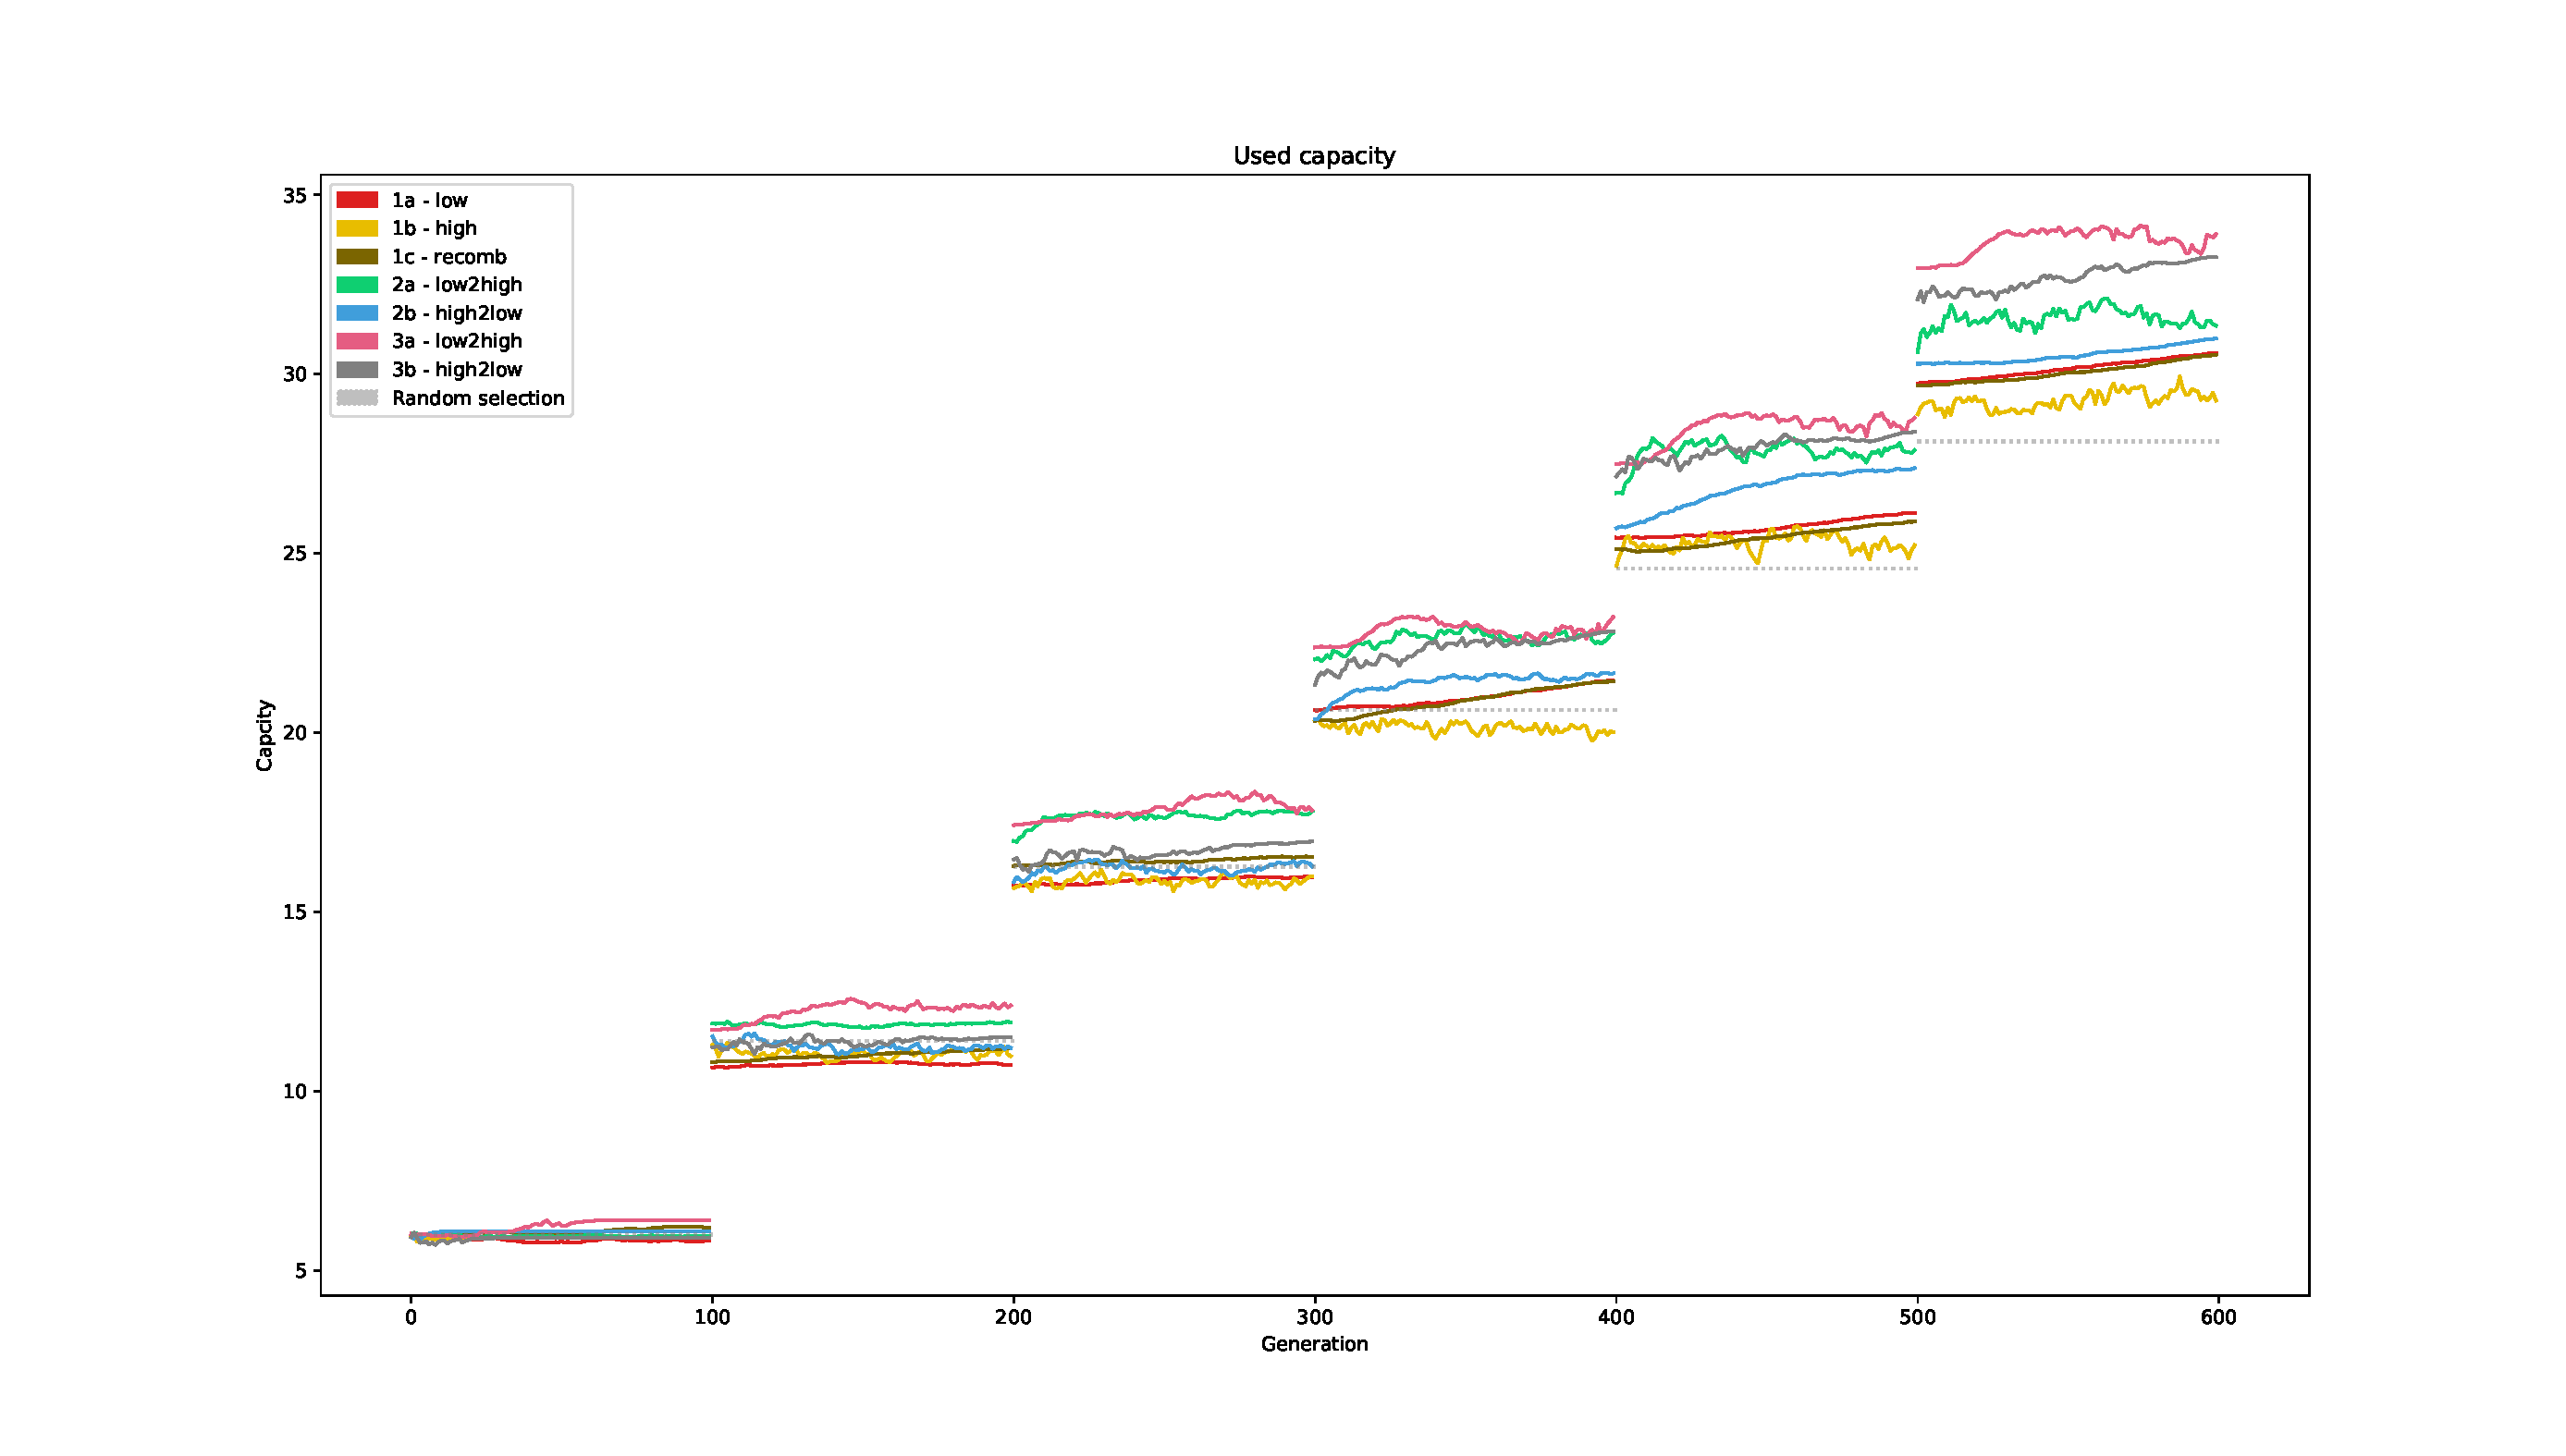
\includegraphics[width=1.2\textwidth,center]{Chapters/Experiments/search_algo/figures/Capacity_pr_generation.pdf}
    \caption{The average number of used modules during the multi-task learning sequence. Each jump is caused by the saving of an optimal path and then starting a new search for a new task. }
    \label{fig:search.capacity}
\end{figure}

In figure \ref{fig:search.capacity} we can see some of the influence of path size in the average cumulative amount of capacity used during all generations. As with plot \ref{fig:search.avg_path_size}, the curves starts at capacity 6 and for the same reason. 

For task 4 the capacity usage have separated for the three algorithm groups. All algorithms with static tournament size use less modules in the total PathNet than the other algorithms, and algorithms with changing tournament size between tasks use less than group three. Note that all algorithms has a higher capacity usage than the dotted gray line which marks the amount of module reuse that would have been reached for 6 tasks if all paths had a random module selection\footnote{These values are reached by a Monte Carlo approach where \(10^{6}\) sequences of 6 random paths were selected in the same sized PathNet and the capacity used averaged.}.

\begin{figure}[p!]%[h]
    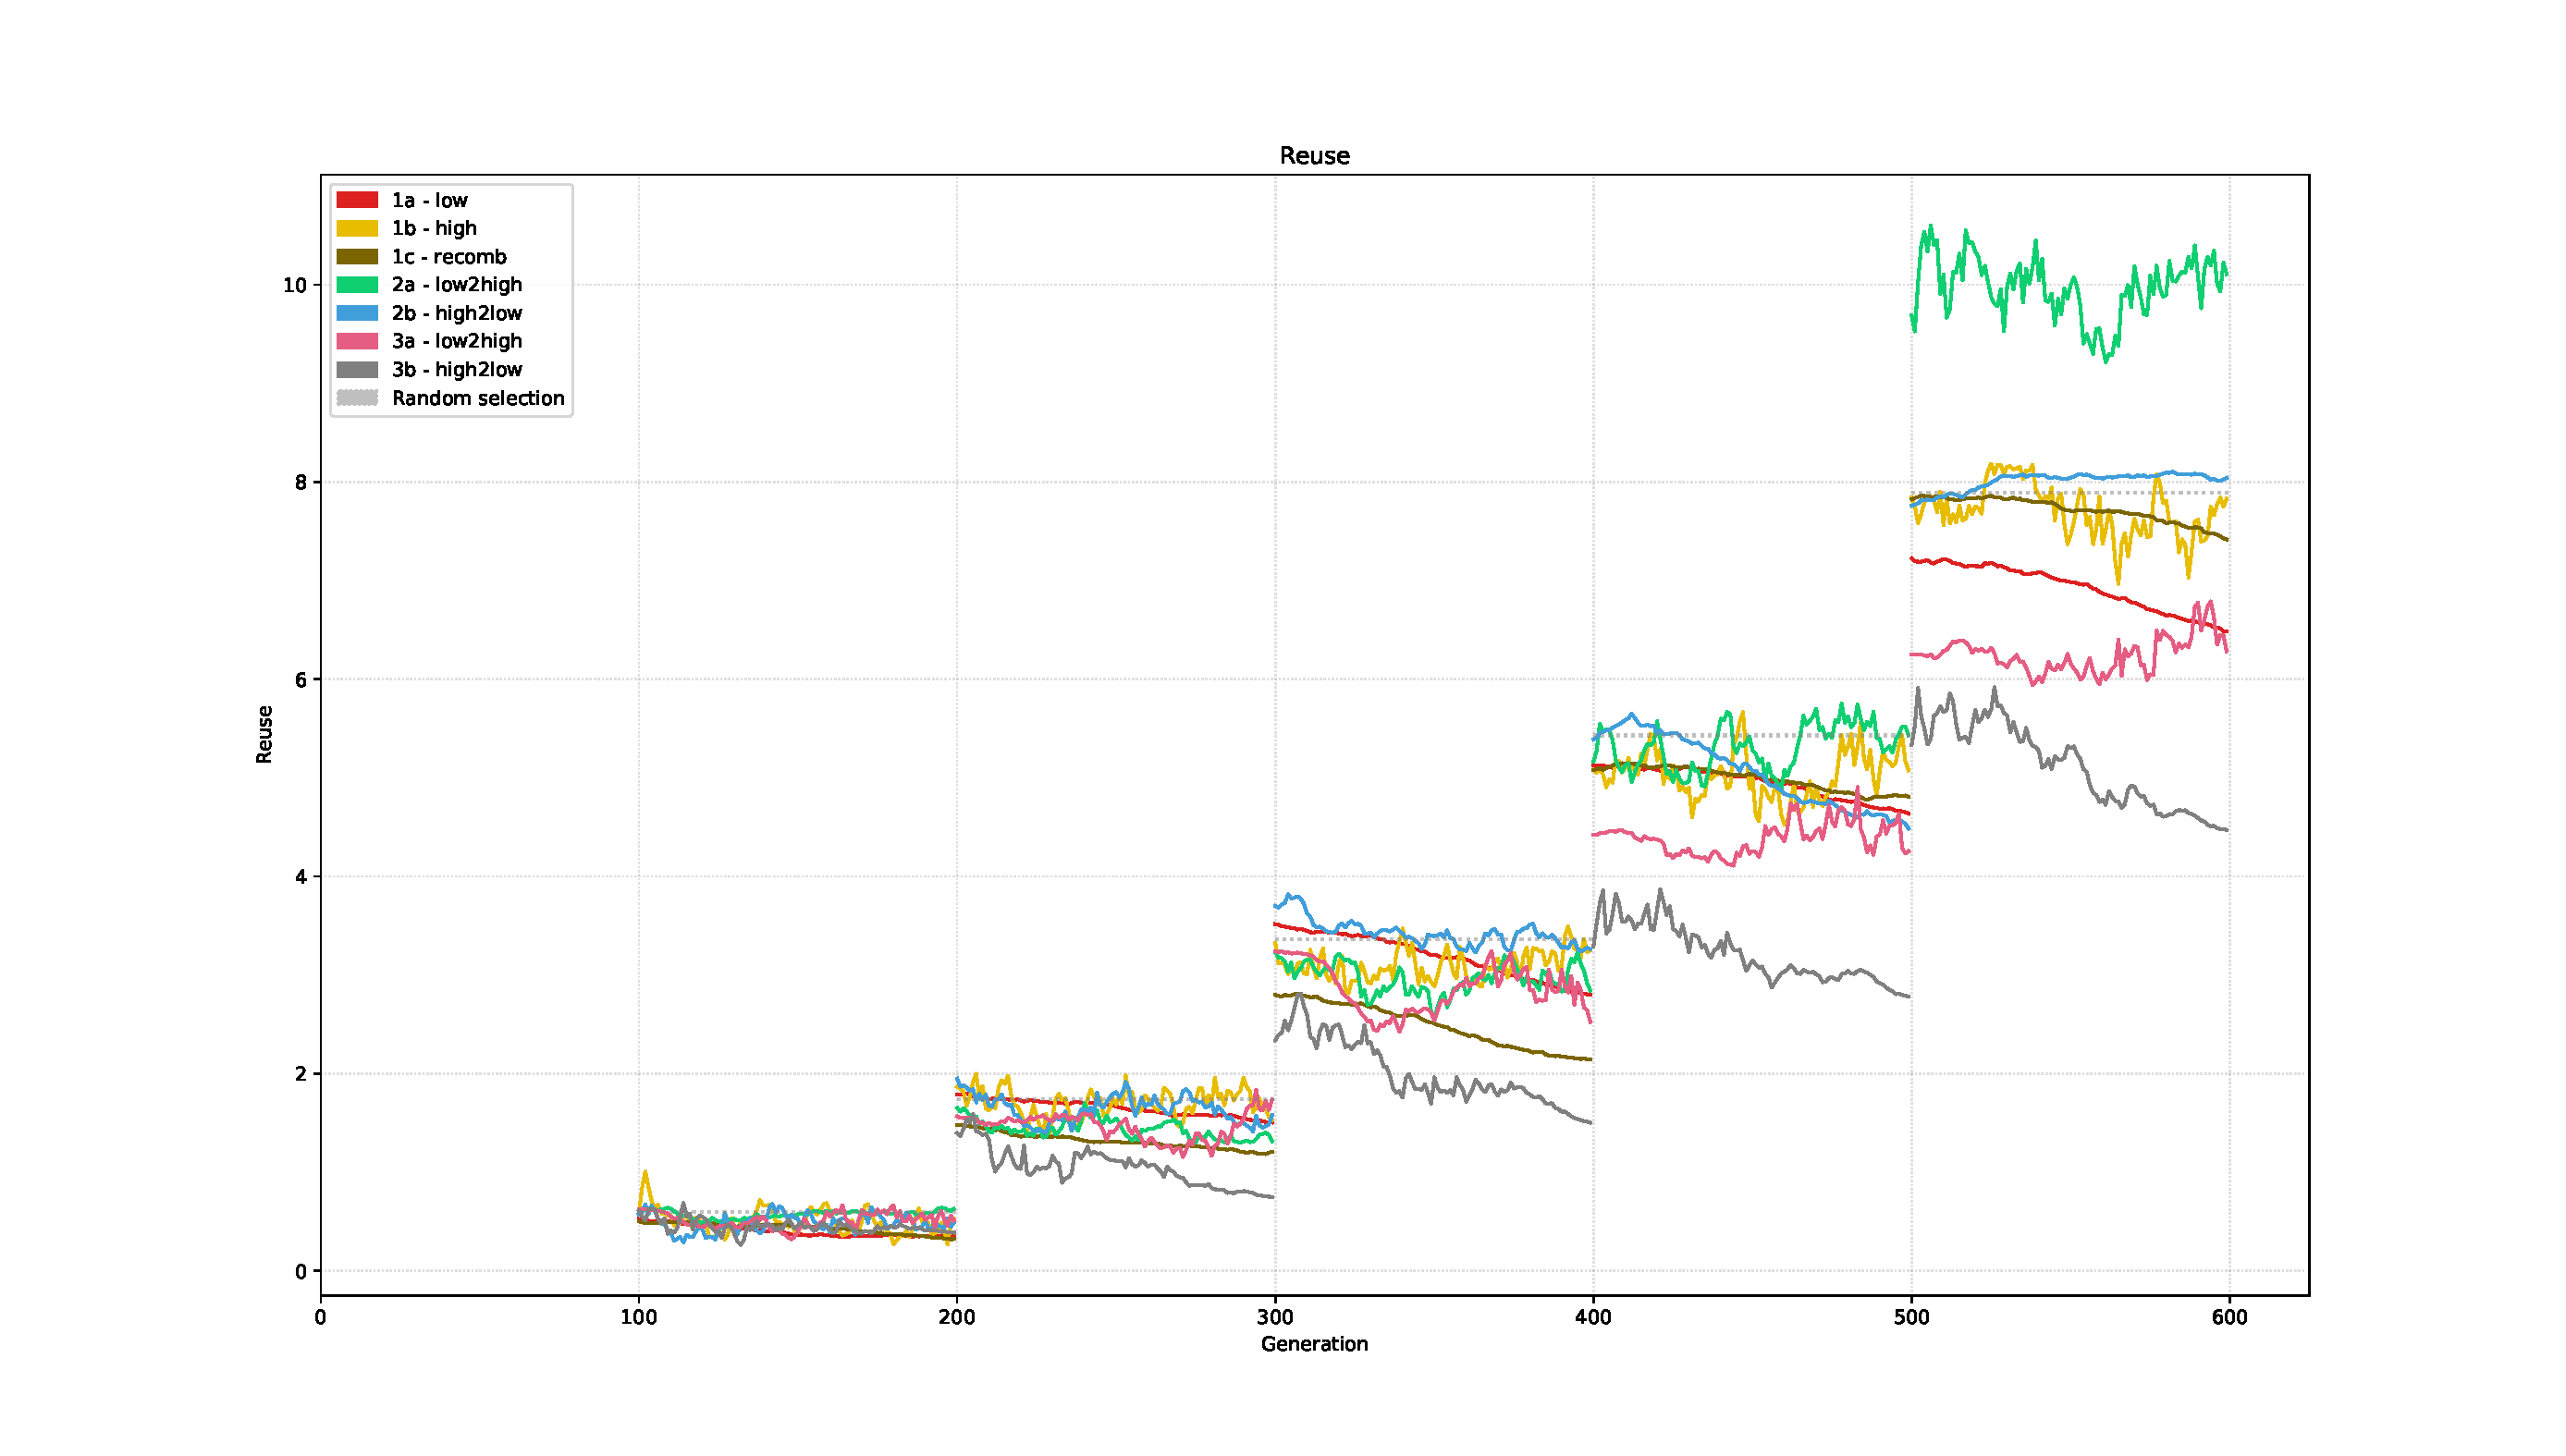
\includegraphics[width=1.2\textwidth,center]{Chapters/Experiments/search_algo/figures/Module_reuse_pr_generation.pdf}
    \caption{The average module reuse during the multi-task learning sequence. Each jump is caused by the saving of an optimal path, and the next task having more locked modules to reuse. The first 100 generations does not have any previously learned knowledge to reuse.}
    \label{fig:search.reuse}
\end{figure}

The similar plot \ref{fig:search.reuse} show how the average amount of module reuse change during the generations. As with plot \ref{fig:search.capacity}, the dotted grey line represents the amount of module reuse in a random selection of modules\footnote{These values are reached by a Monte Carlo approach similar to plot \ref{fig:search.capacity}.} instead of search. Between the two last tasks we see a large jump in module reuse for algorithm 2a compared to the rest. The dynamic tournament size algorithms 3a and 3b has the least reuse for task 4 and 3b seem to lower its reuse significantly from the initial value during each search. 

When visualizing search features for the different algorithms that stem from different generations during each search, the algorithms using a high tournament size have curves undergoing rapid changes and algorithms using low tournament sizes have curves with more gradual changes. Plot \ref{fig:search.reuse} is no different, which can make it hard to tell if there is an increase or decrease in reuse for algorithms 1b and 2a during the last 600 generations. To validate the results, one-way ANOVA test have been run on the mean number of reuse for each algorithm after the 6 tasks are trained (see \ref{search-discussion:dynamicselectionpressure} for test results).

\subsection{Population Diversity}
\ref{fig:search.hamming_diversity} visualizes the average population diversity for each algorithm for each task calculated with the pair-wise Hamming distance metric. As this metric is dependent on the size of population as well as the number of genes in a genotype, the value at one point in the generation is not depictive of anything, but instead, the overall trend of the measure indicates at what rate the algorithm converges. 

\begin{figure}[p!]%[h]
    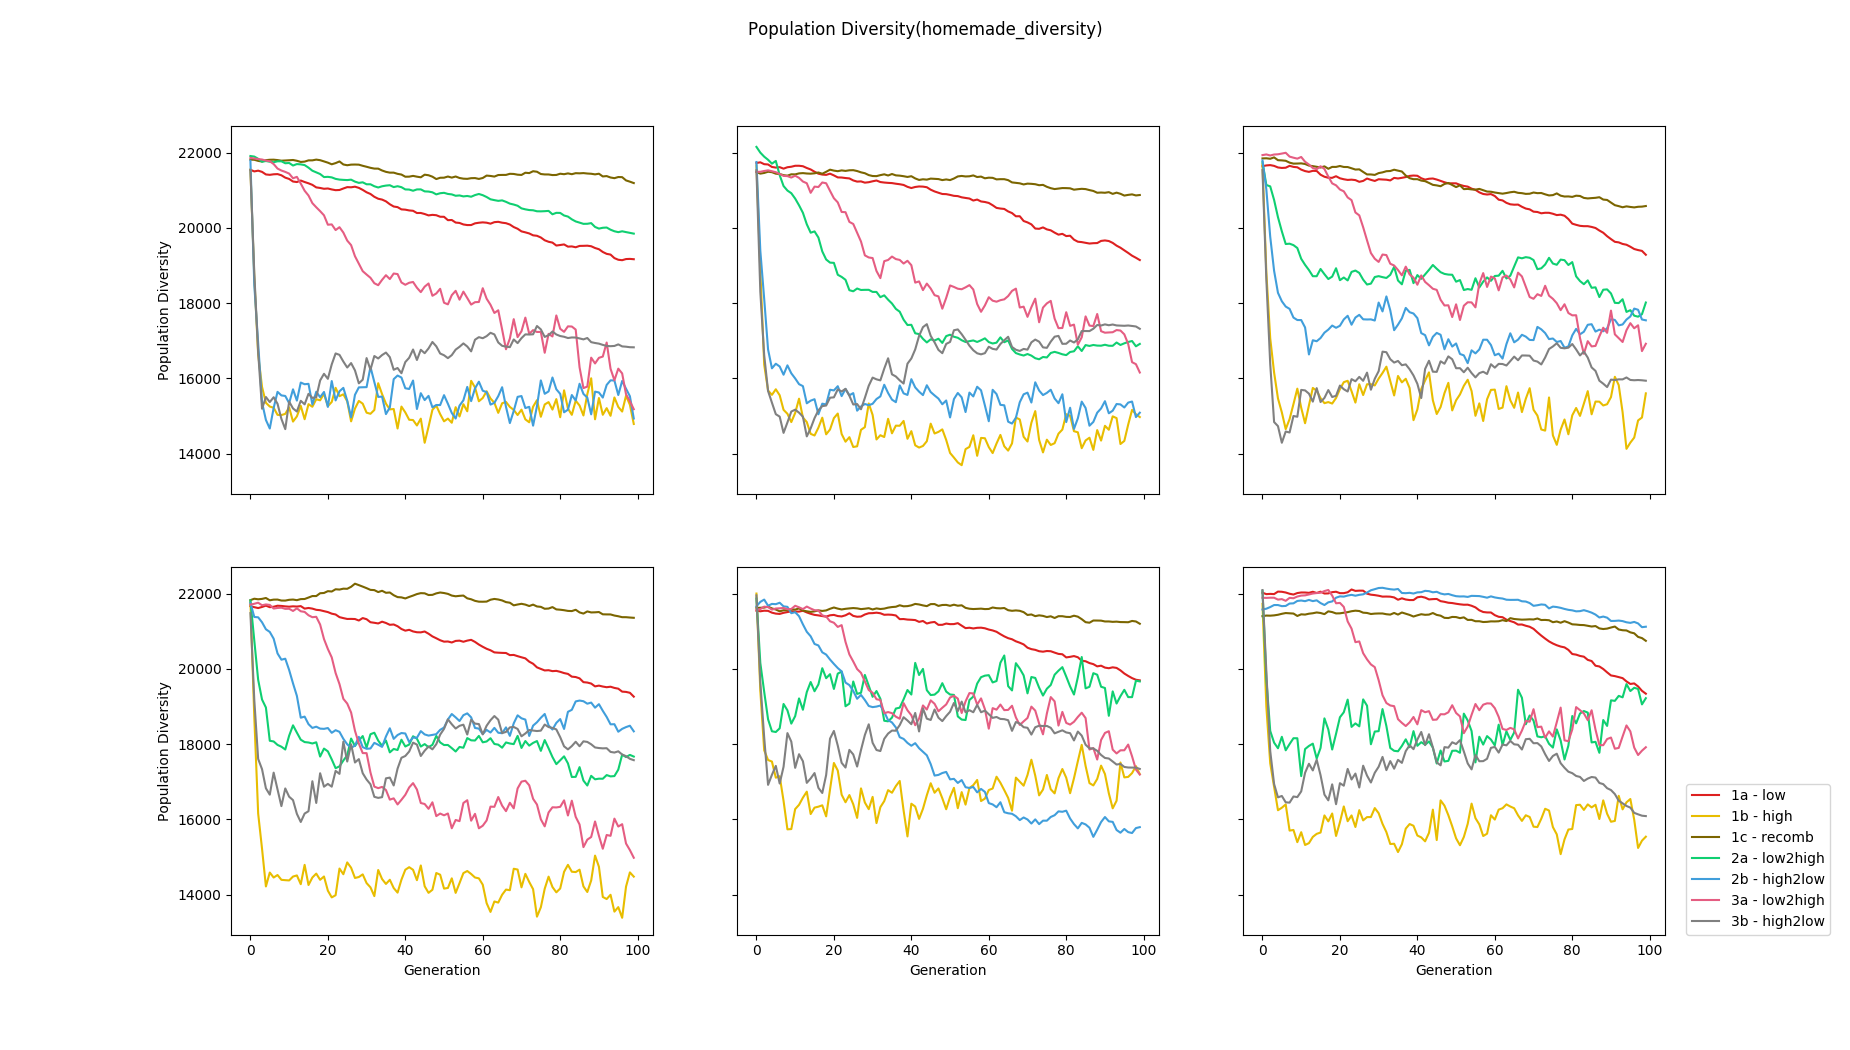
\includegraphics[width=1.2\textwidth,center]{Chapters/Experiments/search_algo/figures/Average_population_diversity_reduced_hamming.png}
    \caption{The average pairwise Hamming distance within each generation is used as a measure for population diversity. Each subplot (in order left to right) is each task in trained order.}
    \label{fig:search.hamming_diversity}
\end{figure}

As with plot \ref{fig:search.avg_path_size}, high selection pressures lead to rapid changes in diversity. This is because the searches with high selection pressure have a high tournament size compared with the population size. When a generation is over and  the tournament winner replace all losers, the population makes a large shift in diversity unless most of the tournament participants have a similar genome. At that point, the probability that the population have converged is quite large. 

\begin{figure}[p!]%[h]
    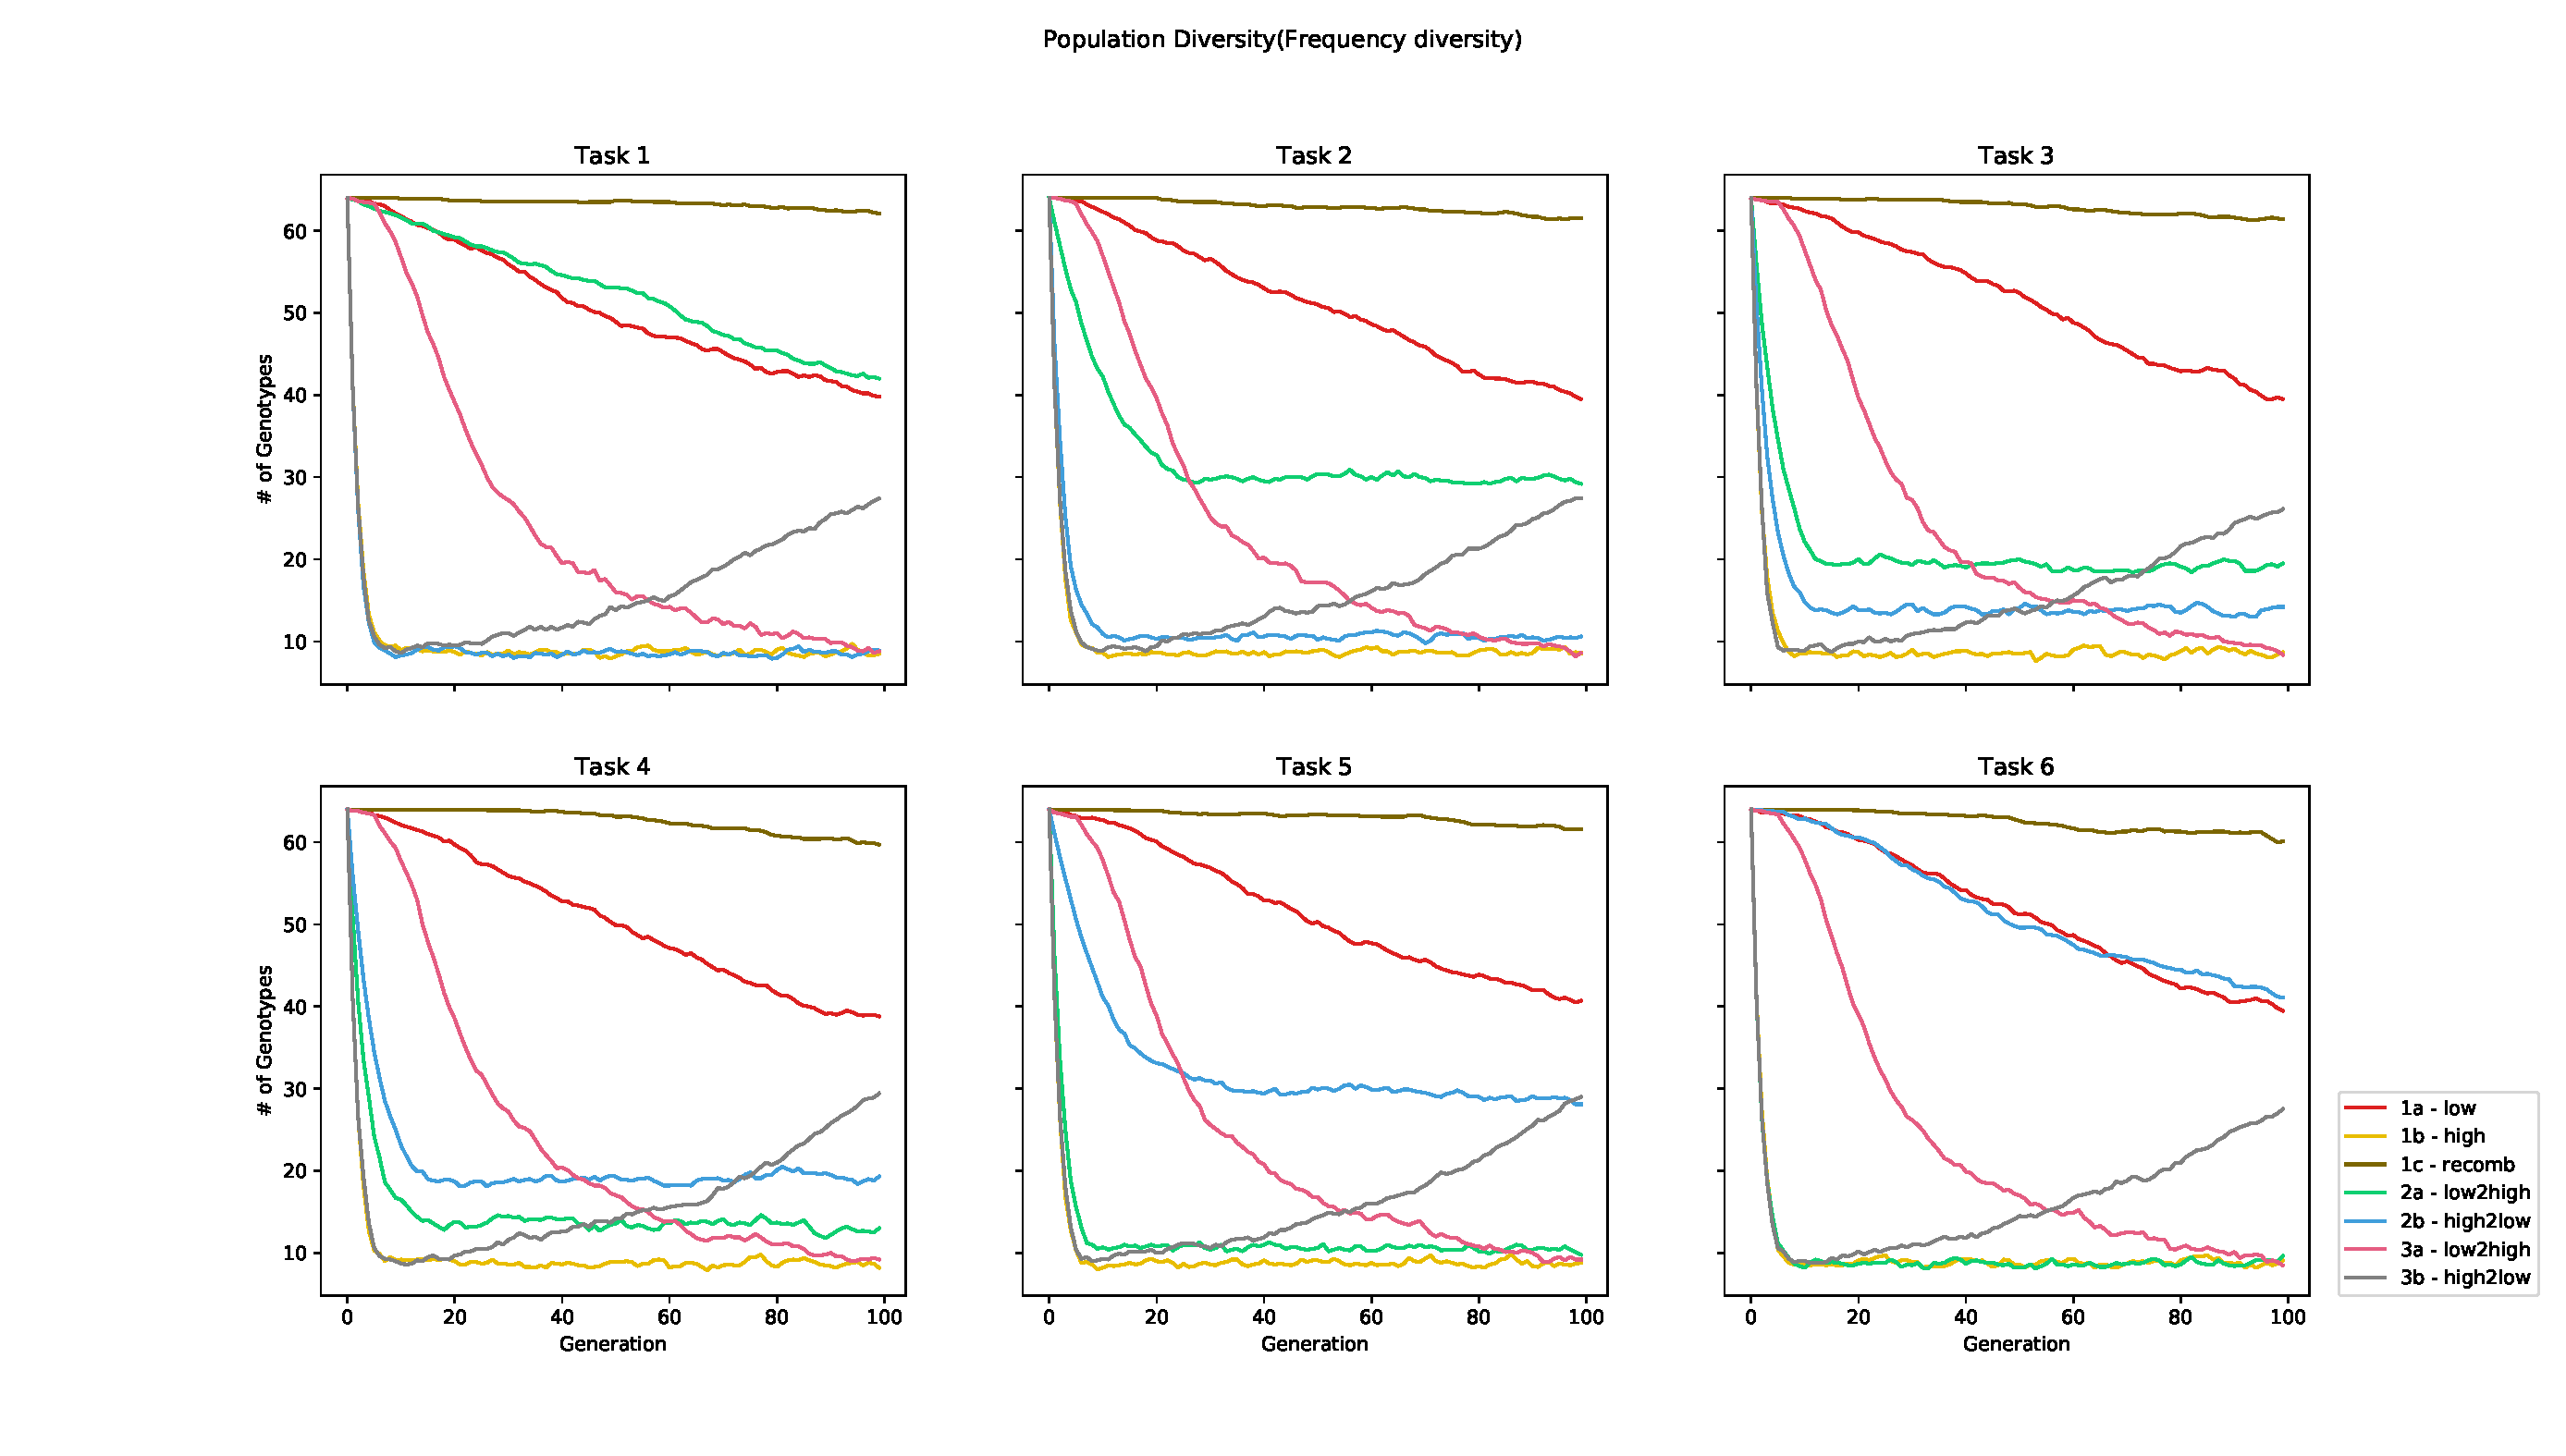
\includegraphics[width=1.2\textwidth,center]{Chapters/Experiments/search_algo/figures/frequency_diversity_unique_path_count.pdf}
    \caption{The number of unique paths within a population. Plotted for every task and every algorithm.}
    \label{fig:search.frequency_diversity_unique}
\end{figure}

The Hamming distance between two binary genomes gives what is essentially the edit distance and not a measure of the fundamental difference between the genomes. This means the Hamming metric is accurate and quite descriptive when looking at one gene at a time, but for larger genomes can be somewhat misleading in some circumstances. Take for instance, a population consisting of three even groups of three types of genomes. If one group is replaced with genomes from the two other groups such that the population consists of two equal parts of each genome, the diversity of the whole population have gone down\footnote{This is fairly obvious since we in this scenario is left with only two types of genomes, while we started with three}, but the pair-wise Hamming distance might have gone up. Because of this, it is hard to tell if the constantly high diversity levels is caused by using pair-wise Hamming distance as metric, or for instance high mutation probabilities. This effect becomes clear when comparing plot \ref{fig:search.hamming_diversity} with plot \ref{fig:search.frequency_diversity_unique}. This plot visualizes the amount of unique paths in a population and has therefore some problems as a diversity metric that Hamming distance does not. A mutated genome would be considered to be a similar genotype to its original state, and a pair-wise Hamming distance would reflect this by only counting the small genome change between these two. On the other hand, a unique genotype frequency metric would count these two genotypes as completely different. However, together these plots provides a better picture of the diversity than either does alone. \textit{Editnote: will change in new results}
% New results

\subsection{Training}
\begin{figure}[p!]%[h]
    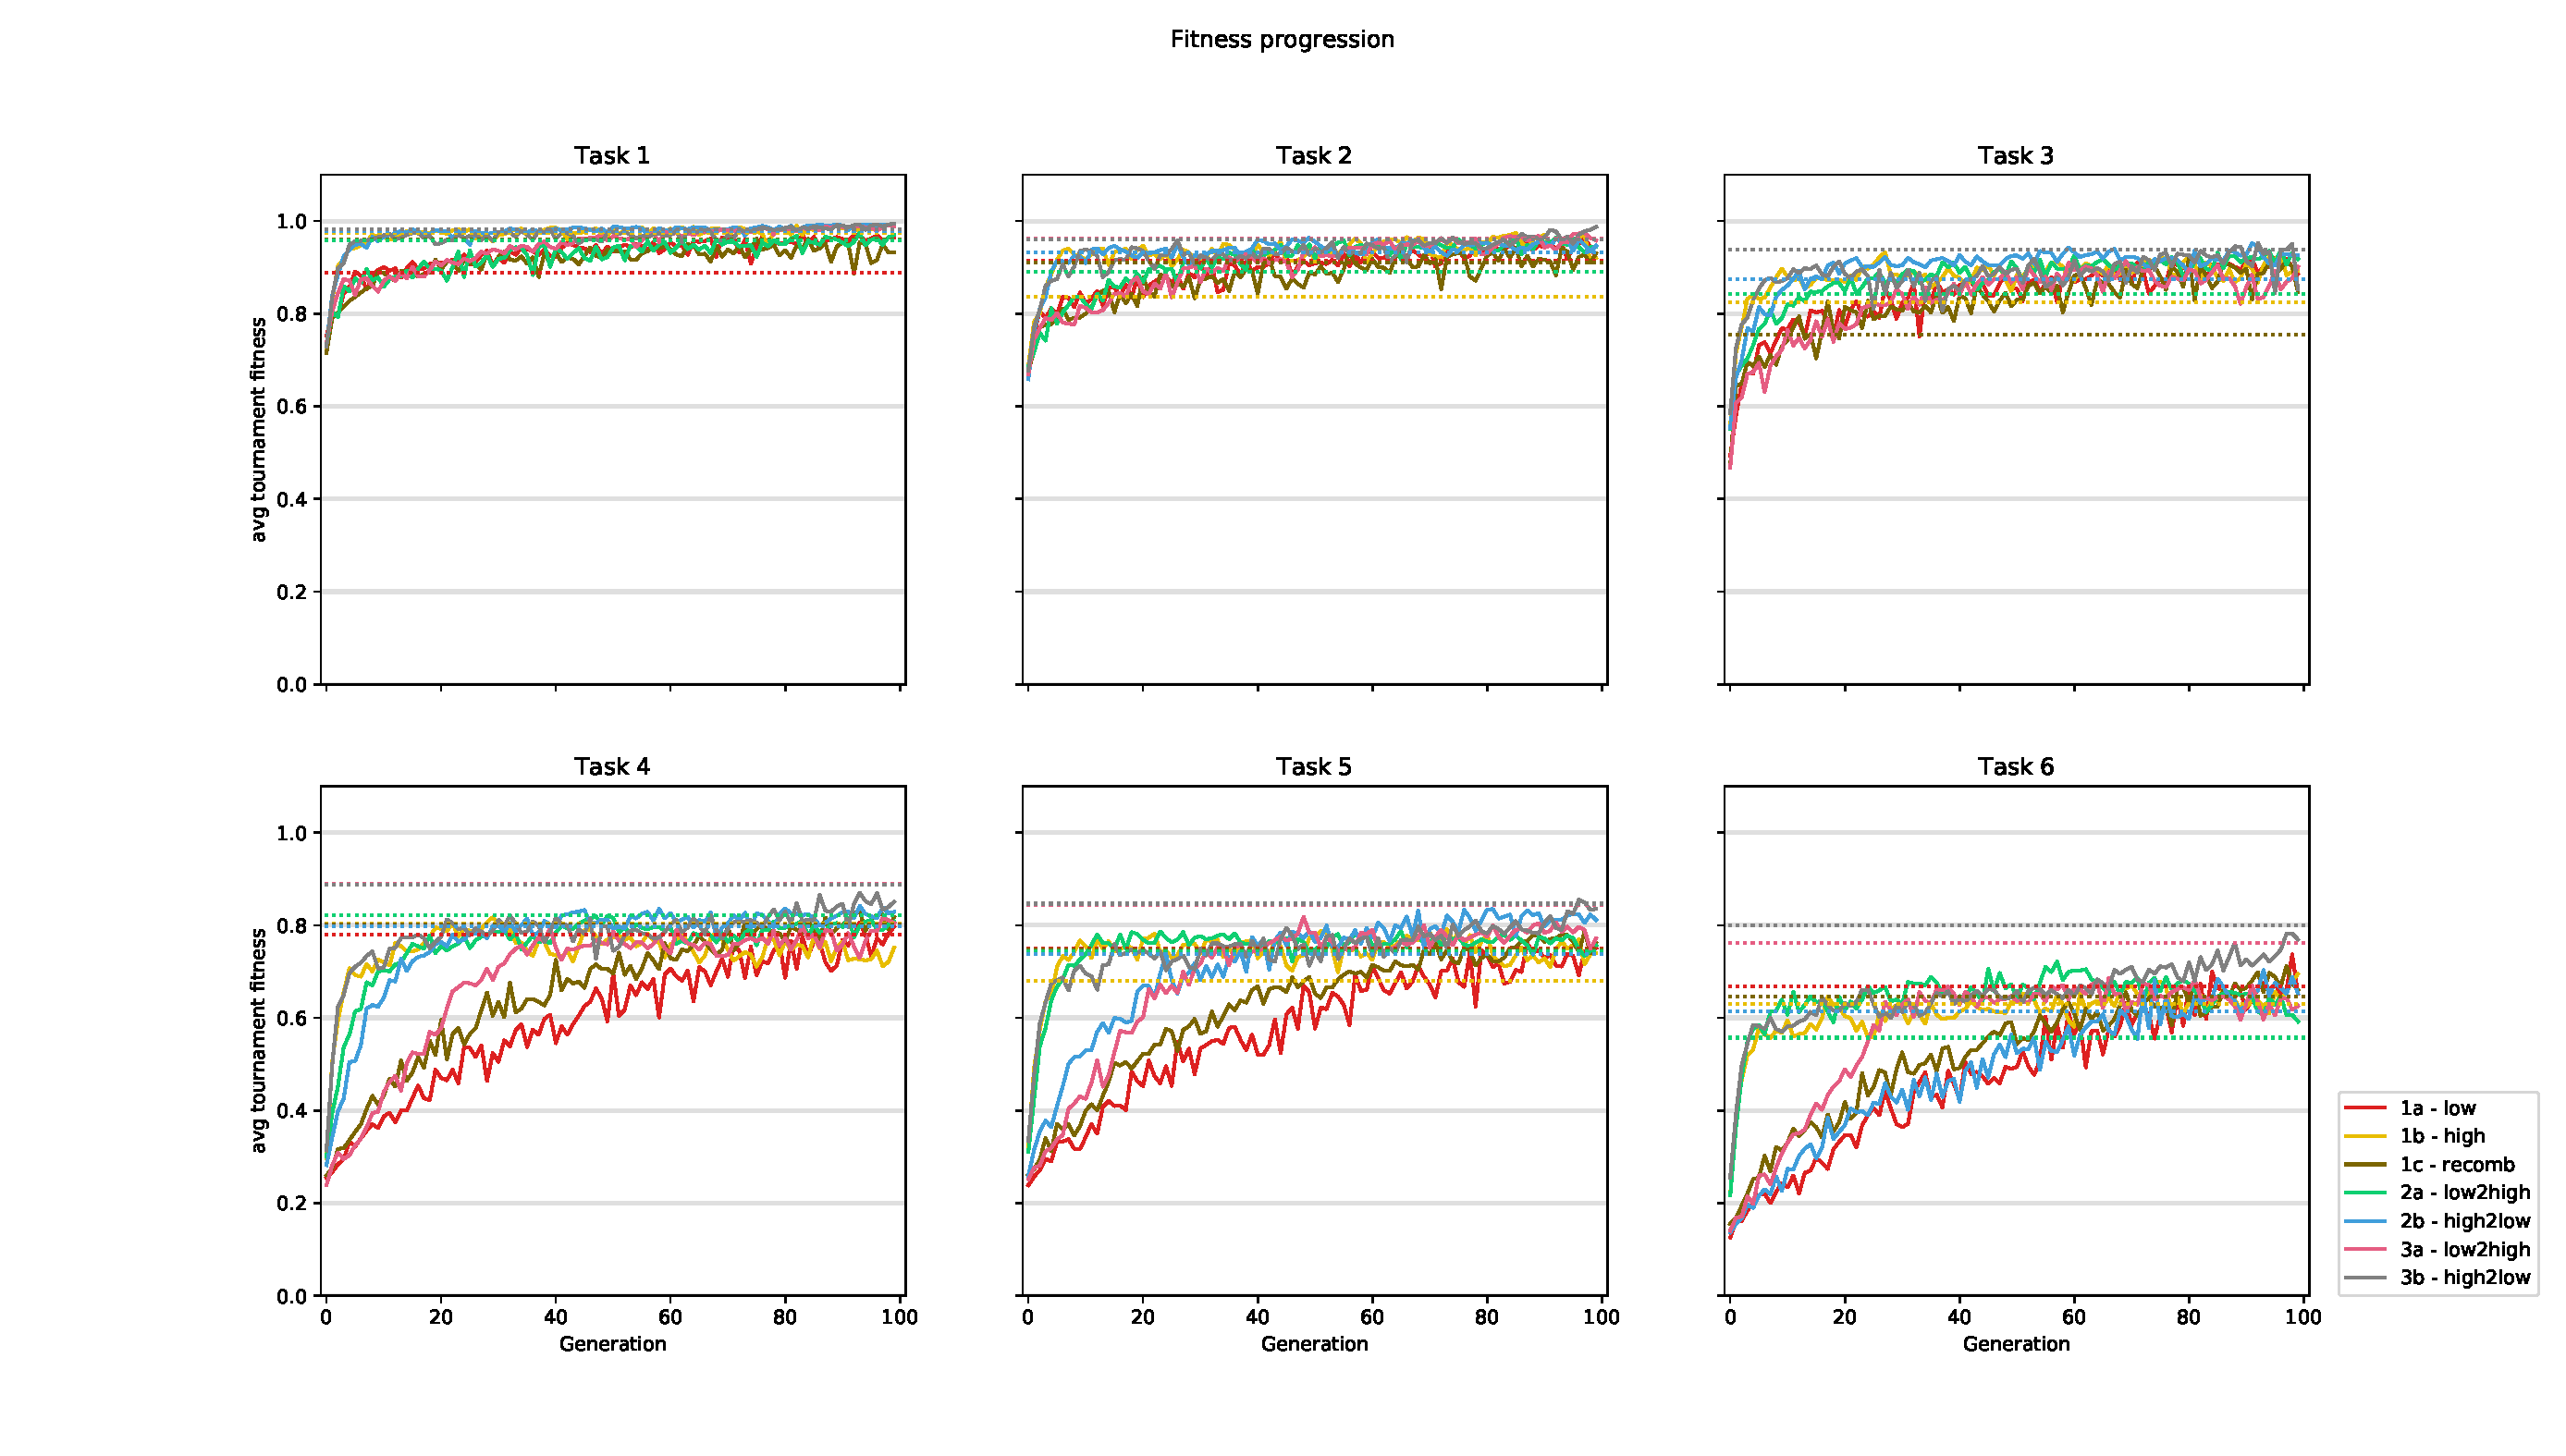
\includegraphics[width=1.2\textwidth,center]{Chapters/Experiments/search_algo/figures/Training_accuracy.pdf}
    \caption{Average training accuracy during search. The dotted lines is the average achieved validation accuracy for that task and that algorithm.}
    \label{fig:search.accuracy}
\end{figure}
As the training of each path is done during and controlled by the search, how the average training accuracy develops gives an indication of how quickly the algorithms are able to influence the overall PathNet to learn a task. As discussed previously, the act of training one tournament of genomes effect the previously evaluated fitness values. Because of this, the populations average fitness values would be a highly misleading metric to use and therefore what is plotted here is the average fitness score achieved within a each generations tournament. Also plotted is the mean validation accuracy reached for each algorithm. This validation score is only calculated after an optimal path have been found for each task, and can therefore not be viewed as a function of generation number. 

\begin{figure}[p!]%[h]
    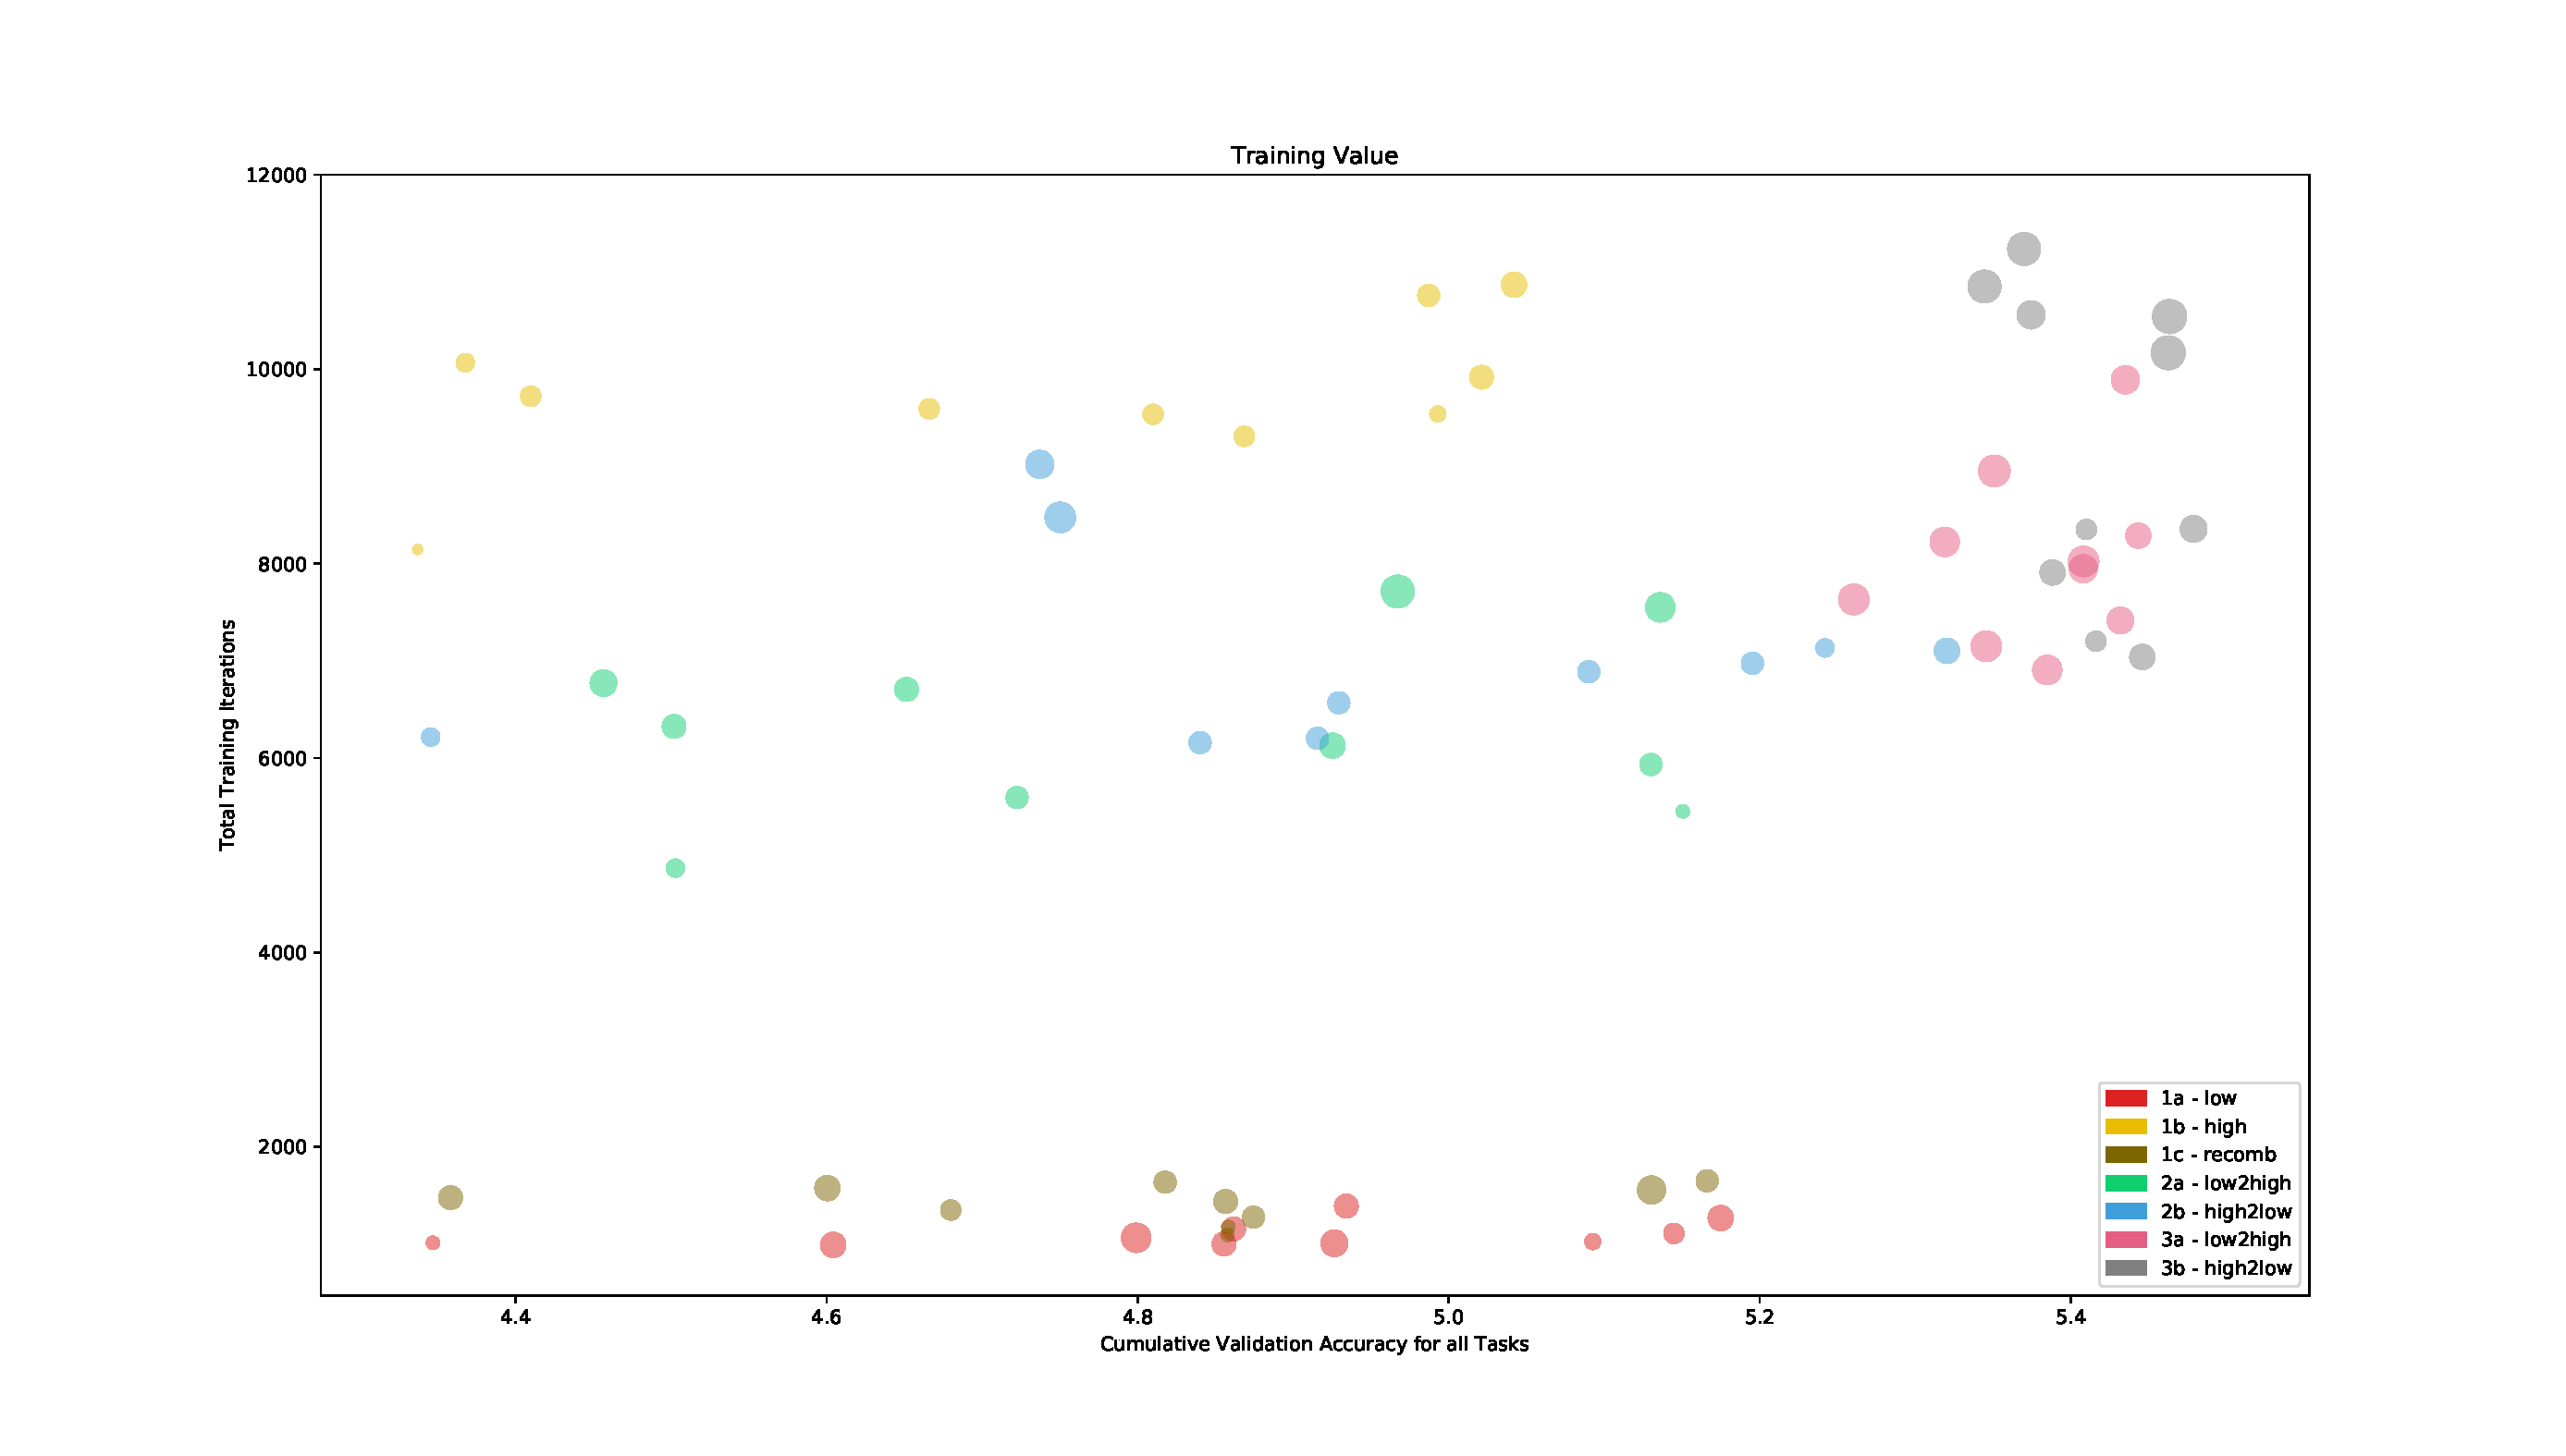
\includegraphics[width=1.2\textwidth,center]{Chapters/Experiments/search_algo/figures/Training_value.pdf}
    \caption{The total amount of training in all optimal paths for each multi-task learning sequence plotted against the cumulative validation accuracy reached for that sequence. The circle size corresponds to the total number of used PathNet modules.}
    \label{fig:search.training_value}
\end{figure}

The training value plot \ref{fig:search.training_value} is the amount of training each multi task sequence went through for all 6 tasks. As expected, algorithms with high tournament size (algorithm 1b) have the higher amount of training units, while the low tournament size algorithms (algorithm 1a and 1c) undergo the least training.

The x axis in this plot is the cumulative validation accuracy for all tasks within the multi task sequences, meaning algorithms that cluster on the right side of the plot have a better accuracy over all. 

Lastly, the circle size reflect how much total capacity was used in the PathNet for each experimental run. Described simply, small circles in the bottom right corner means the algorithm used few weights, took little training and had a good classification accuracy. Comparatively, large circles in the top left corner used a relatively large amount of weights, took long to train and had a low return on investment in classification accuracy. The clear clustering of experimental runs for each algorithm spatially is expected in this plot as the number of training units is easy to predict from the tournament size, however, the clear divide between algorithm 2a and 2b is surprising.

\section{Discussion}
\textit{EDIT NOTE: Rerun of experiments might change results}

Unraveling the amount of information that came as a result of these experimental runs can lean towards the disorienting if not chaotic. In an attempt to be able to discuss the plots mentioned in the previous section, the algorithms are juxtaposed within selection pressure groups first before comparisons are made between them. 

\subsection{Low selection pressure}
Algorithms 1a and 1c have the lowest convergence rate, and as a result of this have also the most gradual changes during each search. Given the modules trained under these algorithms experience the least amount of training we would expect these to reach a lower classification accuracy, but performing a one-way ANOVA test of the null hypothesis
\begin{equation*}
    \label{eq:H0.accuracy.notLowPressure}
    H_{0}:\bar{\mu}_{1_{a}}=\bar{\mu}_{1_{b}}=\bar{\mu}_{1_{c}}=\bar{\mu}_{2_{a}}=\bar{\mu}_{2_{b}}
\end{equation*}
where \(\mu_{x}\) is the mean validation accuracy of algorithm x for some task, gave no p values under the significance level of 0.05\footnote{Significance level 0.05 is used throughout this thesis.}, and the alternate hypothesis
\begin{equation*}
    \label{eq:H0.accuracy.notLowPressure}
    H_{A}:\bar{\mu}_{a_{i}} \neq \bar{\mu}_{a_{j}} 
\end{equation*}
is true for at least one pair of algorithms \(a_{i}\) and \(a_{j}\), where both \(a_{i} \land a_{j} \in A\), and where \(A\) is the set of all algorithms. Looking at figure \ref{fig:search.validation}, the reason for the lowered means for some algorithms in plot \ref{fig:search.accuracy} seems to be caused by an outlier in the data.

\begin{figure}[p!]%[h]
    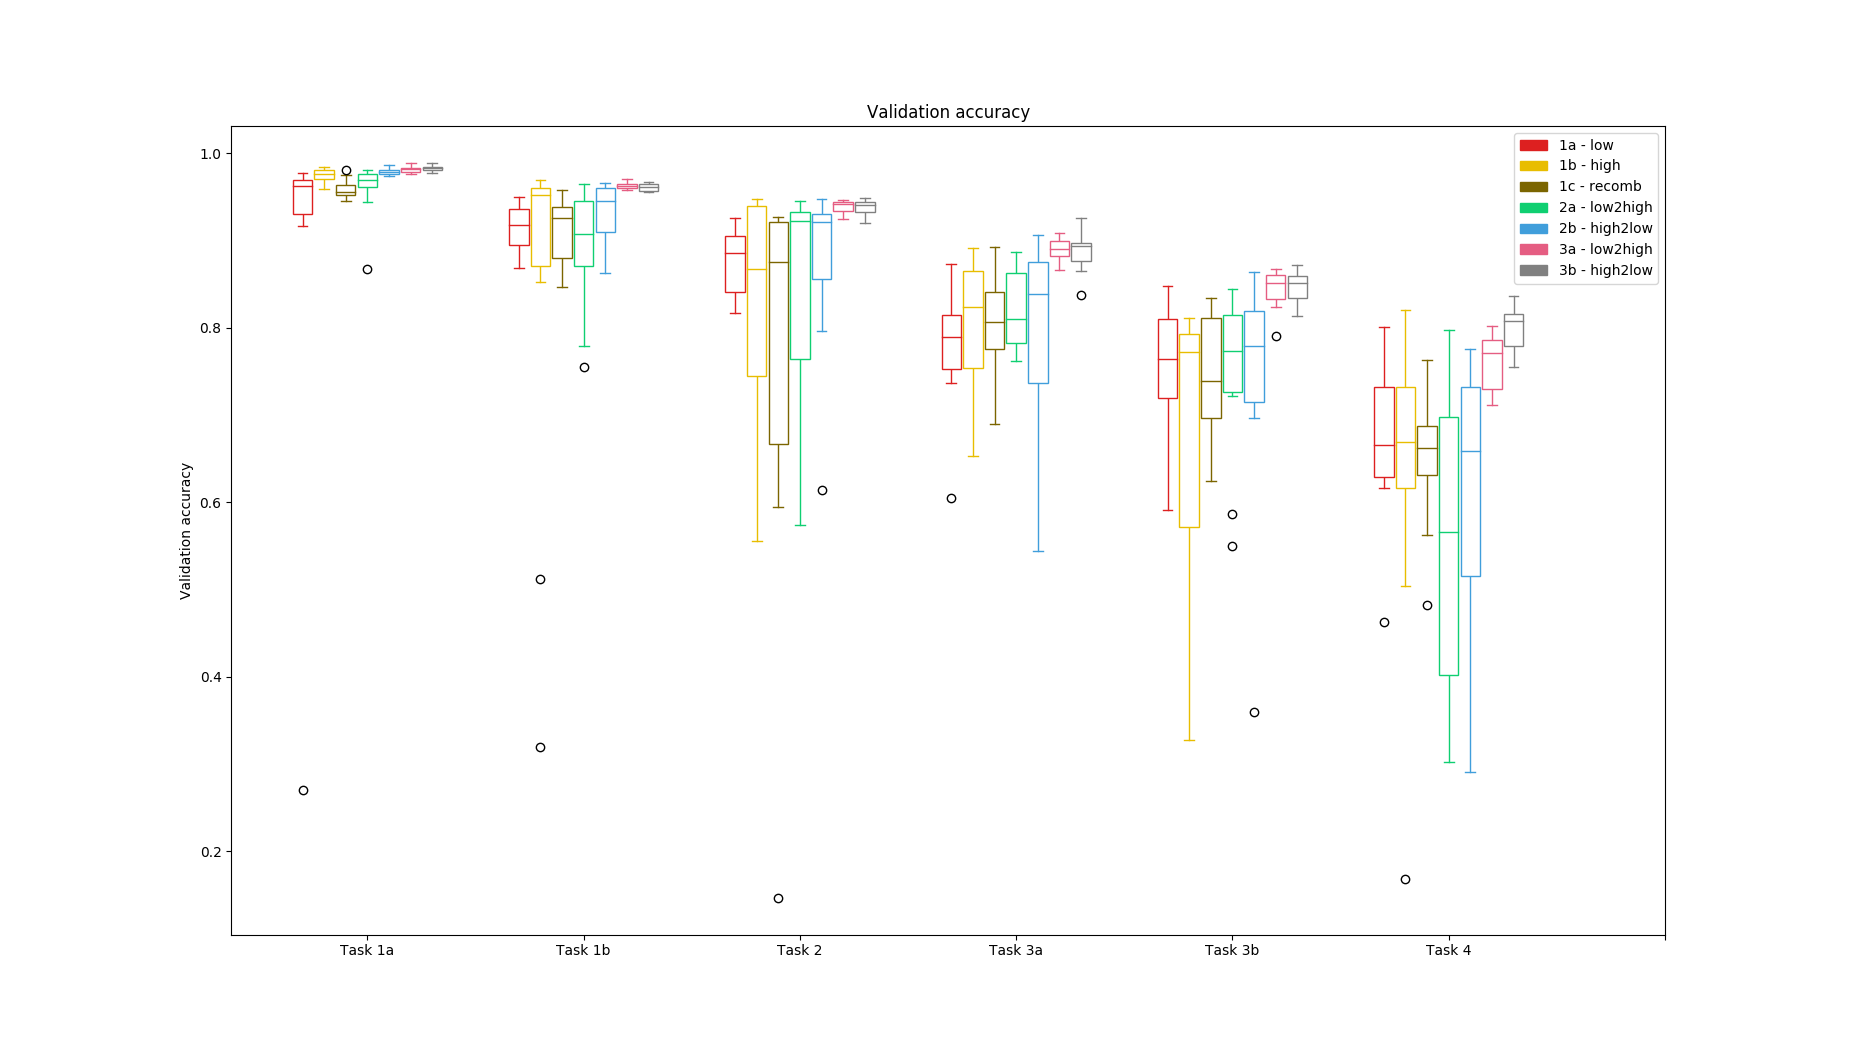
\includegraphics[width=1.2\textwidth, center]{Chapters/Experiments/search_algo/figures/validation_boxplot.png}
    \caption{Boxplot of validation accuracy reached for each task and each algorithm.}
    \label{fig:search.validation}
\end{figure}

Across all metrics, 1a and 1c have about the same performance. An ANOVA test confirm there is no significant difference between the two algorithms validation accuracy means. Plot \ref{fig:search.training_value} shows algorithm 1c trains a bit more on average than 1a, but this is to be expected as the tournament size for algorithm 1c is three while 1a has the lowest size at two, meaning 1c performs 300 evaluations during a search, while 1a performs 200.

During the searches, plot \ref{fig:search.avg_path_size} indicated algorithm 1c tends to yield larger paths on average than 1a, but a significance test of the average size of optimal paths for the two algorithms does not lend confidence to this claim. In fact, no significant difference were found between the average size of selected optimal paths or between the average path size in the final generation in each search, meaning the results shown in \ref{fig:search.avg_path_size} is not significant.

The diversity plots indicates that neither of the algorithms with low selection pressure reaches some state of converged population, where algorithm 1c barely changes. Measuring the diversity of this algorithm as a unique genome frequency does not work, as the recombination makes sure the next generations new genome is not a duplicate unless both parents are equal. The probability of the population having a significant portion being duplicates of each other is to low for this to have a decent chance of happening within the first 100 generations. 

\subsection{Scaling selection pressure}
Algorithms 2a and 2b does not differ in performance from each other or the algorithms with low selection pressure, and they do not have a significant difference for any metric other than module reuse. 

The most prominent feature of plot \ref{fig:search.reuse} is the sudden jump in mean reuse for algorithm 2a in the last task. For task 3b both algorithms kept an average reuse around 5 which makes the jump a value increase of 30\%. While the difference between 2a and algorithms with low or dynamic selection pressure is statistically significant of non-trivial size, it is hard to conclude algorithm 2a leads to the most reuse. Neither of the null-hypotheses \(\bar{\mu}_{2_{a}}=\bar{\mu}_{1_{b}}\) or \(\bar{\mu}_{1_{b}}=\bar{\mu}_{2_{b}}=\bar{\mu}_{1_{a}}=\bar{\mu}_{1_{c}}\) can be rejected, which makes it impossible to say if it is the scaling in tournament sizes that is well suited for reusing modules, or if it is large tournament sizes in general. More experimental runs is needed to conclude either way.  


Regarding convergence rate and diversity metrics, the two algorithms does not produce anything unexpected. Low tournament size leads to low convergence rate and vice versa, meaning both algorithms gradually change between high and low convergence rate depending on whether the algorithm increase or decrease tournament size for each task.

\subsection{Dynamic selection pressure}\label{search-discussion:dynamicselectionpressure}
The last two algorithms 3a and 3b gave the most consistent results for performance and resource demands. They both reach a higher classification accuracy on the validation data which differ significantly from the rest of the algorithms for all tasks on cSVHN. Between them the only performance difference is at the last task where algorithm 3b scores the highest of all algorithms tested with a mean classification accuracy of 80\%\footnote{In the original PathNet paper, a PathNet structure pretrained on the CIFAR set reached a classification accuracy of about 40\% after 500 generations when training on cSVHN with tournament size 2, however the PathNet consisted of fully connected modules and not convolutional operations which is the case here.}.

The trade-off for the comparatively high classification accuracy comes in the amount of training where they train longer than the other algorithms with changing selection pressure (2a and 2b). Using multiple ANOVA tests, mean amount of training units of algorithm 3b does not differ from algorithm 1b, but 1b have a significantly higher training mean than 3a.

Again by using multiple ANOVA tests, the amount of module reuse for algorithms 3a and 3b for task 4 can be shown to not differ from each other but have a lower reuse than all other algorithms. 

\subsection{High selection pressure}
Excluding algorithms 3a and 3b from an ANOVA test tells us there is no significant difference in validation accuracy means for any of the other algorithms, meaning algorithm 1b can not be shown to give better classification accuracy for all its extra training. 
In fact, excluding algorithm 3b which as mentioned undergo the same amount of training, algorithm 1b has a significantly higher mean than every other algorithm and therefore also a much longer run-time. 

In metrics such as reuse and capacity use there is no difference between the algorithms with static selection pressure. 

\section{Conclusion}

The low selection pressure of algorithm 1c causes it to converge towards an optimal path to slowly in this experiment for any benefit from the high exploration rate to become visible. With a lower population size or a higher search termination limit the algorithm might reach a population with such a low diversity so that we could conclude it had found a path from an parametric area of optimal fitness, but at that point the modules would most likely have overfitted to the training data. In a saturated PathNet (see section \ref{section:PNsaturation}) the search problem is reduced from being a optimization of both weights and module selection to just module selection where no overfitting can occur\footnote{Theoretically, overfitting could take place in such a setting. If we imagine the search space is populated with a vast number of optimal modules adapted to contain only small units of memetic knowledge, modules that perform better on training data than validation data could be found. However, this is an unrealistic scenario far from the structure of this PathNet implementation.}, but in that case, another optimization scheme might work better than tournament search. 

To a lesser extent this is true for algorithm 1a also, where it performs similarly to 1c in every metric except for diversity and convergence where the lower tournament size with no recombination has a higher selection pressure and therefore might reach a population state with one optimal path and only duplicates or mutations on that genotype.  

That being said, the performance of these algorithms is no different from those of high selection pressure and therefore high exploitation, so with regards to training time algorithm 1a and 1c is superior to the others where 1a seems to be the better choice for these tasks. 

With no change to accuracy but with 4 to 5 times the training amount over algorithms with low selection pressure, the static high tournament size of algorithm 1b is therefore concluded not to be well suited for this type of search. Algorithms 2a and 2b, while having a lower training amount than 1b, does also not improve on accuracy. 

Best performance is reached with algorithm 3a and 3b, where 3b reaches a higher accuracy for the last task. In plot \ref{fig:search.accuracy}, it looks like 3b is still improving when the search is terminated, hinting at the search termination limit might be to low for this algorithm also. The training amount for these algorithms is around the 9000 iterations mark, meaning the increase in accuracy comes by training significantly more. 



\textit{Edit notes: missing callback to hypothesis and experimental goals}
\chapter{Relearning task}
The motivation behind reusing modules is as mentioned in the introduction, to increase the number of tasks a PathNet can learn before being saturated by decreasing the amount of new capacity a path needs for a new task. A optimal search algorithm for new paths should therefore be able to reuse as much knowledge as possible without limiting the performance. If we assume a ideal search algorithm would find optimal modules for each task, it should be able to find and reuse all learned knowledge if a task is learned twice. 

We can put this to a test by learning some task twice for all seven algorithms in \ref{exp2}. As the amount of module reuse in the first Selection pressure experiment were small, we lower the proverbial bar here by reducing the module search space.

The question we want to answer is this: \textit{"Given optimal conditions for module reuse\footnote{By optimal conditions we mean learning the same task twice in a small PathNet structure.}, which selection pressure scheme is best suited for knowledge reuse?"}

\section{Description}
The experimental structure here is simple. The seven algorithms used in the previous experiments will here be applied to a binary task problem where both tasks are the same: a cSVHN classification problem with all 10 classes. After searching for a optimal path for both tasks, the reuse is noted. 

By performing this experimental trial for each algorithm multiple times, we can compare the observations of reuse with the probability of seeing these results in random path selection, and then with each other. 

\section{Hypothesis}
Based on the reuse in the previous selection pressure experiments, we do not expect any algorithm to yield perfect results \footnote{Perfect results here would constitute finding all modules used in the previous path}, but significantly different from random path selection. Given the algorithms different selection pressures, they are expected to give somewhat different reuse results and I would expect the higher exploration algorithms to yield more reuse, as the amount of parameter optimization needed to give high fitness is small. The advantage the high tournament size algorithms (algorithm 1b and to some degree 2a, 2b, 3a and 3b) have by evaluating more paths should be reduced, as these algorithms have a higher selection pressure and converge quicker. 

\section{Implementation}
The experiment structure here is a binary task problem, where we want to find two paths for a full cSVHN classification problem twice, meaning both task 1 and task 2 is cSVHN classification with all classes. The two searches should have a non-zero probability of reusing no modules, so the PathNet dimensions are set to 3 layers of 6 modules each with a maximum of 3 active modules pr. paths layer. We can describe the total number of possible paths as 
\begin{equation*}
    \prod_{i=0}^{\omega-1}(M-i)^{L}
\end{equation*}
where \(\omega\) is the maximum number of active modules in each layer for each path, \(M\) is the number of modules in each PathNet layer and  \(L\) is the number of layers in the PathNet. This means the number of possible paths in a 20-by-3 PathNet with \(\omega=3\) is  
\begin{equation*}
    \prod_{i=0}^{3-1}(20-i)^{3}\approx 3.2\times10^{11}
\end{equation*}
and in this experiment
\begin{equation*}
    \prod_{i=0}^{3-1}(6-i)^{3}\approx 1.7\times10^{6}
\end{equation*}
Reducing the PathNet size from 20 modules in each layer to 6 have reduced the search space with 5 orders of magnitude, and it should therefore be significantly easier to find reusable modules.

We can approximate the probability of finding any number of reuse by randomly selecting two paths within the limitations of the PathNet dimensions and path-size with a Monte-Carlo approach. Using equation \ref{eq:montecarloP} where we want the probabilities to be minimum 10 times as large as the standard deviation (\(R=0.1\)) and \(n=10^{9}\) Monte-Carlo trials, we calculate the probability accuracy to be 
\begin{equation*}
    \frac{1}{nR^{2}+1}=\frac{1}{10^{7}+1}\approx10^{-7}
\end{equation*}
Meaning we can tell the probability of reuse to the seventh decimal place from the Monte-Carlo results. The results of the performed Monte-Carlo estimation can be found in table \ref{tab:montecarlo}.

\begin{table}[h]
    \centering
    \begin{tabular}{llll}
    \# of reuse & \# of outcomes & Monte-Carlo probabilities & Rounded within uncertainty \\
    0           & 88892859      & 0,088892859               & 0,0888928 \pm 10^{-7}      \\
    1           & 266671854     & 0,266671854               & 0,2666718 \pm 10^{-7}      \\
    2           & 327560805     & 0,327560805               & 0,3275608                  \\
    3           & 213925123     & 0,213925123               & 0,2139251                  \\
    4           & 81393230      & 0,08139323                & 0,0813932                  \\
    5           & 18720470      & 0,01872047                & 0,0187205                  \\
    6           & 2612531       & 0,002612531               & 0,0026125                  \\
    7           & 213747        & 0,000213747               & 0,0002137 \pm 10^{-7}      \\
    8           & 9195          & 0,000009195               & 0,0000092                  \\
    9           & 186           & 0,000000186               & 0,0000002                 
    \end{tabular}
    \caption{Results from Monte-Carlo approximation of reuse probabilities for two paths in a 6-by-3 PathNet with a maximum of 3 active modules in each layer.}
    \label{tab:montecarlo}
\end{table}

For comparison to the experimental results, we will calculate the expected reuse for the number of experimental trial run, and compare the mean reuse value to the mean reuse of each algorithm. The means will be compared through ANOVA tests with a significance level of 0.05  
\section{Results}
\section{Discussion}
\section{Conclusion}

\chapter{Discussion}
Are your results satisfactory? 
Can they be improved? 
Is there a need for improvement? 
Are other approaches worth trying out? 
Will some restriction be lifted? 
Will you save the world with your Nifty Gadget? 

\section{Discussion} 
Discussion of the accuracy and relevance of the results; comparison with other researchers results. 
\subsection{Common errors}
Too far reaching conclusions; guesswork not supported by the data; introduction of a new problem and a discussion around this.  

\section{Conclusion} 
Consequences of the achieved results, for example for new research, theory and applications. 

\subsection{Common errors}
The conclusions are too far reaching with respect to the achieved results; the conclusions do not correspond with the purpose

\newpage
\emergencystretch=2em
\printbibliography
\end{document}

